\Opensolutionfile{ans}[ans/ans-2D4-2]
\section{Biểu diễn hình học của số phức và bài toán liên quan}
\subsection{Kiến thức cơ bản}
\begin{tomtat}
	\begin{enumerate}
		\item Điểm $M(a;b)$ trong hệ trục tọa độ vuông góc của mặt phẳng được gọi là điểm  biểu diễn số phức $z=a+bi$.
		\item Các điểm $M(a;b)$ và  $M'(a;-b)$ biểu diễn số phức $z=a+bi$ và $\overline{z}=a-bi$.
	\end{enumerate}
	\begin{center}
		\begin{tikzpicture}[scale=.7, font=\footnotesize, line join=round, line cap=round, >=stealth]
		\draw[->,line width = 1pt] (-1.5,0)--(-1,0) node[below right]{$O$}--(5,0) node[below]{$x$};
		\draw[->,line width = 1pt] (0,-2.8) --(0,3) node[right]{$y$};
		\foreach \x in {}{
			\draw (\x,0) node[below]{$\x$} circle (1pt);
			\draw (0,\x) node[left]{$\x$} circle (1pt);
		}
		\tkzDefPoints{0/0/O,3/2/M,3/0/H}
		\tkzDrawPoints(O,M)
		\tkzDefPoints{0/0/A,3/2/B}
		\draw[->] (A)--(B);
		\draw (0,2) node[left]{$b$} circle (1pt);
		\draw (3,0) node[below right]{$a$} circle (1pt);
		\draw (3,2) node[above right ]{$M(a; b)$} circle (1pt);
		\draw [dashed] (3,0)--(3,2)--(0,2);
		\draw (0,-2) node[left]{$-b$} circle (1pt);
		\draw (3,-2) node[below right ]{$M'(a; -b)$} circle (1pt);
		\tkzMarkAngles[size=0.7 ,arc=ll](H,O,M)
		\tkzLabelAngles[pos=1,rotate=30](H,O,M){$\varphi$}
		
		
		\draw (7,0) node{$\tan\varphi=\dfrac{b}{a}\cdot$} circle (0pt);
		\draw [dashed] (3,0)--(3,-2)--(0,-2);
		\tkzDefPoints{3/-2/C}
		\draw[->] (A)--(C);
		\end{tikzpicture}
	\end{center}
	\begin{nx}
	Vì điểm biểu diễn của số phức $z=a+bi$ là $M(a;b)$ hay $\overrightarrow{OM}=(a;b)$. Do đó cần nhớ những kiến thức cơ bản về véctơ, hệ trục $Oxy$ và hệ thức lượng trong tam giác.\\
	Cho ham giác $ABC$, hai véctơ $\vec{a}=(a_1;a_2)$, $\vec{b}=(b_1;b_2)$ và $R,\:r,\:p$ lần lượt là bán kính đường tròn ngoại tiếp, nội tiếp và nửa chu vi tam giác $ABC$.
	\begin{enumerate}
		\item Các phép toán cơ bản trên vectơ:
		\begin{itemize}
			\item Quy tắc ba điểm: $\overrightarrow{AB}=\overrightarrow{AC}+\overrightarrow{CA}$, $\overrightarrow{AB}-\overrightarrow{AC}=\overrightarrow{CB}$.
			\item Quy tắc đường chéo hình bình hành $ABCD$: $\overrightarrow{AC}=\overrightarrow{AB}+\overrightarrow{AD}$.
		\end{itemize}
		\item $\overrightarrow{AB}=\left(x_B-x_A;y_B-y_A\right)\Rightarrow AB=\left|\overrightarrow{AB}\right|=\sqrt{\left(x_B-x_A\right)^2+\left(y_B-y_A\right)^2}$.
		\item $M$ là trung điểm của $AB\Rightarrow x_M=\dfrac{x_A+x_B}{2}$ và $y_M=\dfrac{y_A+y_B}{2}$.\\
		$G$ là trọng tâm tam giác $ABC\Rightarrow x_G=\dfrac{x_A+x_B+x_C}{3}$ và $y_G=\dfrac{y_A+y_B+y_C}{3}$.
		\item Hai vectơ bằng nhau: $\vec{a}=\vec{b}\Leftrightarrow\heva{&a_1=b_1\\&a_2=b_2}$.
		\item Hai vectơ cùng phương $\vec{a}\uparrow \uparrow\vec{b}\Leftrightarrow \vec{a}=k.\vec{b}\Leftrightarrow \dfrac{a_1}{b_1}=\dfrac{a_2}{b_2}\:\left(b_1,\:b_2\ne 0\right)$.
		\item Tích vô hướng $\vec{a}.\vec{b}=a_1b_1+a_2b_2=\left|\vec{a}\right|.\left|\vec{b}\right|\cos\left(\vec{a},\vec{b}\right)\Rightarrow\heva{&\vec{a}\bot \vec{b}\Leftrightarrow \vec{a}.\vec{b}=0\\&\cos\left(\vec{a},\vec{b}\right)=\dfrac{\vec{a}.\vec{b}}{\left|\vec{a}\right|.\left|\vec{b}\right|}}$
		\item Định lí hàm sin: $\dfrac{a}{\sin A}=\dfrac{b}{\sin B}=\dfrac{c}{\sin C}=2R$.
		\item
		Định lí hàm cos: $\heva{&a^2=b^2+c^2-2bc.\cos A\\&b^2=a^2+c^2-2ac.\cos B\\&c^2=b^2+a^2-2ab.\cos C}$.
		\begin{center}
			\begin{tikzpicture}[scale=1, font=\footnotesize,line join=round, line cap=round,>=stealth]
			\tkzDefPoints{0/0/B, 1/3/A, 5/0/C}
			\tkzDefMidPoint(B,C)\tkzGetPoint{M}
			\tkzDrawSegments[line width=0.4pt](A,B B,C C,A A,M)
			\tkzDrawPoints(A,B,C,M)
			\tkzLabelSegment[sloped,below,pos=0.6](B,C){$a$}
			\tkzLabelSegment[sloped](C,A){$b$}
			\tkzLabelSegment[sloped](B,A){$c$}
			\tkzLabelSegment[sloped](A,M){$m_a$}
			\tkzLabelPoints[left](A)
			\tkzLabelPoints[below](B,C)
			\end{tikzpicture}
		\end{center}
		\item Công thức trung tuyến: $\heva{&m_a^2=\dfrac{2\left(b^2+c^2\right)-a^2}{4}\\&m_b^2=\dfrac{2\left(a^2+c^2\right)-b^2}{4}\\&m_c^2=\dfrac{2\left(b^2+a^2\right)-c^2}{4}\cdot}$ 
		\item Diện tích: $S=\dfrac{1}{2}ah_a=\dfrac{1}{2}bc\sin A=\dfrac{abc}{4R}=pr=\sqrt{p(p-a)(p-b)(p-c)}$; $p=\dfrac{a+b+c}{2}$: nửa chu vi.
	\end{enumerate}
\end{nx}
	\underline{\textbf{Bài toán:}} Trong mặt phẳng tọa độ $Oxy$, hãy tìm tập hợp các điểm $M(x;y)$ biểu diễn số phức $z=x+yi$ thỏa mãn điều kiện cho trước.
	\begin{itemize}
		\item Bước 1: Gọi $M(x;y)$ biểu diễn số phức $z=x+yi$ (với $x, y\in\mathbb{R}$)
		\item Bước 2 : Biến đổi điều kiện $K$ để tìm mối liên hệ giữa $x$, $y$  và kết luận.
	\end{itemize}
	\begin{center}
		\begin{tabular}{|l|p{7.5cm}|}
			\hline 
			\textbf{Mối liên hệ giữa $x$ và $y$}& \textbf{Kết luận tập hợp điểm $M(x;y)$ }\\ 
			\hline 
			$\circ Ax+By+C=0$ & Là đường thẳng $d\colon Ax+By+C=0$.\\ 
			\hline 
			$\circ (x-a)^2+(y-b)^2=R^2$ & Là đường tròn $(C)$ có tâm $I(a;b)$ và bán kính $R$.\\ 
			\hline 
			$\circ x^2+y^2+2ax+2by+c=0$ & Là đường tròn $(C)$ có tâm $I(-a;-b)$ và bán kính $R=\sqrt{a^2+b^2-c}$.\\ 
			\hline 
			$\circ (x-a)^2+(y-b)^2\leq R^2$ & Là hình tròn $(C)$ có tâm $I(a;b)$ và bán kính $R$.\\ 
			\hline 
			$\circ x^2+y^2+2ax+2by+c\leq 0$ & Là hình tròn $(C)$ có tâm $I(-a;-b)$ và bán kính $R=\sqrt{a^2+b^2-c}$.\\ 
			\hline 
			$\circ R_1^2\leq (x-a)^2+(y-b)^2\leq R_2^2$ & Là hình vành khăn tạo bởi hai đường tròn đồng tâm $I(a;b)$ và bán kính $R_1$ và $R_2$.\\ 
			\hline 
			$\circ y=ax^2+bx+c$ & Là Parabol $(P)$ có đỉnh $I\left( -\dfrac{b}{2a};-\dfrac{\Delta}{4a}\right) $.\\ 
			\hline 
			$\circ \dfrac{x^2}{a^2}+\dfrac{y^2}{b^2}=1$ với 
			$\heva{MF_1+MF_2=2a &\\ F_1F_2=2c<2a& }$ & Là đường Elip $(E)$ có trục lớn  $2a$, trục nhỏ $2b$ và tiêu cự $2c=2\sqrt{a^2-b^2}$.\\ 
			\hline 
			$\circ \left| \overrightarrow{MA}\right|= \left| \overrightarrow{MB}\right|$ & Là đường trung trực của đoạn $AB$.\\ 
			\hline 
		\end{tabular} 
	\end{center}
\end{tomtat}
\subsection{Bài tập vận dụng}
\begin{dang}{Bài toán xác định điểm biểu diễn số phức cơ bản và bài toán liên quan}
\end{dang}
%\begin{listEX}
\begin{ex}%[Ngô Quang Anh, 12-EX-1-DCHT]%[2D4Y1-2] 
	Quan sát hình vẽ bên cạnh, ta có:
	\immini{	Điểm $A(2;1)$ biểu diễn cho số phức $z_1=2+i$.\\
		Điểm $B(\ldots;\ldots)$ biểu diễn cho số phức $z_2=\ldots$.\\
		Điểm $C(\ldots;\ldots)$ biểu diễn cho số phức $z_3=\ldots$.\\
		Điểm $D(\ldots;\ldots)$ biểu diễn cho số phức $z_4=\ldots$.\\
		Điểm $E(\ldots;\ldots)$ biểu diễn cho số phức $z_5=\ldots$.\\
		Điểm $F(\ldots;\ldots)$ biểu diễn cho số phức $z_6=\ldots$.}
	{	\begin{tikzpicture}[>=stealth, scale= 1,samples=1000,smooth,color=black,line width=0.6pt,xscale=1,yscale=1]
		\draw[->] (-3.5,0) -- (3.5,0) node[below] { $x$};
		\draw[->] (0,-2.5) -- (0,3.5) node[below right] {$y$};
		\draw (0,0) node[below right] {\footnotesize $O$};
		\draw[dashed] (2,0)--(2,1)--(0,1) (2,0)--(2,-1)--(0,-1);
		\fill (2,1) circle (1.5pt);  
		\fill (2,-1) circle (1.5pt);  
		\draw (2,1) node[right]{$A$} (2,-1) node[right]{$B$};
		\draw[dashed] (1,0)--(1,3)--(0,3) (0,0)--(0,2)--(0,2);
		\fill (1,3) circle (1.5pt);  
		\fill (0,2) circle (1.5pt);  
		\draw (1,3) node[above]{$C$} (0,2) node[above right]{$D$};
		\draw[dashed] (-3,0)--(-3,2)--(0,2) (-1,0)--(-1,-2)--(0,-2);
		\fill (-3,2) circle (1.5pt);  
		\fill (-1,-2) circle (1.5pt);  
		\draw (-3,2) node[left]{$E$} (-1,-2) node[left]{$F$};
		\foreach \x in {-3,-1,1,2}
		\draw[thin] (\x,1pt)--(\x,-1pt) node [below left] {$\x$};
		\foreach \y in {-2,-1,1,2,3}
		\draw[thin] (1pt,\y)--(-1pt,\y) node [above left] {$\y$};
		\end{tikzpicture}}
	\dapso{$B(2; -1), z_2=2-i$; $C(1; 3), z_3=1+3i$; $D(0; 2), z_4=2i$; $E(-3; 2), z_5=-3+2i$; $F(-1;-2), z_2=-1-2i$.}
\end{ex}
\begin{note}
	Số phức $z_1=2+i$ và số phức liên hợp $\overline {z}_1=z_2=2-i$ có điểm biểu diễn trên mặt phẳng tọa độ $Oxy$ là $A$ và $B$ đối xứng nhau qua trục $Ox$.
\end{note}
\begin{ex}%[Ngô Quang Anh, 12-EX-1-DCHT]%[2D4Y1-1]
	Điểm $A$ trong hình vẽ dưới đây là điểm biểu diễn của số phức $z$.
	\immini{Tìm phần thực và phần ảo của số phức $\overline{z}$.
		\choice
		{Phần thực là $-3$ và phần ảo là $2i$}
		{\True Phần thực là $3$ và phần ảo là $-2$}
		{Phần thực là $3$ và phần ảo là $-2i$}
		{Phần thực là $-3$ và phần ảo là $-2$}}
	{\begin{tikzpicture}[>=stealth, scale= 1,samples=1000,smooth,color=black,line width=0.6pt,xscale=1,yscale=1]
		\draw[->] (-0.5,0) -- (3.5,0) node[below] { $x$};
		\draw[->] (0,-0.5) -- (0,2.5) node[below right] {$y$};
		\draw (0,0) node[below right] {\footnotesize $O$};
		\foreach \x in {3}
		\draw[thin] (\x,1pt)--(\x,-1pt) node [below] {$\x$};
		\foreach \y in {2}
		\draw[thin] (1pt,\y)--(-1pt,\y) node [left] {$\y$};
		\draw[dashed] (3,0)--(3,2)--(0,2);
		\fill (3,2) circle (1.5pt);    
		\draw (3,2) node[above]{$A$};
		\end{tikzpicture}}
	
	\loigiai{
		Số phức $z=3+2i$ nên  số phức liên hợp $\overline {z}=3-2i$.\\
		Vậy $\overline{z} $ có phần thực là $3$ và phần ảo là $-2$.
	}
\end{ex}
\begin{ex}%[Ngô Quang Anh, 12-EX-1-DCHT]%[2D4Y2-2]
	Cho số phức $z=2-i$. Trên mặt phẳng tọa độ, tìm điểm biểu diễn số phức $w=iz$.
	\choice
	{$M(-1;2)$}
	{$N(2;-1)$}
	{$P(2;1)$}
	{\True $Q(1;2)$}
	\loigiai{
		$w=iz=i(2-i)=2i-i^2=1+2i$. Suy ra điểm biểu diễn số phức $w=iz$ là $Q(1;2)$. 
	}
\end{ex}
\begin{ex}%[Ngô Quang Anh, 12-EX-1-DCHT]%[2D4B3-2] 
	Cho số phức $z$ thỏa mãn $2i+z(1-i)=i(3-i)$. Trên mặt phẳng tọa độ $Oxy$, điểm nào dưới đây là điểm biểu diễn số phức $z$.
	\choice
	{$M_3(1;0)$}
	{\True $M_1(0;1)$}
	{$M_4(0;2)$}
	{$M_2(0;-1)$}
	\loigiai{
		Ta có: $2i+z(1-i)=i(3-i)\Leftrightarrow z=\dfrac{i(3-i)-2i}{1-i}=\dfrac{1+i}{1-i}=i$.\\
		Suy ra điểm biểu diễn số phức $z$ là $M_1(0;1)$.
	}
\end{ex}
\begin{ex}%[Ngô Quang Anh, 12-EX-1-DCHT]%[2D4B2-2]
	Cho số phức $z=3-2i$. Tìm điểm biểu diễn của số phức $w=z+i\cdot \overline{z}$.
	\choice
	{$A(1;-5)$}
	{ $M(5;-5)$}
	{\True $M(1;1)$}
	{$M(5;1)$}
	\loigiai{
		Ta có: $w=z+i\cdot \overline{z}=3-2i+i\cdot (3+2i)=3-2i+3i+2i^2=3-2i+3i-2=1+i$.\\
		Suy ra điểm biểu diễn số phức $w$ là $M(1;1)$.
	}
\end{ex}
\begin{ex}%[Ngô Quang Anh, 12-EX-1-DCHT]%[2D4B2-3] 
	Điểm $M(x_0;y_0)$ biểu diễn của số phức $z$ thỏa $(1+i)z+(2+i)\overline{z}=3+i$. Tính $2x_0+3y_0$.
	\choice
	{$-1$}
	{$8$}
	{\True $5$}
	{$1$}
	\loigiai{ 
		Do $M(x_0;y_0)$ biểu diễn của số phức $z$ nên $z=x_0+y_0i$.\\
		Ta có: \\
		$(1+i)(x_0+y_0i)+(2+i)(x_0-y_0i)=3+i
		\Leftrightarrow 3x_0+(2x_0-y_0)i=3+i\Leftrightarrow \heva{&3x_0=3\\&2x_0-y_0=1}\Leftrightarrow \heva{&x_0=1\\&y_0=1.}
		$\\
		Vậy $2x_0+3y_0=2+3=5$.
	}
\end{ex}

\begin{ex}%[Ngô Quang Anh, 12-EX-1-DCHT]%[2D4B1-1]
	Cho hai số phức $z_1=1-3i$,  $z_2=-4-6i$ có các điểm biểu diễn trong mặt phẳng tọa độ lần lượt là $M$, $N$. Gọi $z$ là số phức mà có  điểm biểu diễn là trung điểm đoạn $MN$. Tính mô-đun của số phức $z$.
	\choice
	{$\left|z \right|=3\sqrt{10}$}
	{ $\left|z \right|=\dfrac{2\sqrt{10}}{3}$}
	{$\left|z \right|=\sqrt{10}$}
	{\True $\left|z \right|=\dfrac{3\sqrt{10}}{2} $}
	\loigiai{
		Ta có $ M(1;-3)$ và $N(-4;-6)$.\\
		$I$ là trung điểm đoạn $MN$ nên $I\left(-\dfrac{3}{2};-\dfrac{9}{2}\right) $.\\
		Mà $z$ là số phức có  điểm biểu diễn là trung điểm $I$ đoạn $MN$ nên $z=-\dfrac{3}{2}-\dfrac{9}{2}i$.\\
		Vậy $\left|z \right|=\dfrac{3\sqrt{10}}{2} $.		
	}
\end{ex}


\begin{ex}%[Ngô Quang Anh, 12-EX-1-DCHT]%[2D4B2-2]
	Gọi $M$ và $N$ lần lượt là điểm biểu diễn của các số phức $z_1,\:z_2$ như hình bên dưới.
	\immini{Hỏi khẳng định nào sau đây {\bf sai}?
		\haicot
		{$\left|z_1-z_2\right|=MN$}
		{$\left|z_1\right|=OM$}
		{$\left|z_2\right|=ON$}
		{\True $\left|z_1+z_2\right|=MN$}
	}
	{
		\begin{tikzpicture}[>=stealth, scale= 1,samples=1000,smooth,color=black,line width=0.6pt,xscale=1,yscale=1]
		\draw[->] (-2.5,0) -- (1,0) node[below] { $x$};
		\draw[->] (0,-0.5) -- (0,2.5) node[below right] {$y$};
		\draw (0,0) node[below right] {\footnotesize $O$};
		\draw[dashed] (-1,0)--(-1,2)--(0,2) (-2,0)--(-2,1)--(0,1);
		\fill (-1,2) circle (1.5pt);  
		\fill (-2,1) circle (1.5pt);  
		\draw (-1,2) node[above]{$N$} (-2,1) node[above]{$M$};
		\end{tikzpicture}
	}
	\loigiai{
		Đặt $z_1=a_1+b_1i,\:z_2=a_2+b_2i$, suy ra $M(a_1;b_1),\:N(a_2;b_2)$\\
		$\Rightarrow MN=\sqrt{\left(a_2-a_1\right)^2+\left(b_2-b_1\right)^2}$.\\
		Ta có $z_1+z_2=\left(a_1+a_2\right)+\left(b_1+b_2\right)i\Rightarrow \left|z_1+z_2\right|=\sqrt{\left(a_1+a_2\right)^2+\left(b_1+b_2\right)^2}\ne MN$.
	}
\end{ex}
%%%
\begin{ex}%[Ngô Quang Anh, 12-EX-1-DCHT]%[2D4B2-2]
	Gọi $M$ là điểm biểu diễn số phức $z_1=3-4i$ và điểm $N$ là điểm biểu diễn số phức $z_2=\dfrac{1}{2}\left(1+i\right)z_1$. Tính diện tích $S$ của tam giác $OMN$ với $O$ là gốc tọa độ.
	\choice
	{$S=\dfrac{15}{2}$}
	{\True $S=\dfrac{25}{4}$}
	{$S=\dfrac{25}{2}$}
	{$S=\dfrac{31}{4}$}
	\loigiai{
		Ta có $z_1=3-4i$, $z_2=\dfrac{1}{2}\left(1+i\right)z_1=\dfrac{7}{2}-\dfrac{1}{2}i\Rightarrow M(3;-4),\:N\left(\dfrac{7}{2};-\dfrac{1}{2}\right)$.\\
		Ta có $\overrightarrow{NO}=\left(-\dfrac{7}{2};\dfrac{1}{2}\right),\:\overrightarrow{NM}=\left(-\dfrac{1}{2};-\dfrac{7}{2}\right)\Rightarrow \overrightarrow{NO}.\overrightarrow{NM}=0\Rightarrow \triangle OMN$ vuông tại $N$.\\
		$NO=\dfrac{5\sqrt{2}}{2}$ và $NM=\dfrac{5\sqrt{2}}{2}$.\\
		Vậy $S_{\triangle OMN}=\dfrac{1}{2}\cdot NO\cdot NM=\dfrac{25}{4}$.
	}
\end{ex}
\textbf{Cần nhớ: }{\it Tính diện tích $\triangle ABC:\heva{&\overrightarrow{AB}=(a;b)\\&\overrightarrow{AC}=(c;d)}\Rightarrow S_{\triangle ABC}=\dfrac{1}{2}\begin{vmatrix}
	a&b\\ 
	c&d\\ 
	\end{vmatrix}=\dfrac{1}{2}\left|ad-bc\right|$}.
\begin{ex}%[Ngô Quang Anh, 12-EX-1-DCHT]%[2D4B2-2]
	Trong mặt phẳng phức cho $3$ điểm lần lượt là điểm biểu diễn của số phức $z_1=1+i,\:z_2=\left(1+i\right)^2,\:z_3=m-i$. Tìm tham số $m$ để tam giác $ABC$ vuông tại $B$.
	\choice
	{$m=3$}
	{$m=-2$}
	{\True $m=-3$}
	{$m=2$}
	\loigiai{
		Ta có $z_1=1+i\Rightarrow A(1;1)$, $z_1=(1+i)^2=2i\Rightarrow B(0;2)$, $z_3=m-i\Rightarrow C(m,-1)$.\\
		$\overrightarrow{BA}=(1;-1)$, $\overrightarrow{BC}=(m;-3)$.\\
		Để $\triangle ABC$ vuông tại $B\Leftrightarrow \overrightarrow{BA}.\overrightarrow{BC}=0\Leftrightarrow 1\cdot m+(-1)\cdot (-3)=0\Leftrightarrow m+3=0\Leftrightarrow m=-3$.
	}
\end{ex}
\begin{ex}%[Ngô Quang Anh, 12-EX-1-DCHT]%[2D4B1-2]
	Trong mặt phẳng phức, gọi $A,\:B,\:C$ lần lượt là điểm biểu diễn của các số phức $z_1=3+2i,\:z_2=3-2i,\:z_3=-3-2i$. Hỏi khẳng định nào sau đây là {\bf sai}?
	\choice
	{$B$ và $C$ đối xứng nhau qua trục tung}
	{\True Trọng tâm của tam giác $ABC$ là điểm $G\left(1;\dfrac{2}{3}\right)$}
	{$A$ và $B$ đối xứng nhau qua trục hoành}
	{$A,\:B,\:C$ nằm trên đường tròn tâm là gốc tọa độ và bán kính bằng $\sqrt{13}$}
	\loigiai{
		Ta có $z_1=3+2i\Rightarrow A(3;2),\:z_2=3-2i\Rightarrow B(3;-2),\:z_3=-3-2i\Rightarrow C(-3;-2)$.\\
		$B$ và $C$ đối xứng nhau qua trục tung.\\
		Trọng tâm $G$ của tam giác $ABC$: $G\left(1;-\dfrac{2}{3}\right)\ne \left(1;\dfrac{2}{3}\right)$.\\
		$A$ và $B$ đối xứng nhau qua trục hoành.\\
		$OA=OB=OC=\sqrt{13}$ nên  $A,\:B,\:C$ nằm trên đường tròn tâm là gốc tọa độ và bán kính bằng $\sqrt{13}$.
	}
\end{ex}

\begin{ex}%[Ngô Quang Anh, 12-EX-1-DCHT]%[2D4B1-2]
	Cho $ABCD$ là hình bình hành với $A, B, C$ lần lượt là các điểm biểu diễn các số phức $1-i,~2+3i,~3+i$. Tìm số phức $z$ có điểm biểu diễn là $D$.
	\choice
	{\True $z=2-3i$}
	{$z=4+5i$}
	{$z=4+3i$}
	{$z=2+5i$}
	\loigiai{Ta có $A(1;-1), B(2;3), C(3;1)$.\\Gọi $z=x+yi~ (x,y\in\mathbb{R})\Rightarrow D(x;y)$. Khi đó $\overrightarrow{AB}=\left(1;4\right), \overrightarrow{DC}=\left(3-x; 1-y\right)$.\\
		Do $ABCD$ là hình bình hành nên $\overrightarrow{AB}=\overrightarrow{DC}\Leftrightarrow\heva{&1=3-x\\&4=1-y}\Leftrightarrow\heva{&x=2\\&y=-3.}$\\ Vậy $z=2-3i$.
	}
\end{ex}
\begin{ex}%[Ngô Quang Anh, 12-EX-1-DCHT]%[2D4B1-2]
	\immini
	{
		Cho hai điểm $M, N$ trong mặt phẳng phức như hình vẽ, gọi $P$ là điếm sao cho $OMNP$ là hình bình hành. Hỏi điểm $P$ biểu thị cho số phức nào sau đây?
		\choice
		{$z_4=3-3i$} 
		{$z_3=-2+i$}
		{$z_2=4+i$}
		{\True $z_1=2-i$}
	}
	{
		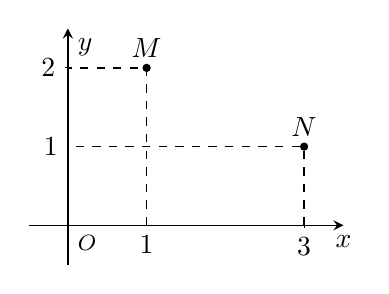
\begin{tikzpicture}[>=stealth, scale= 1,samples=1000,smooth,color=black,line width=0.6pt,xscale=1,yscale=1]
		\draw[->] (-0.5,0) -- (3.5,0) node[below] { $x$};
		\draw[->] (0,-0.5) -- (0,2.5) node[below right] {$y$};
		\draw (0,0) node[below right] {\footnotesize $O$};
		\foreach \x in {3}
		\draw[thin] (\x,1pt)--(\x,-1pt) node [below] {$\x$};
		\foreach \y in {2}
		\draw[thin] (1pt,\y)--(-1pt,\y) node [left] {$\y$};
		\draw[dashed] (1,0)--(1,2)--(0,2);
		\draw[dashed] (3,0)--(3,1)--(0,1);
		\fill (3,1) circle (1.5pt); 
		\fill (1,2) circle (1.5pt);     
		\draw (3,1) node[above]{$N$};
		\draw (1,2) node[above]{$M$};
		\draw (0,1) node[left]{$1$} circle (0pt);
		\draw (1,0) node[below]{$1$} circle (0pt);
		\end{tikzpicture}
	}
	\loigiai{
		Ta có $O(0; 0), M(1;2), N(3;1)$ và $OMNP$ là hình bình hành $\Rightarrow P(2;-1)$ $\Rightarrow P$ biểu thị số phức $z_1=2-i$.
	}
\end{ex}
\begin{ex}%[Ngô Quang Anh, 12-EX-1-DCHT]%[2D4B1-2]
	Trong mặt phẳng phức, gọi $A, B, C$ lần lượt là các điểm biểu diễn các số phức $z_1=\left(1-i\right)\cdot\left(2+i\right), z_2=1+3i, z_3=-1-3i$. Hỏi khẳng định nào sau đây đúng?
	\choice
	{Tam giác $ABC$ là tam giác vuông nhưng không cân}
	{Tam giác $ABC$ là tam giác cân nhưng không đều, không vuông}
	{\True Tam giác $ABC$ là tam giác vuông cân}
	{Tam giác $ABC$ là tam giác đều}
	\loigiai{Ta có $z_1=3-i$ nên $A\left(3;-1\right), B\left(1; 3\right), C\left(-1;-3\right)$. Khi đó $\overrightarrow{AB}=\left(-2;4\right), \overrightarrow{AC}=\left(-4;-2\right), \overrightarrow{BC}=\left(-2;-6\right)$.\\Do $\heva{&\overrightarrow{AB}\cdot\overrightarrow{AC}=0\\&AB=AC=2\sqrt{5}}$ nên tam giác $ABC$ vuông cân tại $A$.}
\end{ex}

\begin{ex}%[Ngô Quang Anh, 12-EX-1-DCHT]%[2D4B1-2]
	\immini
	{Cho số phức $z$ thỏa $\left|z\right|=2\sqrt{10}$. Hỏi điểm biểu diễn của $z$ là điểm nào trong hình?
		\choice
		{Điểm $P$}
		{Điểm $M$}
		{Điểm $N$}
		{\True Điểm $Q$}
	}
	{
		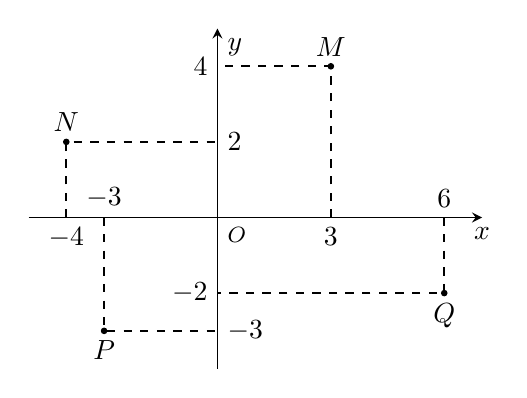
\begin{tikzpicture}[>=stealth, scale= 0.8,color=black,line width=0.6pt,xscale=0.6,yscale=0.6]
		\draw[->] (-5,0) -- (7,0) node[below] { $x$};
		\draw[->] (0,-4) -- (0,5) node[below right] {$y$};
		\draw (0,0) node[below right] {\footnotesize $O$};
		\draw[dashed] (3,0)--(3,4)--(0,4);
		\draw[dashed] (6,0)--(6,-2)--(0,-2);
		\draw[dashed] (-3,0)--(-3,-3)--(0,-3);
		\draw[dashed] (-4,0)--(-4,2)--(0,2);
		\fill (6,-2) circle (2.5pt); 
		\fill (3,4) circle (2.5pt);
		\fill (-4,2) circle (2.5pt); 
		\fill (-3,-3) circle (2.5pt);     
		\draw (3,4) node[above]{$M$};
		\draw (6,-2) node[below]{$Q$};
		\draw (-4,2) node[above]{$N$};
		\draw (-3,-3) node[below]{$P$};
		\draw (0,-2) node[left]{$-2$} circle (0pt);
		\draw (0,4) node[left]{$4$} circle (0pt);
		\draw (-4,0) node[below]{$-4$} circle (0pt);
		\draw (3,0) node[below]{$3$} circle (0pt);
		\draw (0,-3) node[right]{$-3$} circle (0pt);
		\draw (0,2) node[right]{$2$} circle (0pt);
		\draw (-3,0) node[above]{$-3$} circle (0pt);
		\draw (6,0) node[above]{$6$} circle (0pt);
		\end{tikzpicture}
	}	
	\loigiai{Ta có: $M\left(3;4\right)\Rightarrow\left|z\right|=5$, $N\left(-4;2\right)\Rightarrow\left|z\right|=2\sqrt{5}$, $P\left(-3;-3\right)\Rightarrow\left|z\right|=3\sqrt{2}$, $Q\left(6;-2\right)\Rightarrow\left|z\right|=2\sqrt{10}$.}
\end{ex}

\begin{ex}%[Ngô Quang Anh, 12-EX-1-DCHT]%[2D4B1-2]
	\immini
	{
		Trong mặt phẳng tọa độ, điểm $M$ là điểm biểu diễn số phức $z$. Điểm nào trong hình vẽ là điểm biểu diễn của số phức $2z$?
		\choice
		{Điểm $N$}
		{Điểm $Q$}
		{\True Điểm $E$}
		{Điểm $P$}
	}
	{
		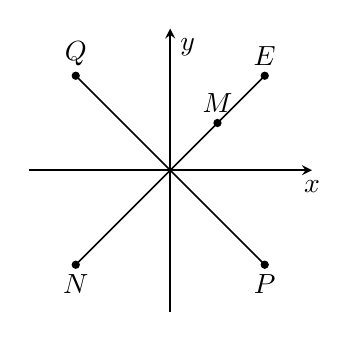
\begin{tikzpicture}[>=stealth, scale= 1,color=black,line width=0.6pt,xscale=0.6,yscale=0.6]	
		\draw[->] (-3,0) -- (3,0) node[below] { $x$};
		\draw[->] (0,-3) -- (0,3) node[below right] {$y$};
		\fill (1,1) circle (2.5pt); 
		\fill (2,2) circle (2.5pt);
		\fill (2,-2) circle (2.5pt); 
		\fill (-2,-2) circle (2.5pt);
		\fill (-2,2) circle (2.5pt);     
		\draw (1,1) node[above]{$M$};
		\draw (2,2) node[above]{$E$};
		\draw (2,-2) node[below]{$P$};
		\draw (-2,2) node[above]{$Q$};
		\draw (-2,-2) node[below]{$N$};
		\draw (-2,-2)--(2,2);
		\draw (-2,2)--(2,-2);		
		\end{tikzpicture}
	}
	\loigiai{Dựa vào hình vẽ ta thấy $\overrightarrow{OE}=2\overrightarrow{OM}$.\\ Vậy điểm $E$ là điểm biểu diễn của số phức $2z$.}
\end{ex}

\begin{ex}%[Ngô Quang Anh, 12-EX-1-DCHT]%[2D4B3-2]
	\immini
	{
		Cho số phức $z$ có điểm biểu diễn là $M$. Biết số phức $w=\dfrac{1}{z}$ được biểu diễn bởi một trong bốn điểm $P, Q, R, S$ như hình vẽ. Hỏi điểm biểu diễn của $w$ là điểm nào?
		\choice
		{Điểm $S$}
		{\True Điểm $Q$}
		{Điểm $P$}
		{Điểm $R$}
	}
	{
		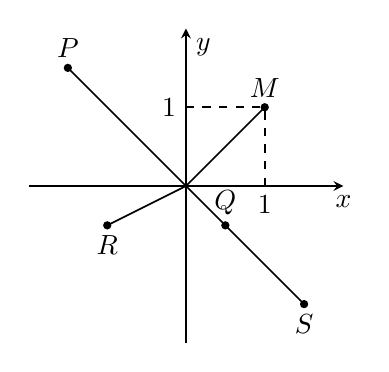
\begin{tikzpicture}[>=stealth, scale= 1,color=black,line width=0.6pt,xscale=1,yscale=1]	
		\draw[->] (-2,0) -- (2,0) node[below] { $x$};
		\draw[->] (0,-2) -- (0,2) node[below right] {$y$};
		\fill (1,1) circle (1.5pt); 
		\fill (0.5,-0.5)  circle (1.5pt);
		\fill (1.5,-1.5) circle (1.5pt); 
		\fill (-1.5,1.5) circle (1.5pt);
		\fill (-1,-0.5) circle (1.5pt);     
		\draw (1,1) node[above]{$M$};
		\draw (0.5,-0.5) node[above]{$Q$};
		\draw (1.5,-1.5) node[below]{$S$};
		\draw (-1.5,1.5) node[above]{$P$};
		\draw (-1,-0.5) node[below]{$R$};
		\draw (-1.5,1.5)--(1.5,-1.5);
		\draw (0,0)--(-1,-0.5);	
		\draw (0,0)--(1,1);	
		\draw[dashed] (1,0)--(1,1)--(0,1);
		\draw (0,1) node[left] {$1$};
		\draw (1,0) node[below] {$1$};	
		\end{tikzpicture}
	}
	
	\loigiai{Ta có $M\left(1;1\right)$ nên $z=1+i$, suy ra $w=\dfrac{1}{z}=\dfrac{1}{1+i}=\dfrac{1}{2}-\dfrac{1}{2}i$.\\Vậy điểm biểu diễn của $w$ là điểm $Q$.}
\end{ex}

\begin{ex}%[Ngô Quang Anh, 12-EX-1-DCHT]%[2D4B3-2]
	\immini
	{
		Số phức $z$ được biểu diễn trên mặt phẳng tọa độ như hình vẽ. Hỏi điểm biểu diễn của số phức $w=\dfrac{i}{\overline{z}}$ nằm ở góc phần tư thứ mấy trong hệ trục tọa độ $Oxy$?
		\choice
		{Thứ nhất}
		{\True Thứ hai}
		{Thứ ba}
		{Thứ tư}
	}
	{
		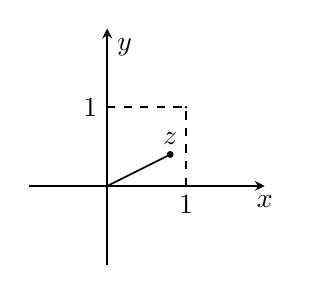
\begin{tikzpicture}[>=stealth, scale= 1,color=black,line width=0.6pt,xscale=1,yscale=1]	
		\draw[->] (-1,0) -- (2,0) node[below] { $x$};
		\draw[->] (0,-1) -- (0,2) node[below right] {$y$};
		\fill (1,1) circle (0.5pt);
		\fill (0.8,0.4) circle (1.25pt);       
		\draw (0.8,0.4) node[above]{$z$};
		\draw (0,0)--(0.8,0.4);	
		\draw[dashed] (1,0)--(1,1)--(0,1);
		\draw (0,1) node[left] {$1$};
		\draw (1,0) node[below] {$1$};	
		\end{tikzpicture}
	}
	
	\loigiai{
		Gọi $z=x+yi$, $(x, y\in\mathbb{R^+})$ sao cho $0<x^2+y^2<\sqrt{2}$. Khi đó\\
		$$w=\dfrac{i}{\overline{z}}=\dfrac{i}{x-yi}=\dfrac{i(x+yi)}{x^2+y^2}=\dfrac{-y+xi}{x^2+y^2}=-\dfrac{y}{x^2+y^2}+\dfrac{x}{x^2+y^2}i.$$ Mà $-\dfrac{y}{x^2+y^2}<0; \dfrac{x}{x^2+y^2}>0$ $\Rightarrow$ điểm biểu diễn của số phức $w$ nằm ở góc phần tư thứ hai.
	}
\end{ex}	

\begin{ex}%[Ngô Quang Anh, 12-EX-1-DCHT]%[2D4K3-2]
	\immini
	{
		Cho số phức $z$ thỏa $\left|z\right|=\dfrac{\sqrt{2}}{2}$ và điểm $A$ trong hình vẽ bên là điểm biểu diễn của $z$. Biết trong hình vẽ, điểm biểu diễn của số phức $w=\dfrac{1}{iz}$ là một trong bốn điểm $M, N, P, Q$. Khi đó điểm biểu diễn của số phức $w$ là điểm nào sau đây?
		\choice
		{Điểm $Q$}
		{Điểm $M$}
		{Điểm $N$}
		{\True Điểm $P$}
	}
	{
		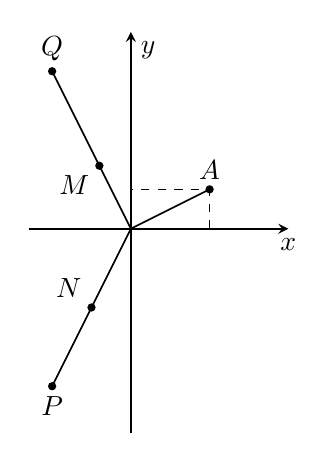
\begin{tikzpicture}[>=stealth, scale= 1,color=black,line width=0.6pt,xscale=1,yscale=1]	
		\draw[->] (-1.3,0) -- (2,0) node[below] { $x$};
		\draw[->] (0,-2.6) -- (0,2.5) node[below right] {$y$};
		\fill (-1,-2) circle (1.5pt); 
		\fill (1,0.5)  circle (1.5pt);
		\fill (-1,2) circle (1.5pt); 
		\fill (-0.4,0.8) circle (1.5pt);
		\fill (-0.5,-1) circle (1.5pt);     
		\draw (-1,-2) node[below]{$P$};
		\draw (1,0.5) node[above]{$A$};
		\draw (-0.5,-1) node[above left]{$N$};
		\draw (-0.4,0.8) node[below left]{$M$};
		\draw (-1,2) node[above]{$Q$};
		\draw[dashed] (1,0)--(1,0.5) --(0,0.5);	
		\draw (0,0)--(1,0.5);	
		\draw (0,0)--(-1,-2);
		\draw (0,0)--(-1,2);	
		\end{tikzpicture}
	}
	\loigiai{
		Gọi $z=x+iy$, $(x, y\in\mathbb{R^+})$ sao cho $x^2+y^2=\dfrac{1}{2}$. Khi đó
		$$w=\dfrac{1}{iz}=\dfrac{1}{-y+xi}=\dfrac{-y-xi}{x^2+y^2}=-2y-2xi.$$
		Dựa vào hình vẽ của đề bài ta suy ra điểm biểu diễn của số phức $w$ là điểm $P$.
	}
\end{ex}

\begin{ex}%[Ngô Quang Anh, 12-EX-1-DCHT]%[2D4B3-2]
	Trên mặt phẳng phức, gọi $M$ là điểm biểu diễn số phức $z=\left(2-3i\right)\cdot\left(1+i\right)$ và $\varphi$ là góc tạo bởi chiều dương trục hoành và véc-tơ $\overrightarrow{OM}$. Tính $\sin 2\varphi$.
	\choice
	{\True $\sin 2\varphi=-\dfrac{5}{13}$}
	{$\sin 2\varphi=\dfrac{5}{13}$}
	{$\sin 2\varphi=\dfrac{13}{5}$}
	{$\sin 2\varphi=-\dfrac{13}{5}$}
	\loigiai{Ta có $z=\left(2-3i\right)\cdot\left(1+i\right)=5-i$ nên $M\left(5;-1\right)\Rightarrow\overrightarrow{OM}=\left(5;-1\right)$.\\
		Do $\tan\varphi=-\dfrac{1}{5}$ nên $\sin 2\varphi=\dfrac{2\tan\varphi}{1+\tan^2\varphi}=-\dfrac{5}{13}$.
	}
\end{ex}

\begin{ex}%[Ngô Quang Anh, 12-EX-1-DCHT]%[2D4B3-2]
	Trên mặt phẳng phức, gọi $M$ là điểm biểu diễn số phức $z=\left(2+i\right)^2\cdot\left(4-i\right)$ và gọi $\varphi$ là góc tạo bởi chiều dương trục hoành và véc-tơ $\overrightarrow{OM}$. Tính $\cos 2\varphi$.
	\choice
	{$\cos 2\varphi=-\dfrac{87}{475}$}
	{$\cos 2\varphi=\dfrac{87}{475}$}
	{$\cos 2\varphi=-\dfrac{87}{425}$}
	{\True $\cos 2\varphi=\dfrac{87}{425}$}
	\loigiai{Ta có $z=\left(2+i\right)^2\cdot\left(4-i\right)=16+13i$ nên $M\left(16;13\right)\Rightarrow\overrightarrow{OM}=\left(16;13\right)$.\\
		Do $\tan\varphi=\dfrac{13}{16}$ nên $\cos 2\varphi=\dfrac{1-\tan^2\varphi}{1+\tan^2\varphi}=\dfrac{87}{425}$.
	}
\end{ex}

\begin{ex}%[Ngô Quang Anh, 12-EX-1-DCHT]%[2D41K-2] 
	Cho $A, B, C, D$ là bốn điểm trong mặt phẳng tọa độ theo thứ tự biểu diễn các số phức $1+2i, 1+\sqrt{3}+i$, $1+\sqrt{3}-i, 1-2i$. Biết $ABCD$ là tứ giác nội tiếp đường tròn tâm $I$, bán kính $R$. Hỏi tọa độ điểm $I$ biểu diễn số phức nào sau đây?
	\choice
	{$z=\sqrt{3}$}
	{$z=1-i\sqrt{3}$}
	{\True $z=1$}
	{$z=-1$}
	\loigiai{Ta có $A\left(1;2\right), B\left(1+\sqrt{3};1\right), C\left(1+\sqrt{3};-1\right), D\left(1;-2\right)$ và gọi $I\left(x;y\right)$.\\
		Do $ABCD$ là tứ giác nội tiếp đường tròn tâm $I$, bán kính $R$ nên $IA=IB=IC=ID=R$. Suy ra:\\
		+) $IA^2=ID^2\Rightarrow \left(x-1\right)^2+\left(y-2\right)^2=\left(x-1\right)^2+\left(y+2\right)^2\Rightarrow y=0$.\\
		+) $IA^2=IB^2\Rightarrow \left(x-1\right)^2+\left(y-2\right)^2=\left(x-1-\sqrt{3}\right)^2+\left(y-1\right)^2$, với $y=0$ ta tìm được $x=1$.\\
		Vậy $I\left(1;0\right)$ nên $I$ biểu diễn số phức $z=1$. 
	}
\end{ex}

\begin{ex}%[Ngô Quang Anh, 12-EX-1-DCHT]%[2D4G4-3]
	Cho hai số phức $z_0, z_1$ khác $0$ thỏa mãn $z_0^2-z_0z_1+z_1^2=0$. Gọi $A, B$ lần lượt là các điểm biểu diễn cho số phức $z_0, z_1$. Hỏi tam giác $OAB$ là tam giác gì?
	\choice
	{\True Tam giác đều}
	{Tam giác vuông tại $O$}
	{Tam giác tù}
	{Tam giác có một góc bằng $45^\circ$}
	\loigiai{ 
		Ta có
		\begin{eqnarray*}
			z_0^2-z_0z_1+z_1^2=0 &\Leftrightarrow & \left(\dfrac{z_0}{z_1}\right)^2-\dfrac{z_0}{z_1}+1=0\\
			&\Leftrightarrow & \hoac{&\dfrac{z_0}{z_1}=\dfrac{1-i\sqrt{3}}{2}\\&\dfrac{z_0}{z_1}=\dfrac{1+i\sqrt{3}}{2}}\\\\
			&\Leftrightarrow & \hoac{&z_0=\dfrac{1-i\sqrt{3}}{2}z_1\\&z_0=\dfrac{1+i\sqrt{3}}{2}z_1.}
		\end{eqnarray*}
		\begin{itemize}
			\item Xét trường hợp $z_0=\dfrac{1-i\sqrt{3}}{2}z_1$.\\
			$OA=\left|z_0\right|=\left|\dfrac{1-i\sqrt{3}}{2}z_1\right|=\left|\dfrac{1-i\sqrt{3}}{2}\right|\cdot \left|z_1\right|=\left|z_1\right|=OB$.\\
			$AB=\left|\overrightarrow{OB}-\overrightarrow{OA}\right|=\left|z_1-z_0\right|=\left|z_1-\dfrac{1-i\sqrt{3}}{2}z_1\right|=\left|\dfrac{1+i\sqrt{3}}{2}z_1\right|=\left|z_1\right|=OB$.\\
			Như vậy: $OA=OB=AB$ $\Rightarrow \triangle OAB$ là tam giác đều.
			\item Xét trường hợp $z_0=\dfrac{1+i\sqrt{3}}{2}z_1$.\\
			$OA=\left|z_0\right|=\left|\dfrac{1+i\sqrt{3}}{2}z_1\right|=\left|\dfrac{1+i\sqrt{3}}{2}\right|\cdot \left|z_1\right|=\left|z_1\right|=OB$.\\
			$AB=\left|\overrightarrow{OB}-\overrightarrow{OA}\right|=\left|z_1-z_0\right|=\left|z_1-\dfrac{1+i\sqrt{3}}{2}z_1\right|=\left|\dfrac{1-i\sqrt{3}}{2}z_1\right|=\left|z_1\right|=OB$.\\
			Như vậy: $OA=OB=AB$ $\Rightarrow \triangle OAB$ là tam giác đều.
		\end{itemize}
		Tóm lại, ba điểm $O$, $A$, $B$ tạo thành tam giác đều ($O$ là gốc tọa độ).
	}
\end{ex}

\begin{ex}%[Ngô Quang Anh, 12-EX-1-DCHT]%[2D4G5-2] 
	Xét số phức $z$ và số phức liên hợp của nó có điểm biểu diễn là $M, M'$. Số phức $z\left(4+3i\right)$ và số phức liên hợp của nó có điểm biểu diễn lần lượt là $N, N'$. Biết rằng $MM'N'N$ là một hình chữ nhật. Tìm giá trị nhỏ nhất của biểu thức $P=\left|z+4i-5\right|$.
	\choice
	{$\min P=\dfrac{5}{\sqrt{34}}$}
	{$\min P=\dfrac{2}{\sqrt{5}}$}
	{\True $\min P=\dfrac{1}{\sqrt{2}}$}
	{$\min P=\dfrac{4}{\sqrt{13}}$}
	\loigiai{ 
		\immini{Đặt $z=a+bi$. Khi đó $z(4+3i)=4a-3b+(3a+4b)i$ và $M(a;b); M'(a;-b), N(4a-3b;3a+4b), N'(4a-3b;-3a-4b)$.\\
			$\vec{MN}=(3a-3b;3a+3b)$. \\
			Theo tính chất đối xứng thì  $MNN'M'$ là hình thang cân. Do đó để $MNN'M'$ là hình chữ nhật thì $\overrightarrow{MN}$ cùng phương với trục $Ox$ hay $3a+3b=0 \Leftrightarrow b=-a$.\\Ta có \begin{eqnarray*}
				|z+4i-5|&=&\sqrt{(a-5)^2+(b+4)^2}\\
				&=& \sqrt{(a-5)^2+(-a+4)^2}=\sqrt{2a^2-18a+ 41}\\
				&=&\sqrt{2\left(a-\dfrac{9}{2} \right)^2+\dfrac{1}{2}}\\
				&\ge &\dfrac{1}{\sqrt{2}}.
		\end{eqnarray*}}{
			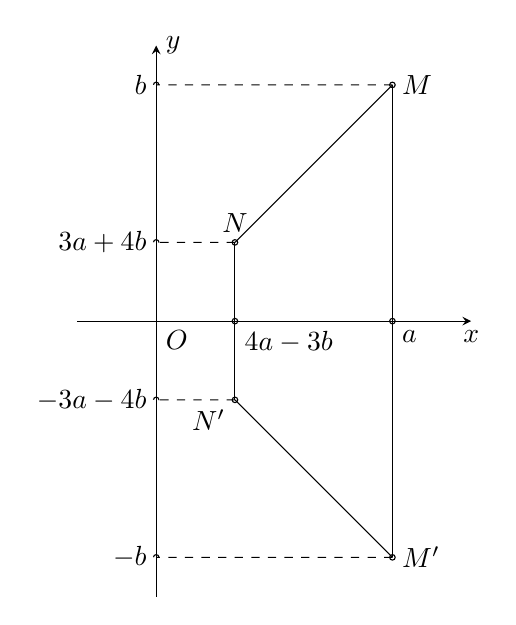
\begin{tikzpicture}[>=stealth]
			\draw[->] (-1,0)--(0,0) node[below right]{$O$}--(4,0) node[below]{$x$};
			\draw[->] (0,-3.5) --(0,3.5) node[right]{$y$};
			\draw (3,3) node[right]{$M$} circle (1pt);
			\draw (3,-3) node[right]{$M'$} circle (1pt);
			\draw (1,1) node[above]{$N$} circle (1pt);
			\draw (1,-1) node[below left]{$N'$} circle (1pt);
			\draw (1,0) node[below right]{$4a-3b$} circle (1pt);
			\draw (3,0) node[below right]{$a$} circle (1pt);
			\draw (1,1)--(1,-1);
			\draw (1,1)--(3,3);
			\draw (1,-1)--(3,-3);
			\draw (3,3)--(3,-3);
			\draw[dashed] (3,3)--(0,3) node[left]{$b$}circle (1pt);
			\draw[dashed] (3,-3)--(0,-3) node[left]{$-b$}circle (1pt);
			\draw[dashed] (1,1)--(0,1) node[left]{$3a+4b$}circle (1pt);
			\draw[dashed] (1,-1)--(0,-1) node[left]{$-3a-4b$}circle (1pt);
			\end{tikzpicture}
		}
		\noindent	Dấu bằng xảy ra khi và chỉ khi $a=\dfrac{9}{2}$ hay $z=\dfrac{9}{2}-\dfrac{9}{2}i$.\\
		Vậy giá trị nhỏ nhất của $|z+4i-5|$ bằng  $\dfrac{1}{\sqrt{2}}$ khi và chỉ khi $z=\dfrac{9}{2}-\dfrac{9}{2}i$.
	}
\end{ex}

\begin{ex}%[Ngô Quang Anh, 12-EX-1-DCHT]%[2D4K2-1] 
	Cho hai số phức $z_1, z_2$ thỏa mãn $\left|z_1\right|=2, \left|z_2\right|=\sqrt{3}$ và nếu gọi $M, N$ lần lượt là điểm biểu diễn của $z_1, iz_2$ thì $\widehat{MON}=30^\circ$. Tính $P=\left|z_1^2+4z_2^2\right|$.
	\choice
	{$P=\sqrt{5}$}
	{\True $P=4\sqrt{7}$}
	{$P=3\sqrt{3}$}
	{$P=5\sqrt{2}$}
	\loigiai{ 
		Ta có $z_1^2+4z_2^2 = z_1^2 - (2iz_2)^2 = (z_1-2iz_2)(z_1+2iz_2)$.\\
		Lại có $\left(\overrightarrow{OM}, \overrightarrow{ON}\right)=30^\circ$ và $|z_1^2+4z_2^2|=|(z_1-2iz_2)(z_1+2iz_2)| = |z_1-2iz_2| \cdot |z_1+2iz_2|$.\\
		Mặt khác
		\allowdisplaybreaks
		\begin{eqnarray*}
			&& |z_1-2iz_2|^2 = |z_1|^2 + 4|iz_2|^2 - 4|z_1||iz_2|\cos 30^\circ = 2^2+4\cdot (\sqrt{3})^2 - 4\cdot 2 \cdot \sqrt{3} \cdot \dfrac{\sqrt{3}}{2} = 4.\\
			&& |z_1+2iz_2|^2 = |z_1|^2 + 4|iz_2|^2 + 4|z_1||iz_2|\cos 30^\circ = 2^2+4\cdot (\sqrt{3})^2 + 4\cdot 2 \cdot \sqrt{3} \cdot \dfrac{\sqrt{3}}{2} = 28.
		\end{eqnarray*}
		Do đó $\left|z_1^2 + 4z_2^2\right| = \sqrt{4\cdot28}= 4\sqrt{7}$.	
	}
\end{ex}

\begin{dang}{Tập hợp điểm của số phức là đường thẳng và các bài toán liên quan}	
\end{dang}
\begin{bt}%[Đỗ Đường Hiếu, dự án (12-EX-1-DCDH(L1))]%[2D4K3-4]
	\begin{listEX}[1]
		\item Cho số phức $z$ thỏa mãn $\left|z-(1+i)\right|=\left|z+2i\right|$. Tập hợp các điểm biểu diễn số phức $w=(3-4i)z-1$ trên mặt phẳng tọa độ là một đường thẳng. Viết phương trình đường thẳng đó. \dapso{$3x+y+8=0$}
		\loigiai{Gọi $M(x;y)$ là điểm biểu diễn số phức $w=x+yi$ ($x,y\in\mathbb{R}$). Ta có 
			$$w=(3-4i)z-1=x+yi\Leftrightarrow z=\dfrac{x+1+yi}{3-4i}.$$
			Do đó
			\begin{eqnarray*}
				\left|z-(1+i)\right|=\left|z+2i\right|&\Leftrightarrow& \left|\dfrac{x+1+yi}{3-4i}-(1+i)\right|=\left|\dfrac{x+1+yi}{3-4i}+2i\right|\\
				&\Leftrightarrow& \left|\dfrac{(x-6)+(y+1)i}{3-4i}\right|=\left|\dfrac{(x+9)+(y+6)i}{3-4i}\right|\\
				&\Leftrightarrow& \dfrac{\left|(x-6)+(y+1)i\right|}{\left|3-4i\right|}=\dfrac{\left|(x+9)+(y+6)i\right|}{\left| 3-4i\right|}\\
				&\Leftrightarrow& \left|(x-6)+(y+1)i\right|=\left|(x+9)+(y+6)i\right|\\
				&\Leftrightarrow& \sqrt{(x-6)^2+(y+1)^2}=\sqrt{(x+9)^2+(y+6)^2}\\
				&\Leftrightarrow& (x-6)^2+(y+1)^2=(x+9)^2+(y+6)^2\\
				&\Leftrightarrow& 3x+y+8=0.
			\end{eqnarray*}
			Suy ra, tập hợp các điểm biểu diễn số phức $w$ là đường thẳng có phương trình $3x+y+8=0$.}
		
		\item Cho các số phức $z$ thỏa mãn $\left|z-2-i\right|=\left|\bar{z}+2i\right|$. Tập hợp các điểm biểu diễn số phức $w=(1+i)z-2$ trên mặt phẳng tọa độ là một đường thẳng. Viết phương trình đường thẳng đó. \dapso{$3x+y+5=0$}
		\loigiai{Gọi $M(x;y)$ là điểm biểu diễn số phức $w=x+yi$ ($x,y\in\mathbb{R}$). Ta có 
			$$w=(1+i)z-2=x+yi\Leftrightarrow z=\dfrac{(x+y+2)-(x-y+2)i}{2}.$$
			Do đó
			\begin{eqnarray*}
				\left|z-2-i\right|=\left|\bar{z}+2i\right|&\Leftrightarrow& \left|\dfrac{(x+y+2)-(x-y+2)i}{2}-2-i\right|=\left|\dfrac{(x+y+2)+(x-y+2)i}{2}+2i\right|\\
				&\Leftrightarrow& \left|\dfrac{(x+y-2)-(x-y+4)i}{2}\right|=\left|\dfrac{(x+y+2)+(x-y+6)i}{2}\right|\\
				&\Leftrightarrow& \left|(x+y-2)-(x-y+4)i\right|=\left|(x+y+2)+(x-y+6)i\right|\\
				&\Leftrightarrow& \sqrt{(x+y-2)^2+(x-y+4)^2}=\sqrt{(x+y+2)^2+(x-y+6)^2}\\
				&\Leftrightarrow& (x+y-2)^2+(x-y+4)^2=(x+y+2)^2+(x-y+6)^2\\
				&\Leftrightarrow& 3x+y+5=0.
			\end{eqnarray*}
			Suy ra, tập hợp các điểm biểu diễn số phức $w$ là đường thẳng có phương trình $3x+y+5=0$.}
	\end{listEX}
\end{bt}

\begin{bt}%[Đỗ Đường Hiếu, dự án (12-EX-1-DCDH(L1))]%[2D4B2-4]
	Cho số phức $z$ thỏa mãn  $2\left|z-2+3i\right|=\left|2i-1-2\bar{z}\right|$. Tập hợp các điểm $M$ biểu diễn số phức $z$ trong mặt phẳng tọa độ $Oxy$ là đường thẳng có phương trình nào sau đây?
	\choice
	{\True $20x-16y-47=0$}
	{$20x+16y-47=0$}
	{$20x-16y+47=0$}
	{$20x+16y+47=0$}
	\loigiai{Gọi $M(x;y)$ là điểm biểu diễn số phức $z=x+yi$ ($x,y\in\mathbb{R}$). Ta có 
		\begin{eqnarray*}
			&& 2\left|z-2+3i\right|=\left|2i-1-2\bar{z}\right|\\
			&\Leftrightarrow &2\left|(x+yi)-2+3i\right|=\left|2i-1-2(x-yi)\right|\\
			&\Leftrightarrow &2\left|(x-2)+(y+3)i\right|=\left|(-2x-1)+(2y+2)i\right|\\
			&\Leftrightarrow & 2\sqrt{(x-2)^2+(y+3)^2}=\sqrt{(-2x-1)^2+(2y+2)^2}\\
			&\Leftrightarrow & 4\left[(x-2)^2+(y+3)^2\right] =(-2x-1)^2+(2y+2)^2\\
			&\Leftrightarrow & 20x-16y-47=0.
		\end{eqnarray*}
		Suy ra, tập hợp các điểm biểu diễn số phức $z$ là đường thẳng có phương trình $20x-16y-47=0$.
	}
\end{bt}

\begin{ex}%[Đỗ Đường Hiếu, dự án (12-EX-1-DCDH(L1))]%[2D4B2-4]
	Tìm tập hợp điểm biểu diễn số phức $z$ thỏa mãn  $\left|z\right|=\left|\bar{z}-2+3i\right|$. 
	\choice
	{Đường thẳng $d\colon 4x-6y+13=0$}
	{\True Đường thẳng $d\colon 4x+6y-13=0$}
	{Đường thẳng $d\colon 6x-4y-13=0$}
	{Đường thẳng $d\colon 6x-4y+13=0$}
	\loigiai{Gọi $M(x;y)$ là điểm biểu diễn số phức $z=x+yi$  ($x,y\in\mathbb{R}$). Ta có 
		\begin{eqnarray*}
			&& \left|z\right|=\left|\bar{z}-2+3i\right|\\
			&\Leftrightarrow &\left|x+yi\right|=\left|(x-yi)-2+3i\right|\\
			&\Leftrightarrow &\left|x+yi\right|=\left|(x-2)+(3-y)i\right|\\
			&\Leftrightarrow & \sqrt{x^2+y^2}=\sqrt{(x-2)^2+(3-y)^2}\\
			&\Leftrightarrow & x^2+y^2 =(x-2)^2+(3-y)^2\\
			&\Leftrightarrow &4x+6y-13=0.
		\end{eqnarray*}
		Suy ra tập hợp các điểm biểu diễn số phức $z$ là đường thẳng có phương trình $4x+6y-13=0$.}
\end{ex}


\begin{ex}%[Đỗ Đường Hiếu, dự án (12-EX-1-DCDH(L1))]%[2D4B2-4]
	Trong mặt phẳng tọa độ $Oxy$, tìm tập hợp các điểm biểu diễn số phức $z$ thỏa mãn $z(1+i)$ là số thực. 
	\choice
	{Trục $Oy$}
	{Trục $Oz$}
	{\True $y=-x$}
	{$y=x$}
	\loigiai{Gọi $M(x;y)$ là điểm biểu diễn số phức $z=x+yi$ $(x,y\in\mathbb{R})$. Ta có $z(1+i)=(x+yi)(1+i)=(x-y)+(x+y)i$.\\
		Để $z(1+i)$ là số thực điều kiện cần và đủ là $x+y=0\Leftrightarrow y=-x$.\\
		Suy ra, tập hợp các điểm biểu diễn số phức $z$ là đường thẳng có phương trình $y=-x$.}
\end{ex}


\begin{ex}%[Đỗ Đường Hiếu, dự án (12-EX-1-DCDH(L1))]%[2D4B2-4]
	Trong mặt phẳng tọa độ $Oxy$, tìm tập hợp các điểm biểu diễn số phức $z$ thỏa mãn điều kiện $w=z(2+3i)+5-i$ là số thuần ảo. 
	\choice
	{Đường thẳng $2x-3y+1=0$}
	{\True Đường thẳng $2x-3y+5=0$}
	{Đường thẳng $3x+2y+1=0$}
	{Đường thẳng $3x+2y-1=0$}
	\loigiai{Gọi $M(x;y)$ là điểm biểu diễn số phức $z=x+yi$ ($x,y\in\mathbb{R}$). Ta có 
		$$ w=z(2+3i)+5-i=(x+yi)(2+3i)+5-i=(2x-3y+5)+(3x+2y-1)i. $$
		Để $w=z(2+3i)+5-i$ là số thuần ảo điều kiện cần và đủ là $2x-3y+5=0$.\\
		Suy ra, tập hợp các điểm biểu diễn số phức $z$ là đường thẳng có phương trình $2x-3y+5=0$.}
\end{ex}


\begin{ex}%[Đỗ Đường Hiếu, dự án (12-EX-1-DCDH(L1))]%[2D4B2-4]
	Tìm tất cả các số phức $z$ thỏa mãn $\left|z-2i\right|=\sqrt{5}$ và điểm biểu diễn số phức $z$ thuộc đường thẳng $d\colon 3x-y+1=0$. 
	\choice
	{$z=1-4i$}
	{\True $z=1+4i$ hoặc $z=-\dfrac{2}{5}-\dfrac{1}{5}i$}
	{$z=-1-2i$ hoặc $z=\dfrac{2}{5}+\dfrac{11}{5}i$}
	{$z=-\dfrac{2}{5}+\dfrac{1}{5}i$}
	\loigiai{Gọi $M(x;y)$ là điểm biểu diễn số phức $z=x+yi$ ($x,y\in\mathbb{R}$). Ta có 
		\begin{eqnarray*}
			\left|z-2i\right|=\sqrt{5}&\Leftrightarrow & \left|(x+yi)-2i\right|=\sqrt{5}\\
			&\Leftrightarrow &\left|x+(y-2)i\right|=\sqrt{5}\\
			&\Leftrightarrow & x^2+(y-2)^2=5.
		\end{eqnarray*}
		Mặt khác, điểm biểu diễn số phức $z$ thuộc đường thẳng $d\colon 3x-y+1=0$ nên ta có hệ phương trình
		\begin{eqnarray*}
			\heva{&x^2+(y-2)^2=5\\&3x-y+1=0}&\Leftrightarrow & \heva{&x=1\\&y=4}\;\text{hoặc}\;\heva{&x=-\dfrac{2}{5}\\&y=-\dfrac{1}{5}.}
		\end{eqnarray*}
		Từ đó suy ra $z=1+4i$ hoặc $z=-\dfrac{2}{5}-\dfrac{1}{5}i$.
	}
\end{ex}




\begin{ex}%[Đỗ Đường Hiếu, dự án (12-EX-1-DCDH(L1))]%[2D4B3-4]
	Cho số phức $z$ thỏa mãn $\left|z-i\right|=\left|z-1+2i\right|$. Tập hợp các điểm biểu diễn số phức $w=(2-i)z+1$ trên mặt phẳng tọa độ là một đường thẳng. Viết phương trình đường thẳng đó.
	\choice
	{$x-7y-9=0$}
	{$x+7y-9=0$}
	{\True $x+7y+9=0$}
	{$x-7y+9=0$}
	\loigiai{Gọi $M(x;y)$ là điểm biểu diễn số phức $w=x+yi$ ($x,\,y\in\mathbb{R}$) thỏa bài toán.\\
		Ta có $w=(2-i)z+1=x+yi\Leftrightarrow z=\dfrac{x-1+yi}{2-i}$.\\
		Từ đó
		\begin{eqnarray*}
			\left|z-i\right|=\left|z-1+2i\right|&\Leftrightarrow & \left|\dfrac{x-1+yi}{2-i}-i\right|=\left|\dfrac{x-1+yi}{2-i}-1+2i\right|\\
			&\Leftrightarrow & \dfrac{\left|(x-2)+(y-2)i\right|}{\left|2-i\right|}=\dfrac{\left|(x-1)+(y+5)i\right|}{\left|2-i\right|}\\
			&\Leftrightarrow &\sqrt{(x-2)^2+(y-2)^2}=\sqrt{(x-1)^2+(y+5)^2}\\
			&\Leftrightarrow & x+7y+9=0.
		\end{eqnarray*}
	}
\end{ex}

\begin{nx}
	Bài toán cho $z$, yêu cầu tìm tập hợp điểm biểu diễn $w$ (loại gián tiếp) thường ta sẽ gọi $w=x+yi$, sau đó biểu thị $z$ theo $x$, $y$ sẽ tìm được tập hợp điểm.
\end{nx}


\begin{ex}%[Đỗ Đường Hiếu, dự án (12-EX-1-DCDH(L1))]%[2D4B2-4]
	Cho tất cả các số phức $z=x+yi$ ($x,\,y\in\mathbb{R}$) thỏa mãn $\left|z+2i-1\right|=\left|z+i\right|$. Biết $z$ được biểu diễn bởi điểm $M$ sao cho $MA$ ngắn nhất với $A(1;3)$. Tìm $P=2x+3y$.
	\choice
	{\True $P=9$}
	{$P=11$}
	{$P=-3$}
	{$P=5$}
	\loigiai{Gọi $M(x;y)$ là điểm biểu diễn số phức $z=x+yi$ ($x,y\in\mathbb{R}$). Ta có 
		\begin{eqnarray*}
			\left|z+2i-1\right|=\left|z+i\right|&\Leftrightarrow & \left|x+yi+2i-1\right|=\left|x+yi+i\right|\\
			&\Leftrightarrow & \left|(x-1)+(y+2)i\right|=\left|x+(y+1)i\right|\\
			&\Leftrightarrow &  (x-1)^2+(y+2)^2=x^2+(y+1)^2\\
			&\Leftrightarrow &  x-y-2=0.			
		\end{eqnarray*}	
		Như vậy, tập hợp các điểm biểu diễn số phức $z$ là đường thẳng $\Delta\colon x-y-2=0$. Gọi $H$ là hình chiếu vuông góc của điểm $A(1;3)$ trên đường thẳng $\Delta$,khi đó $H(3;1)$.\\
		Ta luôn có $MA\ge MH$. Nên, $MA$ ngắn nhất khi và chỉ khi $M\equiv H$, hay $M(3;1)$.\\
		Do đó $P=2x+3y=2\cdot 3+3\cdot 1=9$.}
\end{ex}	


\begin{ex}%[Đỗ Đường Hiếu, dự án (12-EX-1-DCDH(L1))]%[2D4B5-2]
	Cho hai số phức $z_1=1+3i$ và $z_2=-5-3i$. Tìm điểm $M(x;y)$ biểu diễn số phức $z_3$, biết rằng trong mặt phẳng phức điểm $M$ nằm trên đường thẳng $x-2y+1=0$ và mô-đun số phức $w=3z_3-z_2-2z_1$ đạt giá trị nhỏ nhất.
	\choice
	{$M\left(-\dfrac{3}{5};-\dfrac{1}{5}\right)$}
	{$M\left(\dfrac{3}{5};-\dfrac{1}{5}\right)$}
	{$M\left(\dfrac{3}{5};\dfrac{1}{5}\right)$}
	{\True $M\left(-\dfrac{3}{5};\dfrac{1}{5}\right)$}
	\loigiai{Vì điểm $M(x;y)$ nằm trên đường thẳng $x-2y+1=0$ nên $M=(2y-1;y)$. Do đó $z_3=(2y-1)+yi$.\\
		Ta có $w=3z_3-z_2-2z_1=3\left[(2y-1)+yi\right]-(-5-3i)-2(1+3i)=6y+(3y-3)i$.\\
		$\left|w\right|=\sqrt{(6y)^2+(3y-3)^2}=\sqrt{45\left(y-\dfrac{1}{5}\right)^2+\dfrac{36}{5}}\ge \dfrac{6\sqrt{5}}{5}$.\\
		Đẳng thức xảy ra khi và chỉ khi $y=\dfrac{1}{5}$. \\
		Như vậy $\left|w\right|$ nhỏ nhất khi $M\left(-\dfrac{3}{5};\dfrac{1}{5}\right)$.}
\end{ex}

\begin{dang}{Tập hợp điểm của số phức là đường tròn, hình tròn, hình vành khăn}
\end{dang}

\begin{bt}%[Đỗ Đường Hiếu, dự án (12-EX-1-DCDH(L1))]%[2D4K3-4]
	\begin{enumerate}
		\item Trong mặt phẳng tọa độ $Oxy$, tìm tập hợp những điểm biểu diễn số phức $z$ thỏa mãn điều kiện $\left|z-(3-4i)\right|=2$.
		\dapso{Đường tròn $(C)\colon (x-3)^2+(y+4)^2=4$.}
		\loigiai{Gọi $M(x;y)$ là điểm biểu diễn số phức $z=x+yi$ ($x,\,y\in\mathbb{R}$) thỏa mãn bài toán.\\
			Ta có
			\begin{eqnarray*}
				\left|z-(3-4i)\right|=2&\Leftrightarrow & \left|x+yi-(3-4i)\right|=2\\
				&\Leftrightarrow & \left|(x-3)+(y+4)i\right|=2\\
				&\Leftrightarrow & \sqrt{(x-3)^2+(y+4)^2}=2\\
				&\Leftrightarrow & (x-3)^2+(y+4)^2=4.
			\end{eqnarray*} 
			Vậy, tập hợp các điểm $M(x;y)$ là điểm biểu diễn số phức $z$ thỏa mãn bài toán là đường tròn  $(C)\colon (x-3)^2+(y+4)^2=4$ có tâm $I(3;-4)$, bán kính $R=2$.}
		\item Cho số phức $z$ thỏa mãn $\left|z+2\right|=5$. Biết rằng tập hợp điểm biểu diễn của số phức $w=(1-2i)z+3$ là một đường tròn tâm $I$ và bán kính $R$. Tìm $I$ và $R$.
		\dapso{$I(1;4)$, $R=5\sqrt{5}$.}
		\loigiai{Gọi $w=x+yi$ ($x,\,y\in\mathbb{R}$). Theo đề bài ta có
			\begin{eqnarray*}
				w=(1-2i)z+3&\Leftrightarrow &z=\dfrac{w-3}{1-2i}\\
				&\Leftrightarrow &z+2=\dfrac{w-3}{1-2i}+2\\
				&\Leftrightarrow &z+2=\dfrac{w-1-4i}{1-2i}\\
				&\Leftrightarrow &z+2=\dfrac{(x-1)+(y-4)i}{1-2i}.
			\end{eqnarray*}
			Lấy mô-đun hai vế ta được
			\begin{eqnarray*}
				&&\left|z+2\right| =\left| \dfrac{(x-1)+(y-4)i}{1-2i}\right| \\
				&\Leftrightarrow & 5=\dfrac{\left| (x-1)+(y-4)i\right| }{\left| 1-2i\right| }\\
				&\Leftrightarrow & 5=\dfrac{\sqrt{(x-1)^2+(y-4)^2} }{\sqrt{5}}\\
				&\Leftrightarrow & (x-1)^2+(y-4)^2=(5\sqrt{5})^2.
			\end{eqnarray*}
			Vậy, tập hợp các điểm biểu diễn số phức $w$ là đường tròn có tâm $I(1;4)$, bán kính $R=5\sqrt{5}$.}
		\item Cho số phức $z$ thỏa mãn $(2+i)\left|z\right| = \dfrac{\sqrt{10}}{z}+1-2i$. Biết tập hợp điểm biểu diễn của số phức $w=(3-4i)z-1+2i$ là một đường tròn tâm $I$ và bán kính $R$. Tìm $I$ và $R$.
		\dapso{$I(-1;2)$, $R=5$.}
		\loigiai{Ta có
			$(2+i)\left|z\right| = \dfrac{\sqrt{10}}{z}+1-2i\Leftrightarrow \left(2\left|z\right| -1\right)+\left(\left|z\right| +2\right)i=\dfrac{\sqrt{10}}{z}$.\\
			Lấy mô-đun hai vế, ta có
			\begin{eqnarray*}
				&&\left| \left(2\left|z\right| -1\right)+\left(\left|z\right| +2\right)i\right| =\left| \dfrac{\sqrt{10}}{z}\right| \\
				&\Leftrightarrow &  \sqrt{\left(2\left|z\right| -1\right)^2+\left(\left|z\right| +2\right)^2}=\dfrac{\sqrt{10}}{\left|z\right|}\\
				&\Leftrightarrow &  5\left|z\right|^2+5=\dfrac{10}{\left|z\right|^2}\\
				&\Leftrightarrow & 5\left|z\right|^4+5\left|z\right|^2-1=0\Leftrightarrow \left|z\right|=1.
			\end{eqnarray*}
			Gọi $w=x+yi$ ($x,\,y\in\mathbb{R}$). Theo đề bài ta có
			$$w=(3-4i)z-1+2i\Leftrightarrow z=\dfrac{w+1-2i}{3-4i}\Leftrightarrow z=\dfrac{(x+1)+(y-2)i}{3-4i}.$$
			Lấy mô-đun hai vế ta được
			\begin{eqnarray*}
				\left| z\right| =\left|\dfrac{(x+1)+(y-2)i}{3-4i}\right| &\Leftrightarrow & \left|z\right|=\dfrac{\left|(x+1)+(y-2)i\right|}{\left|3-4i\right|}\\
				&\Leftrightarrow & 1=\dfrac{\sqrt{(x+1)^2+(y-2)^2}}{5}\\
				&\Leftrightarrow & (x+1)^2+(y-2)^2 =25.
			\end{eqnarray*}
			Vậy, tập hợp điểm biểu diễn số phức $w$ là đường tròn tâm $I(-1;2)$, bán kính $R=5$.}
		\item Hãy xác định tập hợp các điểm trong mặt phẳng phức biểu diễn các số phức $z$ thỏa mãn $1<\left|z-1\right| <2$.
		\loigiai{\immini{Gọi $M(x;y)$ là điểm biểu diễn số phức $z=x+yi$ ($x,\,y\in\mathbb{R}$) thỏa mãn bài toán.\\
				Theo đề bài ta có 
				\begin{eqnarray*}
					1<\left|z-1\right|<2 &\Leftrightarrow & 1<\left|(x-1)+yi\right|<2\\
					&\Leftrightarrow & 1<\sqrt{(x-1)^2+y^2}<2\\
					&\Leftrightarrow & 1<(x-1)^2+y^2<4.
				\end{eqnarray*}
				Vậy tập hợp các điểm $M(x;y)$ biểu diễn số phức $z$ thỏa mãn $1<\left|z-1\right| <2$ là hình vành khăn là phần nằm giữa hai đường tròn đồng tâm $I(1;0)$ với bán kính $R_1=1$, $R_2=2$ như hình vẽ bên (không tính những điểm nằm trên hai đường tròn).}
			{\begin{tikzpicture}[>=stealth,x=1 ,y=1 ,scale=1]
				\draw[->] (-1.5,0) -- (3.5,0) node[below] {$x$};
				\draw[->] (0,-2.5) -- (0,2.5) node[above] {$y$};
				\filldraw (0,0) circle (1pt)node[below right]{$O$};
				
				\draw[domain=0:2,samples=200] plot (\x,{sqrt(1-(\x-1)^2)});
				\draw[domain=0:2,samples=200] plot (\x,{-sqrt(1-(\x-1)^2)});
				\draw[domain=-1:3,samples=200] plot (\x,{sqrt(4-(\x-1)^2)});
				\draw[domain=-1:3,samples=200] plot (\x,{-sqrt(4-(\x-1)^2)});
				
				\fill [pattern = north east lines, line width = 2pt,draw =none]plot[domain=-1:3](\x,{sqrt(4-(\x-1)^2)})--(3,0)--(2,0)--plot[domain=2:0](\x,{sqrt(1-(\x-1)^2)})--(0,0)--(-1,0)-- cycle;
				\fill [pattern = north east lines, line width = 2pt,draw =none]plot[domain=-1:3](\x,{-sqrt(4-(\x-1)^2)})--(3,0)--(2,0)--plot[domain=2:0](\x,{-sqrt(1-(\x-1)^2)})--(0,0)--(-1,0)-- cycle;
				\filldraw (1,0) circle (1pt)node[below]{$I$};
				\foreach \x in {-1,1,2,3} \filldraw (\x,0) circle (1pt);
				\end{tikzpicture}}}
	\end{enumerate}
\end{bt}



\begin{ex}%[Đỗ Đường Hiếu, dự án (12-EX-1-DCDH(L1))]%[2D4K2-4]
	Trong mặt phẳng tọa độ $Oxy$, tìm tập hợp những điểm biểu diễn số phức $z$ thỏa mãn điều kiện $\left|z-i\right|=\left|(1+i)z\right|$. 
	\choice
	{$x^2+(y-1)^2=4$}
	{$(x-1)^2+y^2=4$}
	{\True $x^2+(y+1)^2=2$}
	{$(x+1)^2+y^2=2$}
	\loigiai{Gọi $M(x;y)$ là điểm biểu diễn số phức $z=x+yi$ ($x,y\in\mathbb{R}$). Ta có 
		\begin{eqnarray*}
			\left|z-i\right|=\left|(1+i)z\right| &\Leftrightarrow & \left|(x+yi)-i\right|=\left|(1+i)(x+yi)\right|\\
			&\Leftrightarrow & \left|x+(y-1)i\right|=\left|(x-y)+(x+y)i\right|\\
			&\Leftrightarrow & \sqrt{x^2+(y-1)^2}=\sqrt{(x-y)^2+(x+y)^2}\\
			&\Leftrightarrow & x^2+(y-1)^2=(x-y)^2+(x+y)^2\\
			&\Leftrightarrow & x^2+y^2+2y-1=0\\
			&\Leftrightarrow & x^2+(y+1)^2=2.
		\end{eqnarray*}
		Vậy,  tập hợp những điểm biểu diễn số phức $z$ thỏa mãn điều kiện $\left|z-i\right|=\left|(1+i)z\right|$ là đường tròn $(C)$ có phương trình $x^2+(y+1)^2=2$.}
\end{ex}		

\begin{note}
	Cần nhớ những kiến thức cơ bản về đường tròn trong mặt phẳng tọa độ $Oxy$.
	\begin{enumerate}
		\item Để viết phương trình đường tròn ta cần tìm tâm $I(a; b)$ và bán kính $R$. 
		\begin{itemize}
			\item[Dạng 1] Đường tròn $(C)$ có phương trình $(x-a)^2+(y-b)^2=R^2$.
			\item[Dạng 2] Đường tròn $(C)$ có phương trình $x^2+y^2-2ax-2by+c=0$, với $R=\sqrt{a^2+b^2-c}$.
		\end{itemize}
		\item Chu vi đường tròn $p=2\pi R$ và diện tích hình tròn $S=\pi R^2$.
	\end{enumerate}
	
\end{note}


\begin{ex}%[Đỗ Đường Hiếu, dự án (12-EX-1-DCDH(L1))]%[2D4B2-4]
	Trong mặt phẳng phức, tập hợp các điểm biểu diễn số phức $z$ thỏa mãn $\left|z-3+5i\right|=4$ là một đường tròn. Tính chu vi $p$ của đường tròn đó.
	\choice
	{$p=4\pi$}
	{$p=2\pi$}
	{\True $p=8\pi$}
	{$p=16\pi$}
	\loigiai{Tập hợp các điểm biểu diễn số phức $z$ thỏa mãn $\left|z-3+5i\right|=4$ là đường tròn tâm $I(3;-5)$, bán kính $R=4$. Chu vi đường tròn là $p=2\pi R=8\pi$.}
\end{ex}		


\begin{ex}%[Đỗ Đường Hiếu, dự án (12-EX-1-DCDH(L1))]%[2D4B2-4]
	Cho số phức $z$ thỏa mãn $(z+1)(\bar{z}-2i)$ là một số thuần ảo. Tập hợp điểm biểu diễn số phức $z$ là một đường tròn có diện tích $S$ bằng bao nhiêu?
	\choice
	{$S=5\pi$}
	{\True $S=\dfrac{5\pi}{4}$}
	{$S=\dfrac{5\pi}{2}$}
	{$S=25\pi$}
	\loigiai{Gọi $M(x;y)$ là điểm biểu diễn số phức $z=x+yi$ ($x,y\in\mathbb{R}$). \\
		Ta có $(z+1)(\bar{z}-2i)=(x+yi+1)(x-yi-2i)=\left[(x+1)+yi\right]\cdot \left[x-(y+2)i\right]=(x^2+y^2+x+2y)-(2x+y+2)i$.\\
		$(z+1)(\bar{z}-2i)$ là một số thuần ảo khi và chỉ khi $x^2+y^2+x+2y=0\Leftrightarrow \left(x+\dfrac{1}{2}\right)^2+(y+1)^2=\dfrac{5}{4}$.\\
		Suy ra, tập hợp các điểm biểu diễn số phức $z$ là đường tròn $(C)$ tâm $I\left(-\dfrac{1}{2};-1\right)$, bán kính $R=\dfrac{\sqrt{5}}{2}$.\\
		Diện tích hình tròn $(C)$ là $S=\pi R^2=\dfrac{5\pi}{4}$.}
\end{ex}	


\begin{ex}%[Đỗ Đường Hiếu, dự án (12-EX-1-DCDH(L1))]%[2D4B2-4]
	Cho số phức $z$ thỏa mãn $\left|z-1\right|=2$. Biết rằng tập hợp điểm biểu diễn số phức $w=2z-i$ là một đường tròn tâm $I$ và bán kính $R$. Tìm khẳng định \textbf{đúng}.
	\choice
	{$I(2;-1)$, $R=2$}
	{$I(2;1)$, $R=4$}
	{\True $I(2;-1)$, $R=4$}
	{$I(-2;1)$, $R=2$}
	\loigiai{Gọi $w=x+yi$ ($x,\,y\in\mathbb{R}$). Theo đề bài ta có
		\begin{eqnarray*}
			w=2z-i&\Leftrightarrow &z=\dfrac{w+i}{2}\\
			&\Leftrightarrow &z-1=\dfrac{w+i}{2}-1\\
			&\Leftrightarrow &z-1=\dfrac{w-2+i}{2}\\
			&\Leftrightarrow &z-1=\dfrac{(x-2)+(y+1)i}{2}.
		\end{eqnarray*}
		Lấy mô-đun hai vế ta được
		\begin{eqnarray*}
			&&\left|z-1\right| =\left| \dfrac{(x-2)+(y+1)i}{2}\right| \\
			&\Leftrightarrow & 2=\dfrac{\left| (x-2)+(y+1)i\right|}{2}\\
			&\Leftrightarrow & 2=\dfrac{\sqrt{(x-2)^2+(y+1)^2}}{2}\\
			&\Leftrightarrow & (x-2)^2+(y+1)^2=16.
		\end{eqnarray*}
		Như vậy,tập hợp điểm biểu diễn số phức $w=2z-i$ là một đường tròn tâm $I(2;-1)$ và bán kính $R=4$.}
\end{ex}	



\begin{ex}%[Đỗ Đường Hiếu, dự án (12-EX-1-DCDH(L1))]%[2D4K3-4]
	Cho số phức $z$ thỏa mãn $\left|z-1\right|=1$. Biết rằng tập hợp điểm biểu diễn số phức $w=(1+i\sqrt{3})z+2$ là một đường tròn tâm $I$ và bán kính $R$. Tìm khẳng định \textbf{đúng}.
	\choice
	{$I(3;\sqrt{3})$, $R=4$}
	{\True $I(3;\sqrt{3})$, $R=2$}
	{$I(3;-\sqrt{3})$, $R=4$}
	{$I(-3;\sqrt{3})$, $R=2$}
	\loigiai{Gọi $w=x+yi$ ($x,\,y\in\mathbb{R}$). Theo đề bài ta có
		\begin{eqnarray*}
			w=(1+i\sqrt{3})z+2&\Leftrightarrow &z=\dfrac{w-2}{1+i\sqrt{3}}\\
			&\Leftrightarrow &z-1=\dfrac{w-2}{1+i\sqrt{3}}-1\\
			&\Leftrightarrow &z-1=\dfrac{w-3-i\sqrt{3}}{1+i\sqrt{3}}\\
			&\Leftrightarrow &z-1=\dfrac{(x-3)+(y-\sqrt{3})i}{1+i\sqrt{3}}.
		\end{eqnarray*}
		Lấy mô-đun hai vế ta được
		\begin{eqnarray*}
			&&\left|z-1\right| =\left|\dfrac{(x-3)+(y-\sqrt{3})i}{1+i\sqrt{3}}\right| \\
			&\Leftrightarrow & 1=\dfrac{\left|(x-3)+(y-\sqrt{3})i\right|}{\left|1+i\sqrt{3}\right|}\\
			&\Leftrightarrow & 1=\dfrac{\sqrt{(x-3)^2+(y-\sqrt{3})^2}}{2}\\
			&\Leftrightarrow & (x-3)^2+(y-\sqrt{3})^2=4.
		\end{eqnarray*}
		Như vậy,tập hợp điểm biểu diễn số phức $w=(1+i\sqrt{3})z+2$ là một đường tròn tâm $I(3;\sqrt{3})$ và bán kính $R=2$.}
\end{ex}		



\begin{ex}%[Đỗ Đường Hiếu, dự án (12-EX-1-DCDH(L1))]%[2D4K2-4]
	Cho số phức $z$ thỏa mãn $\left|z-1+2i\right|=3$. Biết tập hợp điểm biểu diễn số phức $w=\bar{z}+1-i$ là một đường tròn tâm $I$ và bán kính $R$. Tìm khẳng định \textbf{đúng}.
	\choice
	{\True $I(2;1)$, $R=3$}
	{$I(1;2)$, $R=\sqrt{3}$}
	{$I(2;1)$, $R=4$}
	{$I(1;2)$, $R=5$}
	\loigiai{Gọi $w=x+yi$ ($x,\,y\in\mathbb{R}$). Theo đề bài ta có
		\begin{eqnarray*}
			w=\bar{z}+1-i&\Leftrightarrow &\bar{z}=w-1+i\\
			&\Leftrightarrow &\bar{z}=(x-1)+(y+1)i\\
			&\Leftrightarrow &z=(x-1)-(y+1)i\\
			&\Leftrightarrow &z-1+2i=(x-1)-(y+1)i-1+2i\\
			&\Leftrightarrow &z-1+2i=(x-2)+(1-y)i.
		\end{eqnarray*}
		Lấy mô-đun hai vế ta được
		\begin{eqnarray*}
			&&\left|z-1+2i\right| =\left|(x-2)+(1-y)i\right| \\
			&\Leftrightarrow & 3=\sqrt{(x-2)^2+(1-y)^2}\\
			&\Leftrightarrow & (x-2)^2+(y-1)^2=9.
		\end{eqnarray*}
		Vậy, tập hợp điểm biểu diễn số phức $w=\bar{z}+1-i$ là một đường tròn tâm $I(2;1)$ và bán kính $R=3$.}
\end{ex}


\begin{ex}%[Đỗ Đường Hiếu, dự án (12-EX-1-DCDH(L1))]%[2D4K3-4]
	Cho số phức $z$ thỏa mãn $\left|z+1\right|^2=\dfrac{z\bar{z}}{2}$. Biết rằng tập hợp điểm biểu diễn số phức $w=(1+2i)z+1$ là một đường tròn tâm $I$ và bán kính $R$. Tìm $I$ và $R$.
	\choice
	{$I(0;-2)$, $R=\sqrt{5}$}
	{$I(1;-4)$, $R=\sqrt{10}$}
	{$I(0;2)$, $R=\sqrt{5}$}
	{\True $I(-1;-4)$, $R=\sqrt{10}$}
	\loigiai{Gọi $w=x+yi$ ($x,\,y\in\mathbb{R}$). Theo đề bài ta có
		\begin{eqnarray*}
			w=(1+2i)z+1 &\Leftrightarrow &z=\dfrac{w-1}{1+2i}\\
			&\Leftrightarrow &z=\dfrac{(x-1)+yi}{1+2i}.
		\end{eqnarray*}
		Từ đó ta có 
		\begin{eqnarray*}
			\left|z+1\right|^2=\dfrac{z\bar{z}}{2}&\Leftrightarrow & \left|\dfrac{(x-1)+yi}{1+2i}+1\right|^2=\dfrac{1}{2}\cdot \dfrac{(x-1)+yi}{1+2i}\cdot \dfrac{(x-1)-yi}{1-2i}\\
			&\Leftrightarrow & \left|\dfrac{x+(y+2)i}{1+2i}\right|^2=\dfrac{1}{2}\cdot \dfrac{(x-1)^2+y^2}{5}\\
			&\Leftrightarrow & \dfrac{x^2+(y+2)^2}{5}=\dfrac{1}{2}\cdot \dfrac{(x-1)^2+y^2}{5}\\
			&\Leftrightarrow & 2\left[x^2+(y+2)^2\right]=(x-1)^2+y^2\\
			&\Leftrightarrow & (x+1)^2+(y+4)^2=10.
		\end{eqnarray*}
		Như vậy,tập hợp điểm biểu diễn số phức $w=(1+2i)z+1$  là một đường tròn tâm $I(-1;-4)$ và bán kính $R=\sqrt{10}$.}
\end{ex}		


\begin{ex}%[Đỗ Đường Hiếu, dự án (12-EX-1-DCDH(L1))]%[2D4K3-4]
	Cho số phức $z$ thỏa mãn $(1-i)\left|\bar{z}\right|=\dfrac{2\sqrt{3}}{z}+1+i$. Biết rằng tập hợp điểm biểu diễn số phức $w=iz-1+i$ là một đường tròn tâm $I$ và bán kính $R$. Tìm khẳng định \textbf{đúng}.
	\choice
	{\True $I(-1;1)$, $R=\sqrt{2}$}
	{$I(1;1)$, $R=\sqrt{2}$}
	{$I(1;1)$, $R=2$}
	{$I(-1;1)$, $R=2$}
	\loigiai{Ta có
		$(1-i)\left|\bar{z}\right|=\dfrac{2\sqrt{3}}{z}+1+i\Leftrightarrow(1-i)\left|z\right|=\dfrac{2\sqrt{3}}{z}+1+i\Leftrightarrow \left(\left|z\right|-1\right)-\left(\left|z\right|+1\right)i=\dfrac{2\sqrt{3}}{z}$.\\
		Lấy mô-đun hai vế, ta có
		\begin{eqnarray*}
			&&\left| \left(\left|z\right|-1\right)-\left(\left|z\right|+1\right)i\right| =\left|\dfrac{2\sqrt{3}}{z}\right| \\
			&\Leftrightarrow &  \sqrt{\left(\left|z\right|-1\right)^2+\left(\left|z\right|+1\right)^2}=\dfrac{2\sqrt{3}}{\left|z\right|}\\
			&\Leftrightarrow &  \left(\left|z\right|-1\right)^2+\left(\left|z\right|+1\right)^2=\dfrac{12}{\left|z\right|^2}\\
			&\Leftrightarrow & \left|z\right|^4+\left|z\right|^2-6=0\\
			&\Rightarrow & \left|z\right|^2=2\\
			&\Rightarrow & \left|z\right|=\sqrt{2}.
		\end{eqnarray*}
		Gọi $w=x+yi$ ($x,\,y\in\mathbb{R}$). Theo đề bài ta có
		$$w=iz-1+i\Leftrightarrow z=-iw-i-1\Leftrightarrow z=(y-1)+(-x-1)i.$$
		Từ đó ta có
		\begin{eqnarray*}
			\left| z\right| =\left|(y-1)+(-x-1)\right| &\Leftrightarrow & \sqrt{2}=\sqrt{(y-1)^2+(-x-1)^2}\\
			&\Leftrightarrow & (x+1)^2+(y-1)^2 =2.
		\end{eqnarray*}
		Vậy, tập hợp điểm biểu diễn số phức $w$ là đường tròn tâm $I(-1;1)$, bán kính $R=\sqrt{2}$.}
\end{ex}


\begin{ex}%[Đỗ Đường Hiếu, dự án (12-EX-1-DCDH(L1))]%[2D4K3-4]
	Cho số phức $z$ thỏa mãn $(3-7i)\left|z\right|=\dfrac{176-82i}{\bar{z}}+7+3i$. Biết tập hợp điểm biểu diễn số phức $w=(1+i)z+2-i$ là một đường tròn tâm $I$ và bán kính $R$. Tìm $I$ và $R$.
	\choice
	{$I(2;-1)$, $R=5$}
	{$I(2;1)$, $R=5$}
	{\True $I(2;-1)$, $R=5\sqrt{2}$}
	{$I(2;1)$, $R=5\sqrt{2}$}
	\loigiai{Ta có
		$(3-7i)\left|z\right|=\dfrac{176-82i}{\bar{z}}+7+3i\Leftrightarrow \left(3\left|z\right|-7\right)-\left(7\left|z\right|+3\right)i=\dfrac{176-82i}{\bar{z}}$.\\
		Lấy mô-đun hai vế, ta có
		\begin{eqnarray*}
			&&\left| \left(3\left|z\right|-7\right)-\left(7\left|z\right|+3\right)i\right| =\left|\dfrac{176-82i}{\bar{z}}\right| \\
			&\Leftrightarrow &  \sqrt{\left(3\left|z\right|-7\right)^2+\left(7\left|z\right|+3\right)^2}=\dfrac{\sqrt{37700}}{\left|z\right|}\\
			&\Leftrightarrow &  \left(3\left|z\right|-7\right)^2+\left(7\left|z\right|+3\right)^2=\dfrac{37700}{\left|z\right|^2}\\
			&\Leftrightarrow & \left|z\right|^4+\left|z\right|^2-650=0\\
			&\Rightarrow & \left|z\right|^2=25\\
			&\Rightarrow & \left|z\right|=5.
		\end{eqnarray*}
		Gọi $w=x+yi$ ($x,\,y\in\mathbb{R}$). Theo đề bài ta có
		$$w=(1+i)z+2-i\Leftrightarrow z=\dfrac{w-2+i}{1+i}\Leftrightarrow z=\dfrac{(x-2)+(y+1)i}{1+i}.$$
		Từ đó ta có
		\begin{eqnarray*}
			&&\left| z\right| =\left|\dfrac{(x-2)+(y+1)i}{1+i}\right| \\
			&\Leftrightarrow &  5=\dfrac{\left|(x-2)+(y+1)i\right|}{\left|1+i\right|}\\
			&\Leftrightarrow &  5=\dfrac{\sqrt{(x-2)^2+(y+1)^2}}{\sqrt{2}}\\
			&\Leftrightarrow & \sqrt{(x-2)^2+(y+1)^2}=5\sqrt{2}\\
			&\Rightarrow &(x-2)^2+(y+1)^2=50.
		\end{eqnarray*}
		Vậy, tập hợp điểm biểu diễn số phức $w$ là đường tròn tâm $I(2;-1)$, bán kính $R=5\sqrt{2}$.}
\end{ex}	


\begin{ex}%[Đỗ Đường Hiếu, dự án (12-EX-1-DCDH(L1))]%[2D4K2-4]
	Cho số phức $z$ thỏa mãn $\left|3z+i\right|^2\le z\cdot \bar{z}+9$. Tìm tập hợp điểm biểu diễn số phức $w$ thỏa mãn $w=\bar{z}+1-i$.
	\choice
	{\True Hình tròn $(x-1)^2+\left(y+\dfrac{5}{8}\right)^2\le \dfrac{73}{64}$}
	{Đường tròn $(x-1)^2+\left(y+\dfrac{5}{8}\right)^2\le \dfrac{73}{64}$}
	{Đường tròn $(x-1)^2+(y+3)^2\le 9$}
	{Hình tròn $(x-1)^2+(y+3)^2\le 9$}
	\loigiai{Gọi $w=x+yi$ ($x,\,y\in\mathbb{R}$). Ta có
		$$w=\bar{z}+1-i\Leftrightarrow \bar{z}=(x-1)+(y+1)i\Leftrightarrow z=(x-1)-(y+1)i.$$
		Từ đó ta có
		\begin{eqnarray*}
			&&\left|3z+i\right|^2\le z\cdot \bar{z}+9\\
			&\Leftrightarrow &  \left|3\left[(x-1)-(y+1)i\right]+i\right|^2\le (x-1)^2+(y+1)^2+9\\
			&\Leftrightarrow &  \left|3(x-1)-(3y+2)i\right|^2\le (x-1)^2+(y+1)^2+9\\
			&\Leftrightarrow & 9(x-1)^2+(3y+2)^2\le (x-1)^2+(y+1)^2+9\\
			&\Leftrightarrow &(x-1)^2+\left(y+\dfrac{5}{8}\right)^2\le \dfrac{73}{64}.
		\end{eqnarray*}
		Vậy, tập hợp điểm biểu diễn số phức $w$ là hình tròn $(x-1)^2+\left(y+\dfrac{5}{8}\right)^2\le \dfrac{73}{64}$.
	}
\end{ex}



\begin{ex}%[Đỗ Đường Hiếu, dự án (12-EX-1-DCDH(L1))]%[2D4K3-4]
	Trong mặt phẳng tọa độ $Oxy$, tìm tập hợp các điểm $M$ biểu diễn số phức $w$ thỏa mãn $w=(1+i\sqrt{3})z+2$ với $\left|z-1\right|\le 2$.
	\choice
	{Hình tròn $x^2+(y-1)^2\le 4$}
	{\True Hình tròn $(x-3)^2+(y-\sqrt{3})^2\le 16$}
	{Hình tròn $x^2+(y-1)^2=16$}
	{Hình tròn $(x-3)^2+(y-\sqrt{3})^2=4$}
	\loigiai{Gọi $w=x+yi$ ($x,\,y\in\mathbb{R}$). Ta có
		$$w=(1+i\sqrt{3})z+2\Leftrightarrow z=\dfrac{w-2}{1+i\sqrt{3}}\Leftrightarrow z=\dfrac{(x-2)+yi}{1+i\sqrt{3}}.$$
		Từ đó ta có
		\begin{eqnarray*}
			&&\left|z-1\right|\le 2\\
			&\Leftrightarrow &  \left|\dfrac{(x-2)+yi}{1+i\sqrt{3}}-1\right|\le 2\\
			&\Leftrightarrow &   \left|\dfrac{(x-3)+(y-\sqrt{3})i}{1+i\sqrt{3}}\right|\le 2\\
			&\Leftrightarrow & \dfrac{\sqrt{(x-3)^2+(y-\sqrt{3})^2}}{2}\le 2\\
			&\Leftrightarrow &(x-3)^2+(y-\sqrt{3})^2\le 16.
		\end{eqnarray*}
		Vậy, tập hợp điểm biểu diễn số phức $w$ là hình tròn $(x-3)^2+(y-\sqrt{3})^2\le 16$.}
\end{ex}


\begin{ex}%[Đỗ Đường Hiếu, dự án (12-EX-1-DCDH(L1))]%[2D4K3-4]
	Tập hợp các điểm biểu diễn số phức $w=(1+i)z+1$ với $z$ là số phức thỏa mãn $\left|z-1\right|\le 1$ là hình tròn. Tính diện tích $S$ của hình tròn đó.
	\choice
	{$S=4\pi$}
	{\True $S=2\pi$}
	{$S=3\pi$}
	{$S=\pi$}
	\loigiai{Gọi $w=x+yi$ ($x,\,y\in\mathbb{R}$). Ta có
		$$w=(1+i)z+1\Leftrightarrow z=\dfrac{w-1}{1+i}\Leftrightarrow z=\dfrac{(x-1)+yi}{1+i}.$$
		Từ đó ta có
		\begin{eqnarray*}
			&&\left|z-1\right|\le 1\\
			&\Leftrightarrow &  \left|\dfrac{(x-1)+yi}{1+i}-1\right|\le 1\\
			&\Leftrightarrow &   \left|\dfrac{(x-1)+yi}{1+i}-1\right|\le 1\\
			&\Leftrightarrow & \dfrac{\sqrt{(x-2)^2+(y-1)^2}}{\sqrt{2}}\le 1\\
			&\Leftrightarrow &x-2)^2+(y-1)^2\le 2.
		\end{eqnarray*}
		Vậy, tập hợp điểm biểu diễn số phức $w$ là hình tròn $(x-2)^2+(y-1)^2\le 2$. Bán kính hình tròn là $R=\sqrt{2}$, diện tích của hình tròn là $S=\pi R^2=2\pi$.}
\end{ex}		



\begin{ex}%[Đỗ Đường Hiếu, dự án (12-EX-1-DCDH(L1))]%[2D4K2-4]
	Trong mặt phẳng tọa độ $Oxy$, tập hợp các điểm $M$ biểu diễn số phức $w$ thỏa mãn $w=\bar{z}+1-i$ với $\left|2z+i\right|^2\le 3z \bar{z}+1$ là một hình tròn. Tìm tâm $I$ và bán kính $R$. 
	\choice
	{$I(1;-1)$, $R=2$}
	{\True $I(1;1)$, $R=2$}
	{$I(-1;-1)$, $R=2$}
	{$I(1;1)$, $R=4$}
	\loigiai{Gọi $w=x+yi$ ($x,\,y\in\mathbb{R}$). Ta có
		$$w=\bar{z}+1-i\Leftrightarrow \bar{z}=w-1+i\Leftrightarrow z=(x-1)-(y+1)i.$$
		Từ đó ta có
		\begin{eqnarray*}
			&&\left|2z+i\right|^2\le 3z \bar{z}+1\\
			&\Leftrightarrow & \left|2\left[(x-1)-(y+1)i\right]+i\right|^2\le 3\left[(x-1)^2+(y+1)^2\right]+1\\
			&\Leftrightarrow &   \left|2(x-1)-(2y+1)i\right|^2\le 3\left[(x-1)^2+(y+1)^2\right]+1\\
			&\Leftrightarrow & 4(x-1)^2+(2y+1)^2\le 3\left[(x-1)^2+(y+1)^2\right]+1\\
			&\Leftrightarrow &(x-1)^2+(y-1)^2\le 4.
		\end{eqnarray*}
		Vậy, tập hợp điểm biểu diễn số phức $w$ là hình tròn có tâm $I(1;1)$ và bán kính $R=2$.}
\end{ex}	

\begin{ex}%[Bùi Quốc Hoàn, dự án (12-EX-1-DCDH(L1))]%[2D4G2-4]
	Trong mặt phẳng phức $Oxy$, tập hợp biểu diễn số phức $z$ thỏa mãn $1\leq \left\vert z + 1 - i\right\vert\leq 2$ là hình vành khăn. Tính chu vi $P$ của hình vành khăn.
	\choice
	{$P = 4\pi$}
	{$P = \pi$}
	{\True $P = 2\pi$}	
	{$P = 3\pi$}		
	%\dotlineans{5}{bt}% luôn ẩn lời giải và hiện 5 dòng kẻ
	\loigiai{
		Giả sử số phức $z$ có dạng $z = x + iy$, với $x$, $y\in\mathbb{R}$.\\
		Khi đó $z + 1 - i =  x + iy + 1 - i = \left(x + 1\right) + \left(y - 1\right)i$.\\
		Do đó $\left\vert z + 1 - i\right\vert = \sqrt{\left(x + 1\right)^2 + \left(y - 1\right)^2}$.\\
		Xét $\left\vert z + 1 - i\right\vert = 2\Leftrightarrow  \sqrt{\left(x + 1\right)^2 + \left(y - 1\right)^2} = 2\Leftrightarrow \left(x + 1\right)^2 + \left(y - 1\right)^2 = 4\quad \left(C_{1}\right)$.\\
		Tương tự ta xét 
		$\left\vert z + 1 - i\right\vert = 1\Leftrightarrow  \sqrt{\left(x + 1\right)^2 + \left(y - 1\right)^2} = 1\Leftrightarrow \left(x + 1\right)^2 + \left(y - 1\right)^2 = 1\quad \left(C_{2}\right)$.\\
		Do đó $P$ là tổng chu vi hai đường tròn $\left(C_{1}\right)$ và $\left(C_{2}\right)$. Mà đường tròn $\left(C_{1}\right)$ có bán kính $R_{1} = 2$ và $\left(C_{2}\right)$ có bán kính $R_{2} = 1$ nên $P = 2\pi\cdot R_{1} - 2\pi\cdot R_{2} =  2\pi\cdot 2  -  2\pi\cdot 1  = 2\pi$. 
	}
	%\dotlinefull{ex}
\end{ex}
\begin{ex}%[Bùi Quốc Hoàn, dự án (12-EX-1-DCDH(L1))]%[2D4K2-4]
	Cho số phức $z$ thỏa mãn điều kiện $3\leq \left\vert z - 3i + 1\right\vert\leq 5$. Tập hợp các điểm biểu diễn số phức $z$ tạo thành một hình phẳng. Tính diện tích $S$ của hình phẳng đó.
	\choice
	{$S = 25\pi$}
	{$S = 8\pi$}
	{$S = 4\pi$}	
	{\True $S = 16\pi$}		
	%\dotlineans{5}{bt}% luôn ẩn lời giải và hiện 5 dòng kẻ
	\loigiai{
		Giả sử số phức $z$ có dạng $z = x + iy$, với $x$, $y\in\mathbb{R}$.\\
		Khi đó $z - 3i + 1 =  x + iy - 3i + 1 = \left(x + 1\right) + \left(y - 3\right)i$.\\
		Do đó $\left\vert z - 3i + 1\right\vert = \sqrt{\left(x + 1\right)^2 + \left(y - 3\right)^2}$.\\
		Xét $\left\vert z - 3i + 1\right\vert = 5\Leftrightarrow  \sqrt{\left(x + 1\right)^2 + \left(y - 3\right)^2} = 5\Leftrightarrow \left(x + 1\right)^2 + \left(y - 3\right)^2 = 25\quad \left(C_{1}\right)$.\\
		Tương tự ta xét 
		$\left\vert z - 3i + 1\right\vert = 3\Leftrightarrow  \sqrt{\left(x + 1\right)^2 + \left(y - 3\right)^2} = 3\Leftrightarrow \left(x + 1\right)^2 + \left(y - 3\right)^2 = 9\quad \left(C_{2}\right)$.\\
		Do đó $S$ là  diện tích hình vành khăn tạo bởi hai đường tròn $\left(C_{1}\right)$ và $\left(C_{2}\right)$. Mà đường tròn $\left(C_{1}\right)$ có bán kính $R_{1} = 5$ và $\left(C_{2}\right)$ có bán kính $R_{2} = 3$ nên $S = \pi\cdot R^2_{1} -  \pi\cdot R^2_{2} =  \pi\cdot 5^2  -  \pi\cdot 3^2  = 16\pi$. 
	}
	%\dotlinefull{ex}
\end{ex}

\begin{ex}%[Bùi Quốc Hoàn, dự án (12-EX-1-DCDH(L1))]%[2D4K1-2]
	Gọi $\left(H\right)$ là tập hợp các điểm trong mặt phẳng tọa độ $Oxy$ biểu diễn số phức $z = x + yi$ ($x$, $y\in\mathbb{R}$) thỏa mãn điều kiện $x^2 + y^2 \leq 1\leq x - y$. Tính diện tích hình $H$.
	\choice
	{$\dfrac{3\pi}{4} + \dfrac{1}{2}$}
	{$\dfrac{\pi}{4}$}
	{\True $\dfrac{\pi}{4} - \dfrac{1}{2}$}	
	{$1$}		
	%\dotlineans{5}{bt}% luôn ẩn lời giải và hiện 5 dòng kẻ
	\loigiai{
		\immini {Do giả thiết số phức $z$ có dạng $z = x + iy$, với $x$, $y\in\mathbb{R}$.\\
			Khi đó ta xét  $x^2 + y^2 = 1\quad (1)$ và phương trình $x - y = 1\Leftrightarrow y = x - 1\quad (2)$.\\
			Thay $(2)$ vào $(1)$ ta có 
			$x^2 + \left(x - 1\right)^2 = 1\Leftrightarrow x^2 + x^2 - 2x + 1 = 1\Leftrightarrow 2x^2 - 2x = 0\Leftrightarrow\hoac{&x = 0\\&x = 1}$\\
			Mặt khác $x^2 + y^2 = 1\Leftrightarrow y^2 = 1 - x^2\Leftrightarrow\hoac{&y = \sqrt{1 - x^2}\\&y = - \sqrt{1 - x^2}}$.\\
			Do giả thiết suy ra hình $H$ giới hạn bởi các đường $x = 0$; $x = 1$, $y = x - 1$ và $y = - \sqrt{1 -  x^2}$.\\ 
		}
		{\begin{tikzpicture}[scale=1, font=\footnotesize, line join=round, line cap=round, >=stealth]
			\draw[->] (-2,0)--(0,0) node[below right]{$O$}--(2.5,0) node[below]{$x$};
			\draw[->] (0,-2) --(0,2) node[right]{$y$};
			\draw (- 1,0) node[below left]{$- 1$} circle (1pt);
			\draw (1,0) node[below right]{$1$} circle (1pt);
			\draw (0,-1) node[below right]{$-1$} circle (1pt);
			\draw [domain=-0.9:2, samples=100] plot (\x, {((\x) - 1)});
			\draw [domain=-1:1, samples=100] plot (\x, {-(sqrt(1-(\x)^2))});
			\fill [pattern = north east lines, line width = 2pt,draw=none]
			(0,-1) plot[domain=0:1](\x, {-(sqrt(1-(\x)^2))})--(1,0);
			\fill (0,0) circle (1.5pt);
			\end{tikzpicture}	
		}
		Khi đó diện tích hình $H$ bằng
		\begin{eqnarray*}
			S = \displaystyle\int\limits_{0}^{1}\left(x - 1 + \sqrt{1 -  x^2}\right)\, \mathrm{d}x &=& \displaystyle\int\limits_{0}^{1} x\, \mathrm{d}x - \displaystyle\int\limits_{0}^{1}\, \mathrm{d}x + \displaystyle\int\limits_{0}^{1}\sqrt{1 -  x^2}\, \mathrm{d}x\\
			&=&\dfrac{x^2}{2}\bigg\vert_{0}^1 - x\bigg\vert_{0}^1 + \displaystyle\int\limits_{0}^{1}\sqrt{1 -  x^2}\, \mathrm{d}x\\
			&=& - \dfrac{1}{2} + \displaystyle\int\limits_{0}^{1}\sqrt{1 -  x^2}\, \mathrm{d}x.
		\end{eqnarray*}
		Xét $J =  \displaystyle\int\limits_{0}^{1}\sqrt{1 -  x^2}\, \mathrm{d}x$, đặt $x = \sin t$, với $t\in\left[-\dfrac{\pi}{2};\dfrac{\pi}{2}\right]$ suy ra $\mathrm{d}x = \cos t\mathrm{d}t$.\\
		Khi $x = 0$ suy ra $t = 0$; khi $x = 1$ suy ra $t = \dfrac{\pi}{2}$.\\
		Do đó $J =  \displaystyle\int\limits_{0}^{\tfrac{\pi}{2}}\sqrt{1 -  \sin^2t}\cos t\, \mathrm{d}t =  \displaystyle\int\limits_{0}^{\tfrac{\pi}{2}}\left\vert\cos t \right\vert\cos t\, \mathrm{d}t$.\\
		Vì $\cos t\geq 0$ với mọi $t\in\left[0;\dfrac{\pi}{2}\right]$ nên\\
		$J = \displaystyle\int\limits_{0}^{\tfrac{\pi}{2}}\left(\dfrac{1 + \cos 2t}{2}\right)\, \mathrm{d}t =  \dfrac{1}{2}\displaystyle\int\limits_{0}^{\tfrac{\pi}{2}}\, \mathrm{d}t +  \dfrac{1}{2}\displaystyle\int\limits_{0}^{\tfrac{\pi}{2}}\cos 2t\, \mathrm{d}t =  \dfrac{1}{2}t\bigg\vert_{0}^{\tfrac{\pi}{2}}+  \dfrac{1}{4}\sin 2t\bigg\vert_{0}^{\tfrac{\pi}{2}} = \dfrac{\pi}{4}$.\\
		Do đó $S = - \dfrac{1}{2} + \dfrac{\pi}{4}$.
	}
	%\dotlinefull{ex}
\end{ex}

\begin{dang}{Tập hợp điểm của số phức là elíp}
\begin{dn} Cho hai điểm cố định $F_{1}$ và $F_{2}$ với $F_{1}F_{2} = 2c > 0$. Đường elíp là tập hợp các điểm $M$ sao cho $MF_{1} + MF_{2} = 2a$ ($a > c$). Hai điểm $F_{1}$, $F_{2}$ được gọi là các tiểu điểm của elíp. Khoảng cách $2c$ được gọi là tiêu cự của elíp.\\
		Phương trình chính tắc của elíp $\left(E\right)\colon \dfrac{x^2}{a^2} + \dfrac{y^2}{b^2} = 1$.\\
		Các thông số cần nhớ:
	\end{dn}
	\begin{note}
		\begin{itemize}  
			\item Trục lớn  $A_1A_2 = 2a$.
			\item Trục bé  $B_1B_2 = 2b$.
			\item  Tiêu cự  $F_1F_2 = 2c$.
			\item Mối liên hệ $a^2 = b^2 + c^2$.
			\item  Bán kính qua tiêu của $M$ là $MF_{1} = a + \dfrac{c}{a}x$, $MF_{2} = a - \dfrac{c}{a}x$.
		\end{itemize}
	\end{note}
\end{dang}

\begin{ex}%[Bùi Quốc Hoàn, dự án (12-EX-1-DCDH(L1))]%[2D4K2-4]
	Biết tập hợp các điểm $M$ biểu diễn hình học số phức $z$ thỏa mãn $\left\vert z + 4\right\vert  + \left\vert z - 4\right\vert = 10$ là một elíp $\left(E\right)$. Hãy viết phương trình elíp đó. 
	\choice
	{$\left(E\right)\colon \dfrac{x^2}{9} + \dfrac{y^2}{25} = 1$}
	{\True $\left(E\right)\colon \dfrac{x^2}{25} + \dfrac{y^2}{9} = 1$}
	{$\left(E\right)\colon \dfrac{x^2}{16} + \dfrac{y^2}{9} = 1$}	
	{$\left(E\right)\colon \dfrac{x^2}{5} + \dfrac{y^2}{3} = 1$}		
	%\dotlineans{5}{bt}% luôn ẩn lời giải và hiện 5 dòng kẻ
	\loigiai{
		Gọi $M\left(x; y\right)$ là điểm biểu diễn số phức $z = x + iy$, với $x$, $y\in\mathbb{R}$ thỏa mãn bài toán.\\
		Khi đó $z - 4=  x + iy - 4 = \left(x - 4\right) + yi$.\\
		Do đó $\left\vert z - 4\right\vert = \sqrt{\left(x - 4\right)^2 + y^2}$.\\
		Tương tự, xét $z + 4 =  x + iy + 4 = \left(x + 4\right) + yi$.\\
		Do đó $\left\vert z + 4\right\vert = \sqrt{\left(x + 4\right)^2 + y^2}$.\\
		Từ giả thiết suy ra  
		$\sqrt{\left(x - 4\right)^2 + y^2} + \sqrt{\left(x + 4\right)^2 + y^2} = 10\quad (*)$.\\
		Đặt $F_{1}\left(- 4; 0\right)$ và $F_{2}\left(4; 0\right)$ thì $(*)\Leftrightarrow MF_{1} +  MF_{2} = 10 > F_{1}F_{2} = 8$.\\
		Nên tập hợp điểm $M\left(x; y\right)$ biểu diễn số phức $z$ là một elíp $\left(E\right)\colon \dfrac{x^2}{a^2}  + \dfrac{y^2}{b^2} = 1$ với hai tiêu điểm $F_{1}$, $F_{2}$.\\
		Do $MF_{1} +  MF_{2} = 10$ suy ra $2a = 10\Leftrightarrow a = 5$.\\
		Mặt khác $ F_{1}F_{2} = 8$ suy ra $2c = 8\Leftrightarrow c = 4$.\\
		Mà $b^2 = a^2 - c^2\Leftrightarrow b^2 = 25 - 16\Leftrightarrow b^2 = 9\Leftrightarrow b = 3$.\\
		Vậy phương trình elíp $\left(E\right)\colon \dfrac{x^2}{25} + \dfrac{y^2}{9} = 1$.
	}
	%\dotlinefull{ex}
\end{ex}

\begin{ex}%[Bùi Quốc Hoàn, dự án (12-EX-1-DCDH(L1))]%[2D4K2-4]
	Biết tập hợp các điểm $M$ biểu diễn hình học số phức $z$ thỏa mãn $\left\vert z - 2\right\vert  + \left\vert z + 2\right\vert = 10$ là một elíp $\left(E\right)$. Hãy viết phương trình elíp đó. 
	\choice
	{$\left(E\right)\colon \dfrac{x^2}{25} + \dfrac{y^2}{16} = 1$}
	{\True $\left(E\right)\colon \dfrac{x^2}{25} + \dfrac{y^2}{21} = 1$}
	{$\left(E\right)\colon \dfrac{x^2}{21} + \dfrac{y^2}{16} = 1$}	
	{$\left(E\right)\colon \dfrac{x^2}{16} + \dfrac{y^2}{9} = 1$}		
	%\dotlineans{5}{bt}% luôn ẩn lời giải và hiện 5 dòng kẻ
	\loigiai{
		Gọi $M\left(x; y\right)$ là điểm biểu diễn số phức $z = x + iy$, với $x$, $y\in\mathbb{R}$ thỏa mãn bài toán.\\
		Khi đó $z - 2=  x + iy - 2 = \left(x - 2\right) + yi$.\\
		Do đó $\left\vert z - 2\right\vert = \sqrt{\left(x - 2\right)^2 + y^2}$.\\
		Tương tự, xét $z + 2 =  x + iy + 2 = \left(x + 2\right) + yi$.\\
		Do đó $\left\vert z + 2\right\vert = \sqrt{\left(x + 2\right)^2 + y^2}$.\\
		Từ giả thiết suy ra  
		$\sqrt{\left(x - 2\right)^2 + y^2} + \sqrt{\left(x + 2\right)^2 + y^2} = 10\quad (*)$.\\
		Đặt $F_{1}\left(- 2; 0\right)$ và $F_{2}\left(2; 0\right)$ thì $(*)\Leftrightarrow MF_{1} +  MF_{2} = 10 > F_{1}F_{2} = 4$.\\
		Nên tập hợp điểm $M\left(x; y\right)$ biểu diễn số phức $z$ là một elíp $\left(E\right)\colon \dfrac{x^2}{a^2}  + \dfrac{y^2}{b^2} = 1$ với hai tiêu điểm $F_{1}$, $F_{2}$.\\
		Do $MF_{1} +  MF_{2} = 10$ suy ra $2a = 10\Leftrightarrow a = 5$.\\
		Mặt khác $ F_{1}F_{2} = 4$ suy ra $2c = 4\Leftrightarrow c = 2$.\\
		Mà $b^2 = a^2 - c^2\Leftrightarrow b^2 = 25 - 4\Leftrightarrow b^2 = 21\Leftrightarrow b = \sqrt{21}$.\\
		Vậy phương trình elíp $\left(E\right)\colon \dfrac{x^2}{25} + \dfrac{y^2}{21} = 1$.	
	}	
	%\dotlinefull{ex}
\end{ex}


\begin{ex}%[Bùi Quốc Hoàn, dự án (12-EX-1-DCDH(L1))]%[2D4K2-4]
	Biết tập hợp các điểm $M$ biểu diễn hình học số phức $z$ thỏa mãn $\left\vert z - 1\right\vert  + \left\vert z + 1\right\vert = 4$ là một elíp $\left(E\right)$. Hãy viết phương trình elíp đó. 
	\choice
	{$\left(E\right)\colon \dfrac{x^2}{9} + \dfrac{y^2}{4} = 1$}
	{\True $\left(E\right)\colon \dfrac{x^2}{4} + \dfrac{y^2}{3} = 1$}
	{$\left(E\right)\colon \dfrac{x^2}{9} + \dfrac{y^2}{3} = 1$}	
	{$\left(E\right)\colon \dfrac{x^2}{4} + \dfrac{y^2}{2} = 1$}		
	%\dotlineans{5}{bt}% luôn ẩn lời giải và hiện 5 dòng kẻ
	\loigiai{
		Gọi $M\left(x; y\right)$ là điểm biểu diễn số phức $z = x + iy$, với $x$, $y\in\mathbb{R}$ thỏa mãn bài toán.\\
		Khi đó $z - 1 =  x + iy - 1 =  \left(x - 1\right) + yi$.\\
		Do đó $\left\vert z - 1\right\vert = \sqrt{\left(x - 1\right)^2 + y^2}$.\\
		Tương tự, xét $z + 1 =  x + iy + 1 =  \left(x + 1\right) + yi$.\\
		Do đó $\left\vert z + 1\right\vert = \sqrt{\left(x + 1\right)^2 + y^2}$.\\
		Từ giả thiết suy ra  
		$\sqrt{\left(x - 1\right)^2 + y^2} + \sqrt{\left(x + 1\right)^2 + y^2} = 4\quad (*)$.\\
		Đặt $F_{1}\left(- 1; 0\right)$ và $F_{2}\left(1;1\right)$ thì $(*)\Leftrightarrow MF_{1} +  MF_{2} = 4 > F_{1}F_{2} = 2$.\\
		Nên tập hợp điểm $M\left(x; y\right)$ biểu diễn số phức $z$ là một elíp $\left(E\right)\colon \dfrac{x^2}{a^2}  + \dfrac{y^2}{b^2} = 1$ với hai tiêu điểm $F_{1}$, $F_{2}$.\\
		Do $MF_{1} +  MF_{2} = 4$ suy ra $2a = 4\Leftrightarrow a = 2$.\\
		Mặt khác $ F_{1}F_{2} = 2$ suy ra $2c = 2\Leftrightarrow c = 1$.\\
		Mà $b^2 = a^2 - c^2\Leftrightarrow b^2 = 4 - 1\Leftrightarrow b^2 = 3\Leftrightarrow b = \sqrt{3}$.\\
		Vậy phương trình elíp $\left(E\right)\colon \dfrac{x^2}{4} + \dfrac{y^2}{3} = 1$.	
	}
	%\dotlinefull{ex}
\end{ex}

\begin{ex}%[Bùi Quốc Hoàn, dự án (12-EX-1-DCDH(L1))]%[2D4K2-4]
	Biết tập hợp các điểm $M$ biểu diễn hình học số phức $z$ thỏa mãn $\left\vert z - \sqrt{2}\right\vert  + \left\vert z + \sqrt{2}\right\vert = 8$ là một elíp $\left(E\right)$. Hãy viết phương trình elíp đó. 
	\choice
	{$\left(E\right)\colon \dfrac{x^2}{16} + \dfrac{y^2}{13} = 1$}
	{\True $\left(E\right)\colon \dfrac{x^2}{16} + \dfrac{y^2}{14} = 1$}
	{$\left(E\right)\colon \dfrac{x^2}{16} + \dfrac{y^2}{12} = 1$}	
	{$\left(E\right)\colon \dfrac{x^2}{16} + \dfrac{y^2}{15} = 1$}		
	%\dotlineans{5}{bt}% luôn ẩn lời giải và hiện 5 dòng kẻ
	\loigiai{
		Gọi $M\left(x; y\right)$ là điểm biểu diễn số phức $z = x + iy$, với $x$, $y\in\mathbb{R}$ thỏa mãn bài toán.\\
		Khi đó $z - \sqrt{2} =  x + iy - \sqrt{2} = \left(x  - \sqrt{2}\right) + yi$.\\
		Do đó $\left\vert z - \sqrt{2}\right\vert = \sqrt{\left(x  - \sqrt{2}\right)^2 + y^2}$.\\
		Tương tự, xét $z + \sqrt{2} =  x + iy + \sqrt{2} = \left(x  + \sqrt{2}\right) + yi$.\\
		Do đó $\left\vert z + \sqrt{2}\right\vert = \sqrt{\left(x  + \sqrt{2}\right)^2 + y^2}$.\\\\
		Từ giả thiết suy ra  $\sqrt{\left(x  - \sqrt{2}\right)^2 + y^2} + \sqrt{\left(x  - \sqrt{2}\right)^2 + y^2} = 8\quad (*)$.\\
		Đặt $F_{1}\left(-\sqrt{2}; 0\right)$ và $F_{2}\left(\sqrt{2}; 0\right)$ thì $(*)\Leftrightarrow MF_{1} +  MF_{2} = 8 > F_{1}F_{2} = 2\sqrt{2}$.\\
		Nên tập hợp điểm $M\left(x; y\right)$ biểu diễn số phức $z$ là một elíp $\left(E\right)\colon \dfrac{x^2}{a^2}  + \dfrac{y^2}{b^2} = 1$ với hai tiêu điểm $F_{1}$, $F_{2}$.\\
		Do $MF_{1} +  MF_{2} = 8$ suy ra $2a = 8\Leftrightarrow a = 4$.\\
		Mặt khác $ F_{1}F_{2} = 2\sqrt{2}$ suy ra $2c = 2\sqrt{2}\Leftrightarrow c = \sqrt{2}$.\\
		Mà $b^2 = a^2 - c^2\Leftrightarrow b^2 = 16 - 2\Leftrightarrow b^2 = 14\Leftrightarrow b = \sqrt{14}$.\\
		Vậy phương trình elíp $\left(E\right)\colon \dfrac{x^2}{16} + \dfrac{y^2}{14} = 1$.	
	}
	%\dotlinefull{ex}
\end{ex}

\begin{dang}{Bài toán liên quan đến giá trị lớn nhất, giá trị nhỏ nhất}
	Đối với nhóm bài toán tập hợp điểm biểu diễn số phức là một đường tròn thi việc lượng giác hóa tỏ ra khá hiệu quả và nhanh chóng.\\
	Giả sử có được giả thiết $\left(x - a\right)^2 + \left(y - b\right)^2 = R^2\Leftrightarrow \left(\dfrac{x - a}{R}\right)^2  + \left(\dfrac{y - b}{R}\right)^2 = 1$, sẽ gợi ta đến công thức $\sin^2t + \cos^2t = 1$ nên ta đặt $\heva{&\dfrac{x - a}{R} = \sin t\\&\dfrac{y - b}{R} = \cos t}\Leftrightarrow \heva{&x = R\sin t + a\\& y = R\cos t + b}$ để đưa bài toán về dạng lượng giác quen thuộc. Ngoài ra, ta cần nhớ những đánh giá thường được sử dụng
	\begin{note}
		\begin{itemize}  
			\item $- 1\leq \sin t\leq 1$, $- 1\leq \cos t\leq 1$ và $a\sin t + b\cos t = \sqrt{a^2 + b^2}\sin\left(t + \alpha\right)$.
			\item Bất đẳng  thức Cauchy-Schwarz dạng 1: $\left\vert ax + by\right\vert\leq \sqrt{\left(a^2 + b^2\right)\left(x^2 + y^2\right)}$.
			\item  $a\sin t + b\cos t\leq \sqrt{\left(a^2 + b^2\right)\left(\sin^2t + \cos^2t\right)} = \sqrt{a^2 + b^2}$.\\
			Dấu đẳng thức xảy ra khi và chỉ khi $\heva{&\dfrac{\sin t}{a} = \dfrac{\cos t}{b}\\&a\sin t + b\cos t = \sqrt{a^2 + b^2}}$ 
			\item $a\sin t + b\cos t\geq - \sqrt{\left(a^2 + b^2\right)\left(\sin^2t + \cos^2t\right)} = - \sqrt{a^2 + b^2}$.\\
			Dấu đẳng thức xảy ra khi và chỉ khi $\heva{&\dfrac{\sin t}{a} = \dfrac{\cos t}{b}\\&a\sin t + b\cos t = - \sqrt{a^2 + b^2}}$ 
		\end{itemize}
	\end{note}
\end{dang}

\begin{bt}%[Bùi Quốc Hoàn, dự án (12-EX-1-DCDH(L1))]%[2D4G5-1]
	Cho số phức $z = x + iy$ ($x, y\in\mathbb{R}$) thỏa mãn đồng thời các điều kiện $\left\vert z - 2 - 3i\right\vert = 1$ và biểu thức $\left\vert \overline{z} + i + 1\right\vert$  đạt giá trị lớn nhất. Tính giá trị của biểu thức $\left\vert 3x - 2y\right\vert$.\\
	\dapso{$\left\vert 3x - 2y\right\vert = \dfrac{5\sqrt{13}}{13}$}\\ 
	%\dotlineans{5}{bt}% luôn ẩn lời giải và hiện 5 dòng kẻ
	\loigiai{
		Ta có $\left\vert z - 2 - 3i\right\vert = 1\Leftrightarrow \left\vert \left(x - 2\right) + \left(y - 3\right)i\right\vert = 1\Leftrightarrow \sqrt{\left(x - 2\right)^2 + \left(y - 3\right)^2}= 1\Leftrightarrow \left(x - 2\right)^2 + \left(y - 3\right)^2 = 1\quad (*)$
		\begin{itemize}  
			\item {\bf{Cách giải 1. Sử dụng lượng giác hóa}} Đặt $\heva{&x =  sin t + 2 \\&y = \cos t + 3}$\\
			Ta có 
			\begin{eqnarray*}
				\left\vert \overline{z} + i + 1\right\vert &=& \left\vert x -  yi + i + 1\right\vert\\
				&=& \left\vert \left(x + 1\right) + \left(1 - y\right)i\right\vert\\
				&= &\sqrt{ \left(x + 1\right)^2 + \left(1 - y\right)^2}\\
				&= &\sqrt{ \left(\left(x - 2\right) + 3\right)^2 + \left(- 2 - \left(y - 3\right)\right)^2}\\
				&= &\sqrt{\left(x - 2\right)^2 + 6\left(x - 2\right) + 9 +  4 + 4\left(y - 3\right) + \left(y - 3\right)^2}\\
			\end{eqnarray*}
			Từ $(*)$ suy ra $\left\vert \overline{z} + i + 1\right\vert  = \sqrt{6x + 4y  - 10}$.\\
			Khi đó $\sqrt{6x + 4y  - 10} =  \sqrt{6\sin t + 4\cos t  + 14}$.\\
			Theo bất đẳng thức Cauchy - Schwar ta có 
			$$\left(6\sin t + 4\cos t\right)^2\leq \left(6^2 + 4^2\right)\left(\sin^2 t+ \cos^2 t\right)^2\Leftrightarrow\left(6\sin t + 4\cos t\right)^2\leq 52\Leftrightarrow\left\vert 6\sin t + 4\cos t\right\vert\leq 2\sqrt{13}$$
			Suy ra $\sqrt{6x + 4y  - 10}\leq\sqrt{2\sqrt{13} + 14}$\\
			Dấu đẳng thức xảy ra khi
			$$\heva{&\dfrac{\sin t}{6} = \dfrac{\cos t}{4}\\& 6\sin t + 4\cos t = 2\sqrt{13}}\Leftrightarrow \heva{&2\sin t - 3\cos t = 0\\& 3\sin t + 2\cos t = \sqrt{13}}\Leftrightarrow \heva{&\sin t = \dfrac{3\sqrt{13}}{13}\\&\cos t = \dfrac{2\sqrt{13}}{13}}$$
			Do
			$\heva{&x =  sin t + 2 \\&y = \cos t + 3}$ suy ra $\heva{&x =  \dfrac{3\sqrt{13}}{13} + 2 \\&y = \dfrac{2\sqrt{13}}{13} + 3}$.\\
			Nên $\left\vert 3x - 2y\right\vert = \dfrac{5\sqrt{13}}{13}$. 
			\item {\bf{Cách giải 2. Sử dụng trực tiếp bất đẳng thức Cauchy - Schwarz}}\\
			Ta có 
			\begin{eqnarray*}
				\left\vert \overline{z} + i + 1\right\vert &=& \left\vert x -  yi + i + 1\right\vert\\
				&=& \left\vert \left(x + 1\right) + \left(1 - y\right)i\right\vert\\
				&= &\sqrt{ \left(x + 1\right)^2 + \left(1 - y\right)^2}\\
				&= &\sqrt{ \left(\left(x - 2\right) + 3\right)^2 + \left(- 2 - \left(y - 3\right)\right)^2}\\
				&= &\sqrt{\left(x - 2\right)^2 + 6\left(x - 2\right) + 9 +  4 + 4\left(y - 3\right) + \left(y - 3\right)^2}\\
			\end{eqnarray*}
			Từ $(*)$ suy ra $\left\vert \overline{z} + i + 1\right\vert  = \sqrt{6x + 4y  - 10} = \sqrt{6\left(x - 2\right) + 4\left(y - 3\right)  + 14}$.\\
			Theo bất đẳng thức Cauchy - Schwar ta có 
			$$\left[6\left(x - 2\right) + 4\left(y - 3\right)\right]^2\leq \left(6^2 + 4^2\right)\left[\left(x - 2\right)^2  + \left(y - 3\right)^2\right]\Leftrightarrow \left\vert 6\left(x - 2\right) + 4\left(y - 3\right)\right\vert\leq 2\sqrt{13}$$
			Suy ra $\sqrt{6x + 4y  - 10}\leq\sqrt{2\sqrt{13} + 14}$\\
			Dấu đẳng thức xảy ra khi
			$$\heva{&\dfrac{x - 2}{6} = \dfrac{y - 3}{4}\\& 6x + 4y - 24 = 2\sqrt{13}}\Leftrightarrow \heva{&2x - 3y = - 5\\&3x + 2y = 12 + \sqrt{13}}\Leftrightarrow \heva{&x =  \dfrac{3\sqrt{13}}{13} + 2 \\&y = \dfrac{2\sqrt{13}}{13} + 3}$$
			Nên $\left\vert 3x - 2y\right\vert = \dfrac{5\sqrt{13}}{13}$.
			\item  {\bf{Cách giải 3. Sử dụng hình học (hình chiếu và tương giao)}}\\
			Giải sử $M\left(x; y\right)$ là điểm biểu diễn số phức $z$.\\
			Từ $(*)$ suy ra tập hợp biểu diễn số phúc $z$ là đường tròn có phương trình $\left(C\right)\colon \left(x - 2\right)^2 + \left(y - 3\right)^2 = 1$.\\
			Gọi $I$, $R$ là tâm và bán kính đường tròn $\left(C\right)$ ta có $I\left(2; 3\right)$, $R = 1$.\\
			{\immini {Mặt khác
					\begin{eqnarray*}
						\left\vert \overline{z} + i + 1\right\vert &=& \left\vert x -  yi + i + 1\right\vert\\
						&=& \left\vert \left(x + 1\right) + \left(1 - y\right)i\right\vert\\
						&= &\sqrt{ \left(x + 1\right)^2 + \left(1 - y\right)^2}\\
						&= &\sqrt{\left(x + 1\right)^2 + \left(y - 1\right)^2}\\
					\end{eqnarray*}
					Giả sử $N\left(- 1; 1\right)$ suy ra $MN = \sqrt{\left(x + 1\right)^2 + \left(y - 1\right)^2}$.\\
					Bài toán trở thành tìm vị trí điểm $M$ trên đường tròn $\left(C\right)$ sao cho độ dài $MN$ đạt giá trị lớn nhất.\\
					Gọi $H$, $K$ lần lượt là giao điểm của đường thẳng $NI$ với đường tròn $\left(C\right)$ như hình  bên.\\
					Dễ thấy $NH\leq MN\leq NK$ suy ra $\max MN = NK$ khi $M\equiv K$.\\
					Mà phương trình đường thẳng đi qua hai điểm $I$, $N$ là $\dfrac{x + 1}{3} = \dfrac{y - 1}{2}\Leftrightarrow 2x - 3y + 5 = 0$.\\
					Khi đó tọa độ điểm $K$ là nghiệm của hệ phương trình
				}
				{\begin{tikzpicture}[scale=1, font=\footnotesize, line join=round, line cap=round, >=stealth]
					\draw[->] (-1.5,0)--(0,0) node[below right]{$O$}--(4,0) node[below]{$x$};
					\draw[->] (0,-1) --(0,5) node[right]{$y$};
					\draw (- 1,0) node[below left]{$- 1$} circle (1pt);
					\draw (2,0) node[below right]{$2$} circle (1pt);
					\draw (0,1) node[right]{$1$} circle (1pt);
					\draw (0,3) node[left]{$3$} circle (1pt);
					\draw (-1,1) node[above]{$N$} circle (1pt);
					\draw (2,3) node[above]{$I$} circle (1pt);
					\draw (2.8,3.52) node[above]{$K$} circle (1pt);
					\draw (1.16,2.45) node[left]{$H$} circle (1pt);
					\draw (1.5,3.78) node[above]{$M$} circle (1pt);
					\draw [domain=1:3, samples=100] plot (\x, {(3-(sqrt(1-(\x - 2)^2))});
					\draw [domain=1:3, samples=100] plot (\x, {(2.9 +(sqrt(1- (\x - 2)^2))});
					\fill (0,0) circle (1.5pt);
					\draw(-1,1)--(2.8,3.52);
					\draw[dashed] (-1,1)--(1.5,3.78);
					\draw[dashed] (-1,0)--(-1,1)--(0,1);
					\draw[dashed] (2,0)--(2,3)--(0,3);
					\end{tikzpicture}
				}
				\begin{eqnarray*}
					&{ }&\heva{&2x - 3y + 5 = 0\\&\left(x - 2\right)^2 + \left(y - 3\right)^2 = 1}\Leftrightarrow\heva{&y = \dfrac{2x + 5}{3}\\&\left(x - 2\right)^2 + \left( \dfrac{2x + 5}{3} - 3\right)^2 = 1}\\
					&\Leftrightarrow&\heva{&y = \dfrac{2x + 5}{3}\\&9\left(x - 2\right)^2 + \left(2x - 4\right)^2 = 9}
					\Leftrightarrow\heva{&y = \dfrac{2x + 5}{3}\\&13x^2 - 52x + 43 = 0}\\
					&\Leftrightarrow& \heva{&y = \dfrac{2x + 5}{3}\\&\hoac{&x = 2 + \dfrac{3\sqrt{13}}{13} \\&x =  2 - \dfrac{3\sqrt{13}}{13}}}\Leftrightarrow\hoac{& \heva{&x = 2 + \dfrac{3\sqrt{13}}{13}\\&y = 3 + \dfrac{2\sqrt{13}}{3}}\\&\heva{&x = 2 - \dfrac{3\sqrt{13}}{13}\\&y = 3 - \dfrac{2\sqrt{13}}{3}}}\\
				\end{eqnarray*}	
				Suy ra tọa độ điểm $K\left(2 + \dfrac{3\sqrt{13}}{13}; 3 + \dfrac{3\sqrt{13}}{13} \right)$. Do đó $\heva{&x = 2 + \dfrac{3\sqrt{13}}{13}\\&y = 3 + \dfrac{2\sqrt{13}}{3}}$ nên $\left\vert 3x - 2y\right\vert = \dfrac{5\sqrt{13}}{13}$. 
			}
		\end{itemize} 
	}
	%\dotlinefull{ex}
\end{bt}

\begin{ex}(Đề tham khảo - Bộ Giáo dục và Đào tọa năm 2018 - Câu 46)\\%[Bùi Quốc Hoàn, dự án (12-EX-1-DCDH(L1))]%[2D4G5-2]
	Xét các số phức $z = a + bi$  với $a$, $b\in\mathbb{R}$ thỏa mãn $\left\vert z - 4 - 3i\right\vert = \sqrt{5}$. Tính $P = a + b$ khi $\left\vert z + 1 - 3i\right\vert  + \left\vert z - 1 + i\right\vert$ đạt giá trị lớn nhất. 
	\choice
	{\True $P = 10$}
	{$P = 4$}
	{$P = 6$}	
	{$P = 8$}		
	%\dotlineans{5}{bt}% luôn ẩn lời giải và hiện 5 dòng kẻ
	\loigiai{
		Ta có $\left\vert z - 4 - 3i\right\vert = \sqrt{5}\Leftrightarrow \left\vert \left(a - 4\right) + \left(b - 3\right)i\right\vert = \sqrt{5}\Leftrightarrow \sqrt{\left(a - 4\right)^2 + \left(b - 3\right)^2}= \sqrt{5}\Leftrightarrow \left(a - 4\right)^2 + \left(b - 3\right)^2 = 5\quad (*)$\\
		Đặt $\heva{&a =  \sqrt{5}\sin t + 4 \\&b = \sqrt{5}\cos t + 3}$\\
		Ta có 
		\begin{eqnarray*}
			Q  &=& \left\vert z + 1 - 3i\right\vert + \left\vert z - 1 + i\right\vert\\ 
			&=&\sqrt{\left(a + 1\right)^2 + \left(b - 3\right)^2} +  \sqrt{\left(a - 1\right)^2 + \left(b + 1\right)^2}\\
			&=&\sqrt{\left(\sqrt{5}\sin t + 5\right)^2 + \left(\sqrt{5}\cos t\right)^2} +  \sqrt{\left(\sqrt{5}\sin t + 3\right)^2 + \left(\sqrt{5}\cos t + 4\right)^2}\\
			&=&\sqrt{5\sin^2t + 10\sqrt{5}\sin t + 25 + 5\cos^2 t} +  \sqrt{5\sin^2t + 6\sqrt{5}\sin t + 9  +  5\cos^2t + 8\sqrt{5}\cos t + 16}\\
			&=&\sqrt{10\sqrt{5}\sin t +30} +  \sqrt{6\sqrt{5}\sin t + 8\sqrt{5}\cos t + 30}\\
		\end{eqnarray*}
		Theo bất đẳng thức Cauchy - Schwar ta có 
		\begin{eqnarray*}
			\left(\sqrt{10\sqrt{5}\sin t +30} +  \sqrt{6\sqrt{5}\sin t + 8\sqrt{5}\cos t + 30}\right)^2
			&\leq& \left(1^2 + 1^2\right)\left(10\sqrt{5}\sin t +30 + 6\sqrt{5}\sin t + 8\sqrt{5}\cos t + 30 \right)\\
			&\leq& 2\left(16\sqrt{5}\sin t + 8\sqrt{5}\cos t + 60 \right)\\
			&\leq& 16\sqrt{5}\left(2\sin t + \cos t\right) + 120
		\end{eqnarray*}
		Suy ra 
		$$\sqrt{10\sqrt{5}\sin t +30} +  \sqrt{6\sqrt{5}\sin t + 8\sqrt{5}\cos t + 30}\leq  \sqrt{16\sqrt{5}\left(2\sin t + \cos t\right) + 120}$$
		Mà 
		$$\left(2\sin t + \cos t\right)^2\leq \left(2^2 + 1^2\right)\left(\sin^2 t + \cos^2t\right)\Leftrightarrow \left(2\sin t + \cos t\right)^2\leq 5\Leftrightarrow \left\vert 2\sin t + \cos t\right\vert \leq \sqrt{5}$$
		Nên 
		$$\sqrt{16\sqrt{5}\left(2\sin t + \cos t\right) + 120}\leq \sqrt{200}\Leftrightarrow \sqrt{16\sqrt{5}\left(2\sin t + \cos t\right) + 120}\leq 10\sqrt{2}$$
		Suy ra $Q\leq 10\sqrt{2}$  dấu đẳng thức xảy ra khi
		$$\heva{&\dfrac{\sin t}{2} = \dfrac{\cos t}{1}\\& 2\sin t + \cos t = \sqrt{5}}\Leftrightarrow \heva{&\sin t - 2\cos t = 0\\& 2\sin t + \cos t = \sqrt{5}}\Leftrightarrow \heva{&\sin t = \dfrac{2}{\sqrt{5}}\\&\cos t = \dfrac{1}{\sqrt{5}}}$$
		Mà
		$\heva{&a =  \sqrt{5}\sin t + 4 \\&b = \sqrt{5}\cos t + 3}$ suy ra $\heva{&a = 6 \\&b = 4}$.\\
		Nên $P = a + b  = 10$. 
	}
	%\dotlinefull{ex}
\end{ex}

\begin{ex}%[Bùi Quốc Hoàn, dự án (12-EX-1-DCDH(L1))]%[2D4G5-1]
	Xét các số phức $z = a + bi$ ($a$, $b\in\mathbb{R}$) thỏa mãn $\left\vert z + 6 - 8i\right\vert = 2\sqrt{5}$. Tính $P = a + b$ khi $Q = \left\vert z + 6 + 2i\right\vert  + \left\vert z - 2 - 2i\right\vert$ đạt giá trị lớn nhất. 
	\choice
	{$P = 10$}
	{\True $P = 4$}
	{$P = 6$}	
	{$P = 8$}		
	%\dotlineans{5}{bt}% luôn ẩn lời giải và hiện 5 dòng kẻ
	\loigiai{
		Ta có $\left\vert z + 6 - 8i\right\vert = 2\sqrt{5}\Leftrightarrow \left\vert \left(a + 6\right) + \left(b - 8\right)i\right\vert = 2\sqrt{5}\Leftrightarrow \sqrt{\left(a + 6\right)^2 + \left(b - 8\right)^2}= 2\sqrt{5}\Leftrightarrow \left(a + 6\right)^2 + \left(b - 8\right)^2 = 20\quad (*)$\\
		Đặt $\heva{&a =  2\sqrt{5}\sin t - 6\\&b = 2\sqrt{5}\cos t + 8}$\\
		Ta có 
		\begin{eqnarray*}
			Q  &=& \left\vert z + 6 + 2i\right\vert + \left\vert z - 2 - 2i\right\vert\\ 
			&=&\sqrt{\left(a + 6\right)^2 + \left(b + 2\right)^2} +  \sqrt{\left(a - 2\right)^2 + \left(b - 2\right)^2}\\
			&=&\sqrt{\left(2\sqrt{5}\sin t\right)^2 + \left(2\sqrt{5}\cos t + 10\right)^2} +  \sqrt{\left(2\sqrt{5}\sin t - 8\right)^2 + \left(2\sqrt{5}\cos t + 6\right)^2}\\
			&=&\sqrt{20\sin^2t + 20\cos^2 t + 40\sqrt{5}\cos t + 100} +  \sqrt{20\sin^2t - 32\sqrt{5}\sin t + 64  +  20\cos^2t + 24\sqrt{5}\cos t + 36}\\
			&=&\sqrt{40\sqrt{5}\cos t + 120} +  \sqrt{- 32\sqrt{5}\sin t + 24\sqrt{5}\cos t + 120}\\
		\end{eqnarray*}
		Theo bất đẳng thức Cauchy - Schwar ta có 
		\begin{eqnarray*}
			\left(\sqrt{40\sqrt{5}\cos t + 120} +  \sqrt{- 32\sqrt{5}\sin t + 24\sqrt{5}\cos t + 120}\right)^2
			&\leq& \left(1^2 + 1^2\right)\left(40\sqrt{5}\cos t + 120  - 32\sqrt{5}\sin t + 24\sqrt{5}\cos t + 120\right)\\
			&\leq& 2\left(64\sqrt{5}\cos t - 32\sqrt{5}\sin t + 240 \right)\\
			&\leq& 64\sqrt{5}\left(2\cos t - \sin t\right) + 480
		\end{eqnarray*}
		Suy ra 
		$$\sqrt{40\sqrt{5}\cos t + 120} +  \sqrt{- 32\sqrt{5}\sin t + 24\sqrt{5}\cos t + 120} \leq  \sqrt{64\sqrt{5}\left(2\cos t - \sin t\right) + 480}$$
		Mà 
		$$\left(2\cos t - \sin t\right)^2\leq \left(2^2 + (- 1)^2\right)\left(\cos^2 t + \sin^2t\right)\Leftrightarrow \left(2\cos t - \sin t\right)^2\leq 5\Leftrightarrow \left\vert 2\cos t - \sin t\right\vert \leq \sqrt{5}$$
		Nên 
		$$\sqrt{64\sqrt{5}\left(2\cos t - \sin t\right) + 480} \leq  \sqrt{800}\Leftrightarrow \sqrt{64\sqrt{5}\left(2\cos t - \sin t\right) + 480}\leq 20\sqrt{2}$$
		Suy ra $Q\leq 20\sqrt{2}$  dấu đẳng thức xảy ra khi
		$$\heva{&\dfrac{\cos t}{2} = \dfrac{\sin t}{- 1}\\& 2\cos t - \sin t = \sqrt{5}}\Leftrightarrow \heva{&2\sin t +  \cos t = 0\\& 2\cos t - \sin t  = \sqrt{5}}\Leftrightarrow \heva{&\sin t = \dfrac{- \sqrt{5}}{5}\\&\cos t = \dfrac{2\sqrt{5}}{5}}$$
		Mà $\heva{&a =  2\sqrt{5}\sin t - 6\\&b = 2\sqrt{5}\cos t + 8}$ suy ra $\heva{&a = - 8 \\&b = 12}$.\\
		Nên $P = a + b  = 4$. 
	}
	%\dotlinefull{ex}
\end{ex}

\begin{ex}%[Bùi Quốc Hoàn, dự án (12-EX-1-DCDH(L1))]%[2D4G5-1]
	Cho số phức $z$ thỏa mãn điều kiện $\dfrac{z - 2i}{z - 2}$ là số ảo. Tìm giá trị lớn nhất của biểu thức $P = \left\vert z - 1\right\vert  + \left\vert z - i\right\vert$. 
	\choice
	{$5\sqrt{2}$}
	{$3\sqrt{2}$}
	{\True $2\sqrt{5}$}	
	{$3\sqrt{2}$}		
	%\dotlineans{5}{bt}% luôn ẩn lời giải và hiện 5 dòng kẻ
	\loigiai{
		Giả sử số phức $z = a + bi$ với $a$, $b\in\mathbb{R}$. Khi đó
		\begin{eqnarray*}
			\dfrac{z - 2i}{z - 2} = \dfrac{a + bi  - 2i}{a + bi - 2} &=& \dfrac{a + \left(b - 2\right)i}{\left(a - 2\right) + bi}\\ 
			&=& \dfrac{\left[a + \left(b - 2\right)i\right]\left[\left(a - 2\right) -  bi \right]}{\left[\left(a - 2\right) + bi\right]\left[\left(a - 2\right) -  bi \right]}\\
			&=& \dfrac{a\left(a - 2\right)  - abi + b\left(b - 2\right) + \left(b - 2\right)\left(a -  2\right)i}{\left(a - 2\right)^2 +  b^2}\\
			&=& \dfrac{a\left(a - 2\right)+ b\left(b - 2\right)}{\left(a - 2\right)^2 +  b^2} +  \left(\dfrac{\left(b - 2\right)\left(a -  2\right) -  ab}{\left(a - 2\right)^2 +  b^2}\right)i
		\end{eqnarray*}
		Do giả thiết suy ra $a\left(a - 2\right)+ b\left(b - 2\right) = 0\Leftrightarrow \left(a - 1\right)^2 + \left(b - 1\right)^2 = 2\quad (*)$\\
		Đặt $\heva{&a =  \sqrt{2}\sin t + 1\\&b = \sqrt{2}\cos t + 1}$\\
		Ta có 
		\begin{eqnarray*}
			P&=& \left\vert z - 1\right\vert + \left\vert z - i\right\vert\\ 
			&=&\sqrt{\left(a - 1\right)^2 +  b^2} +  \sqrt{a^2 + \left(b - 1\right)^2}\\
			&=&\sqrt{\left(\sqrt{2}\sin t\right)^2 + \left(\sqrt{2}\cos t + 1\right)^2} +  \sqrt{\left(\sqrt{2}\sin t + 1\right)^2 + \left(\sqrt{2}\cos t\right)^2}\\
			&=&\sqrt{2\sin^2t + 2\cos^2 t + 2\sqrt{2}\cos t + 1} +  \sqrt{2\sin^2t + 2\sqrt{2}\sin t + 1  +  2\cos^2t}\\
			&=&\sqrt{2\sqrt{2}\cos t + 3} +  \sqrt{2\sqrt{2}\sin t + 3}\\
		\end{eqnarray*}
		Theo bất đẳng thức Cauchy - Schwar ta có 
		\begin{eqnarray*}
			\left(\sqrt{2\sqrt{2}\cos t + 3} +  \sqrt{2\sqrt{2}\sin t + 3}\right)^2
			&\leq& \left(1^2 + 1^2\right)\left(2\sqrt{2}\cos t + 3 + 2\sqrt{2}\sin t + 3\right)\\
			&\leq& 2\left(2\sqrt{2}\cos t + 2\sqrt{2}\sin t + 6\right)\\
			&\leq& 4\sqrt{2}\left(\cos t + \sin t\right) + 12 = 8\cos\left(x -\dfrac{\pi}{4}\right) + 12
		\end{eqnarray*}
		Do $- 1\leq \cos\left(x -\dfrac{\pi}{4}\right)\leq 1$ ta suy ra 
		$$\left(\sqrt{2\sqrt{2}\cos t + 3} +  \sqrt{2\sqrt{2}\sin t + 3}\right)^2\leq 20\Rightarrow \sqrt{2\sqrt{2}\cos t + 3} +  \sqrt{2\sqrt{2}\sin t + 3}\leq 2\sqrt{5}$$
		Do đó  $P\leq 2\sqrt{5}$  dấu đẳng thức xảy ra khi
		$$\heva{&\dfrac{\sqrt{2\sqrt{2}\cos t + 3}}{1} = \dfrac{\sqrt{2\sqrt{2}\sin t + 3}}{1}\\& \cos\left(x -\dfrac{\pi}{4}\right) = 1}\Leftrightarrow \heva{&\sin t = \cos t\\& \cos t + \sin t  = \sqrt{2}}\Leftrightarrow \heva{&\sin t = \dfrac{\sqrt{2}}{2}\\&\cos t = \dfrac{\sqrt{2}}{2}}$$
		Mà $\heva{&a =  \sqrt{2}\sin t  + 1\\&b = \sqrt{2}\cos t + 1}$ suy ra $\heva{&a = 2 \\&b = 2}$.\\
		Nên $\max P = 2\sqrt{5}$. 
	}
	%\dotlinefull{ex}
\end{ex}

\begin{ex}%[Bùi Quốc Hoàn, dự án (12-EX-1-DCDH(L1))]%[2D4G5-2]
	Cho số phức $z$ thỏa mãn $\left\vert z - 3 - 4i\right\vert = \sqrt{5}$. Gọi $M$ và $m$ lần lượt là giá trị lớn nhất giá trị nhỏ nhất của biểu thức $P = \left\vert z + 2\right\vert^2  - \left\vert z - i\right\vert^2$. Tính môđun của số phức $w = M + mi$. 
	\choice
	{$\left\vert w \right\vert = 2\sqrt{314}$}
	{$\left\vert w \right\vert = 2\sqrt{309}$}
	{$\left\vert w \right\vert = \sqrt{1258}$}	
	{$\left\vert w \right\vert = 3\sqrt{137}$}		
	%\dotlineans{5}{bt}% luôn ẩn lời giải và hiện 5 dòng kẻ
	\loigiai{
		Giả sử số phức $z$ có dạng $z = a + bi$ ($a, b\in\mathbb{R}$).\\
		Ta có $\left\vert z - 4 - 3i\right\vert = \sqrt{5}\Leftrightarrow \left\vert \left(a - 4\right) + \left(b - 3\right)i\right\vert = \sqrt{5}\Leftrightarrow \sqrt{\left(a - 4\right)^2 + \left(b - 3\right)^2}= \sqrt{5}\Leftrightarrow \left(a - 4\right)^2 + \left(b - 3\right)^2 = 5\quad (*)$\\
		Khi đó 
		\begin{eqnarray*}
			P &=& \left\vert z + 2\right\vert^2 - \left\vert z - i\right\vert^2\\ 
			&=& \left(a + 2\right)^2 + b^2 -  a^2 - \left(b - 1\right)^2\\
			&=& a^2 + 4a  +4 + b^2 - a^2 - b^2 + 2b - 1\\
			&=& 4a + 2b + 3\\ 
			&=&2\left[2\left(a - 4\right) + \left(b - 3\right)\right] + 25\\
		\end{eqnarray*}
		Theo bất đẳng thức Cauchy - Schwar ta có
		\begin{eqnarray*}
			\left[2\left(a - 4\right) + \left(b - 3\right)\right]^2 &\leq& \left(2^2 + 1^2\right)\left[\left(a - 4\right)^2 + \left(b - 3\right)^2 \right]\\
			&\Leftrightarrow& \left[2\left(a - 4\right) + \left(b - 3\right)\right]^2\leq 25\\
			&\Leftrightarrow& \left\vert 2\left(a - 4\right) + \left(b - 3\right)\right\vert \leq 5
		\end{eqnarray*} 
		Nên 
		$$15\leq 2\left[2\left(a - 4\right) + \left(b - 3\right)\right] + 25\leq 35$$
		Suy ra $\max P = 35$ và $\min P = 15$ hay $M = 35$; $m = 15$.\\
		Khi đó $\left\vert w \right\vert = \sqrt{15^2 + 35^2} = 5\sqrt{58}$.
	}
	%\dotlinefull{ex}
\end{ex}


\begin{ex}%[Bùi Quốc Hoàn, dự án (12-EX-1-DCDH(L1))]%[2D4G5-2]
	Xét số phức $z = a + bi$ ($a$, $b\in\mathbb{R}$) thỏa mãn $\left\vert z - 2\right\vert^2 + \left\vert z + 2\right\vert^2= 26$ và biểu thức $\left\vert z - \dfrac{3\sqrt{2}}{2} -  \dfrac{3\sqrt{2}}{2}i\right\vert$ đạt giá trị lớn nhất. Tìm giá trị của biểu thức $P = \left\vert a + b\right\vert$. 
	\choice
	{$P = 6$}
	{$P = 3\sqrt{2}$}
	{$P = 4$}	
	{$P = \sqrt{2}$}		
	%\dotlineans{5}{bt}% luôn ẩn lời giải và hiện 5 dòng kẻ
	\loigiai{
		Giả sử số phức $z$ có dạng $z = a + bi$ ($a, b\in\mathbb{R}$).\\
		Ta có 
		\begin{eqnarray*}
			&{ }&\left\vert z - 2\right\vert^2 + \left\vert z + 2\right\vert^2 = 26\\ 
			&\Leftrightarrow& \left(a - 2\right)^2 + b^2 +  \left(a + 2\right)^2 + b^2 = 26\\
			&\Leftrightarrow& a^2 - 4a + 4 + b^2 + a^2 + 4a + 4 + b^2 = 26\\
			&\Leftrightarrow&a^2 + b^2 = 9\quad (*)\\ 
		\end{eqnarray*}
		Mà 
		\begin{eqnarray*}
			\left\vert z - \dfrac{3\sqrt{2}}{2} -  \dfrac{3\sqrt{2}}{2}i\right\vert &=& \left\vert \left(a - \dfrac{3\sqrt{2}}{2}\right) + \left(b -  \dfrac{3\sqrt{2}}{2}\right)i\right\vert\\
			&=& \sqrt{\left(a - \dfrac{3\sqrt{2}}{2}\right)^2 + \left(b -  \dfrac{3\sqrt{2}}{2}\right)^2}\\
			&=& \sqrt{a^2 - 3\sqrt{2}a + \dfrac{9}{2} + b^2 - 3\sqrt{2}b + \dfrac{9}{2}}
		\end{eqnarray*}
		
		Do $(*)$ nên  $\left\vert z - \dfrac{3\sqrt{2}}{2} -  \dfrac{3\sqrt{2}}{2}i\right\vert = \sqrt{18 - 3\sqrt{2}\left(a + b\right)}$.\\
		Ta có 
		$$\left(a + b\right)^2\leq 2\left(a^2 + b^2\right)\Leftrightarrow \left(a + b\right)^2\leq 18\Leftrightarrow \left\vert a +  b\right\vert \leq 3\sqrt{2}$$
		Nên 
		$$0 \leq18 - 3\sqrt{2}\left(a + b\right) \leq 36\Leftrightarrow 0\leq \sqrt{18 - 3\sqrt{2}\left(a + b\right)}\leq 6$$
		Suy ra $\max \left\vert z - \dfrac{3\sqrt{2}}{2} -  \dfrac{3\sqrt{2}}{2}i\right\vert = 6$ khi đó $\left\vert a + b \right\vert = 3\sqrt{2}$.		
	}
	%\dotlinefull{ex}
\end{ex}

\begin{ex}%[Bùi Quốc Hoàn, dự án (12-EX-1-DCDH(L1))]%[2D4G5-1]
	Xét số phức $z = a + bi$ ($a$, $b\in\mathbb{R}$) thỏa mãn $\dfrac{z - 2i}{z - 2}$ là số thuần ảo và môđun của $z$ đạt giá trị lớn nhất. Tính giá trị của biểu thức $P =  a + b$. 
	\choice
	{$P = 0$}
	{$P = 1 + 2\sqrt{2}$}
	{\True $P = 4$}	
	{$P = 1 + 3\sqrt{2}$}		
	%\dotlineans{5}{bt}% luôn ẩn lời giải và hiện 5 dòng kẻ
	\loigiai{
		Giả sử số phức $z = a + bi$ với $a$, $b\in\mathbb{R}$. Khi đó
		\begin{eqnarray*}
			\dfrac{z - 2i}{z - 2} = \dfrac{a + bi  - 2i}{a + bi - 2} &=& \dfrac{a + \left(b - 2\right)i}{\left(a - 2\right) + bi}\\ 
			&=& \dfrac{\left[a + \left(b - 2\right)i\right]\left[\left(a - 2\right) -  bi \right]}{\left[\left(a - 2\right) + bi\right]\left[\left(a - 2\right) -  bi \right]}\\
			&=& \dfrac{a\left(a - 2\right)  - abi + b\left(b - 2\right) + \left(b - 2\right)\left(a -  2\right)i}{\left(a - 2\right)^2 +  b^2}\\
			&=& \dfrac{a\left(a - 2\right)+ b\left(b - 2\right)}{\left(a - 2\right)^2 +  b^2} +  \left(\dfrac{\left(b - 2\right)\left(a -  2\right) -  ab}{\left(a - 2\right)^2 +  b^2}\right)i
		\end{eqnarray*}
		Do giả thiết suy ra $a\left(a - 2\right)+ b\left(b - 2\right) = 0\Leftrightarrow \left(a - 1\right)^2 + \left(b - 1\right)^2 = 2\quad (*)$\\
		Đặt $\heva{&a =  \sqrt{2}\sin t + 1\\&b = \sqrt{2}\cos t + 1}$\\
		Ta có 
		\begin{eqnarray*}
			\left\vert z\right\vert&=&\sqrt{a^2 +  b^2}\\
			&=&\sqrt{\left(\sqrt{2}\sin t + 1\right)^2 + \left(\sqrt{2}\cos t + 1\right)^2}\\
			&=&\sqrt{2\sin^2t +  2\sqrt{2}\sin t + 1 +  2\cos^2t +  2\sqrt{2}\cos t + 1}\\
			&=&\sqrt{2\sqrt{2}\left(\cos t + \sin t\right) + 4}\\
			&=&\sqrt{4\cos\left(x -\dfrac{\pi}{4}\right) + 4}\\
		\end{eqnarray*}
		Do $- 1\leq \cos\left(x -\dfrac{\pi}{4}\right)\leq 1$ ta suy ra 
		$\sqrt{4\cos\left(x -\dfrac{\pi}{4}\right) + 4}\leq 4\sqrt{2}$.\\
		Do đó  $\left\vert z\right\vert\leq 4\sqrt{2}$  dấu đẳng thức xảy ra khi
		$$\cos\left(x -\dfrac{\pi}{4}\right) = 1\Leftrightarrow x -\dfrac{\pi}{4} = k2\pi\Leftrightarrow x = \dfrac{\pi}{4} + k2\pi\quad (k\in\mathbb{Z})$$
		Mà $\heva{&a =  \sqrt{2}\sin t  + 1\\&b = \sqrt{2}\cos t + 1}$ suy ra $\heva{&a =  \sqrt{2}\sin \left(\dfrac{\pi}{4} + k2\pi\right)  + 1\\&b = \sqrt{2}\cos \left(\dfrac{\pi}{4} + k2\pi\right) + 1}\Leftrightarrow \heva{&a = 2 \\&b = 2}$.\\
		Nên $\max \left\vert z\right\vert =  4\sqrt{2}$ khi  $\heva{&a = 2 \\&b = 2}$.\\
		Do đó $P = 4$.
	}
	%\dotlinefull{ex}
\end{ex}

\begin{ex}%[Bùi Quốc Hoàn, dự án (12-EX-1-DCDH(L1))]%[2D4G5-1]
	Xét số phức $z = a + bi$ ($a$, $b\in\mathbb{R}$) thỏa mãn $\left\vert z - 1 + 2i\right\vert = 3$. Tìm giá trị lớn nhất của biểu thức $P = \left\vert z - 2i\right\vert$. 
	\choice
	{$3 + \sqrt{17}$}
	{$3 - \sqrt{17}$}
	{$1 + 5\sqrt{2}$}	
	{\True $\sqrt{26 + 6\sqrt{17}}$}		
	%\dotlineans{5}{bt}% luôn ẩn lời giải và hiện 5 dòng kẻ
	\loigiai{
		Ta có $\left\vert z - 1 + 2i\right\vert = 3\Leftrightarrow \left\vert \left(a - 1\right) + \left(b + 2\right)i\right\vert = 3\Leftrightarrow \sqrt{\left(a - 1\right)^2 + \left(b + 2\right)^2}= 3\Leftrightarrow \left(a - 1\right)^2 + \left(b + 2\right)^2 = 9\quad (*)$\\
		Đặt $\heva{&a =  3\sin t + 1\\&b = 3\cos t - 2}$\\
		Ta có 
		\begin{eqnarray*}
			P&=& \left\vert z - 2i\right\vert =\sqrt{a^2 + \left(b - 2\right)^2}\\
			&=&\sqrt{\left(3\sin t + 1\right)^2 + \left(3\cos t - 4\right)^2}\\
			&=&\sqrt{9\sin^2t + 6\sin t + 1 + 9\cos^2 t  - 24\cos t + 16}\\
			&=&\sqrt{6\left(\sin t  - 4\cos t\right) + 26}\\
		\end{eqnarray*}
		Theo bất đẳng thức Cauchy - Schwar ta có 
		\begin{eqnarray*}
			&{ }&\left(\sin t -  4\cos t\right)^2\leq \left(1^2 + (- 4)^2\right)\left(\sin^2 t + \cos^2t\right)\\
			&\Leftrightarrow&\left(\sin t -  4\cos t\right)^2\leq 17\\
			&\Leftrightarrow& \left\vert \sin t -  4\cos t\right\vert \leq \sqrt{17}	\end{eqnarray*}
		Nên  $\sqrt{6\left(\sin t - 4\cos t\right) + 26} \leq  \sqrt{6\sqrt{17} + 26}$.\\
		Dấu đẳng thức xảy ra khi
		$$\heva{&\dfrac{\cos t}{- 4} = \dfrac{\sin t}{1}\\&\sin t -  4\cos t = \sqrt{17}}\Leftrightarrow \heva{&\cos t - 4\sin t = 0\\&\sin t -  4\cos t = \sqrt{17}}\Leftrightarrow \heva{&\sin t = - \dfrac{\sqrt{17}}{15}\\&\cos t = -\dfrac{4\sqrt{17}}{15}}$$
		Mà $\heva{&a =  3\sin t + 1\\&b = 3\cos t - 2}$ suy ra $\heva{&a = - \dfrac{3\sqrt{17}}{15} + 1 \\&b = - \dfrac{12\sqrt{17}}{15} - 2}$.\\
		Vậy $\max P = \sqrt{26 + 6\sqrt{17}}$. 
	}
	%\dotlinefull{ex}
\end{ex}

\subsection{DẠNG TOÁN VÀ BÀI TẬP}

\begin{dang}{Sử dụng bình phương vô hướng}
	Đối với một số bài toán tìm $\max$, $\min$ việc sử dụng bình phương vô hướng để tìm điểm rơi nhằm áp dụng bất đẳng thức $ax+by\leq \sqrt{(a^2+b^2)(x^2+y^2)}$ hoặc $\overrightarrow{a}\cdot\overrightarrow{b}=\left|\overrightarrow{a}\right|\cdot\left|\overrightarrow{b}\right|\cdot\cos\left(\overrightarrow{a};\overrightarrow{b}\right)\leq\left|\overrightarrow{a}\right|\cdot\left|\overrightarrow{b}\right|$ tỏ ra khá hiệu quả. Ta cần nhớ bình phương vô hướng $\left|\overrightarrow{u}\pm\overrightarrow{v}\right|^2=\left|\overrightarrow{u}\right|^2+\left|\overrightarrow{v}\right|^2\pm 2\overrightarrow{u}\cdot\overrightarrow{v}$.
\end{dang}
\subsubsection{Ví dụ}

\begin{vd}%[Vương Quyền, dự án 12-EX-1-DCHT]%[2D4G5-1]
	Cho hai số phức $z_1$, $z_2$ thỏa mãn $|z_1+2z_2|=5$ và $|3z_1-z_2|=3$. Tìm giá trị lớn nhất của biểu thức $P=|z_1|+|z_2|$.
	\dapso{$P_{\max}=\sqrt{\dfrac{155}{14}}$.}
	\loigiai{
		Gọi $M$, $N$ lần lượt là điểm biểu diễn của $z_1$ và $z_2$.\\
		Suy ra $|\overrightarrow{u}|=|z_1+2z_2|=|\overrightarrow{OM}+2\overrightarrow{ON}|=5$ và $|\overrightarrow{v}|=|3z_1-z_2|=|3\overrightarrow{OM}-\overrightarrow{ON}|=3$.\\
		\textbf{Phân tích}. Bài toán trở thành tìm $M$, $N$ để $P=|\overrightarrow{OM}|+|\overrightarrow{ON}|$ đạt giá trị lớn nhất thỏa mãn $|\overrightarrow{OM}+2\overrightarrow{ON}|=5$ và $|3\overrightarrow{OM}-\overrightarrow{ON}|=3$. Để tìm $P_{\max}$ ta sử dụng bất đẳng thức $ax+by\leq \sqrt{(a^2+b^2)(x^2+y^2)}$.\\
		Tức tìm  $P=|\overrightarrow{OM}|+|\overrightarrow{ON}|=\dfrac{1}{\alpha}\cdot\left(\alpha\left|\overrightarrow{OM}\right|\right)+\dfrac{1}{\beta}\cdot\left(\beta\left|\overrightarrow{ON}\right|\right)$ hay $$P=\dfrac{1}{\alpha}\cdot\left(\alpha\left|\overrightarrow{OM}\right|\right)+\dfrac{1}{\beta}\cdot\left(\beta\left|\overrightarrow{ON}\right|\right)\leq\sqrt{\left(\dfrac{1}{\alpha^2}+\dfrac{1}{\beta^2}\right)\left(\alpha^2\left|\overrightarrow{OM}\right|^2+\beta^2\left|\overrightarrow{ON}\right|^2\right)}.$$ Do đó cần phải tìm tổng bình phương vô hướng $\alpha^2\left|\overrightarrow{OM}\right|^2+\beta^2\left|\overrightarrow{ON}\right|^2=$ const, đó là chìa khóa.\\
		Ta có 
		\begin{eqnarray*}
			&& \heva{&\left|\overrightarrow{OM}+2\overrightarrow{ON}\right|=5\\&\left|\overrightarrow{OM}-\overrightarrow{ON}\right|=3}
			\Leftrightarrow\heva{&\left|\overrightarrow{OM}\right|^2+4\left|\overrightarrow{ON}\right|^2+4\overrightarrow{OM}\cdot\overrightarrow{ON}=25\\& 9\left|\overrightarrow{OM}\right|^2+\left|\overrightarrow{ON}\right|^2-6\overrightarrow{OM}\cdot\overrightarrow{ON}=9}
			\\& \Leftrightarrow &\heva{& 3\left|\overrightarrow{OM}\right|^2+12\left|\overrightarrow{ON}\right|^2+12\overrightarrow{OM}\cdot\overrightarrow{ON}=75\\& 18\left|\overrightarrow{OM}\right|^2+2\left|\overrightarrow{ON}\right|^2-12\overrightarrow{OM}\cdot\overrightarrow{ON}=18}
			\Rightarrow 21\left|\overrightarrow{OM}\right|^2+14\left|\overrightarrow{ON}\right|^2=93.
		\end{eqnarray*}
		Áp dụng bất đẳng thức Cauchy-Schwarz
		\begin{eqnarray*}
			P&=&\left|\overrightarrow{OM}\right|+\left|\overrightarrow{ON}\right|=\dfrac{1}{\sqrt{21}}\cdot\left(\sqrt{21}\cdot \left|\overrightarrow{OM}\right|\right)+\dfrac{1}{\sqrt{14}}\cdot\left(\sqrt{14} \left|\cdot\overrightarrow{ON}\right|\right)
			\\&\leq &\sqrt{\left(\dfrac{1}{21}+\dfrac{1}{14}\right)\left( 21\left|\overrightarrow{OM}\right|^2+14\left|\overrightarrow{ON}\right|^2\right)}=\sqrt{\left(\dfrac{1}{21}+\dfrac{1}{14}\right)\cdot 93}=\sqrt{\dfrac{155}{14}}
			\Rightarrow P_{\max}=\sqrt{\dfrac{155}{14}}.
		\end{eqnarray*}
		Dấu bằng xảy ra khi và chỉ khi $\heva{&21OM=14ON\\& OM+ON=\sqrt{\dfrac{155}{14}}}\Leftrightarrow\heva{& ON=\dfrac{3}{5}\sqrt{\dfrac{155}{14}}\\& OM=\dfrac{2}{5}\sqrt{\dfrac{155}{14}}.}$
	}
\end{vd}

\begin{vd}%[Vương Quyền, dự án 12-EX-1-DCHT]%[2D4G5-1]
	Cho số phức $z$ thỏa mãn $|z-1-i|=1$ và biểu thức $P=3|z|+2|z-4-4i|$ đạt giá trị lớn nhất. Tìm mô-đun của số phức $z$.
	\choice
	{$|z|=\sqrt{2}-1$}
	{$|z|=4$}
	{\True $|z|=2$}
	{$|z|=\sqrt{2}+1$}
	\loigiai{
		Gọi $M(x;y)$ là điểm biểu diễn số phức $z=x+yi$ $(x,y\in\mathbb{R})$.\\
		Có $|z-1-i|=1\Leftrightarrow\left|(x-1)+(y-1)i\right|=1\Leftrightarrow (x-1)^2+(y-1)^2=1$. Do đó tập hợp điểm biểu diễn số phức $z$ là một đường tròn tâm $I(1;1)$ bán kính $R=1$.\\
		Ta có $P=3|z|+2|z-4-4i|=3\sqrt{x^2+y^2}+2\sqrt{(x-4)^2+(y-4)^2}$.\\
		Xét $O(0;0)$, $N(4;4)$ thì $P=3OM+2NM=3\left|\overrightarrow{OM}\right|+2\left|\overrightarrow{NM}\right|$.\\
		Ta có $\heva{&\left|\overrightarrow{OM}\right|^2=\left(\overrightarrow{OI}+\overrightarrow{IM}\right)^2=\left|\overrightarrow{OI}\right|^2+\left|\overrightarrow{IM}\right|^2+2\overrightarrow{OI}\cdot\overrightarrow{IM}=3+2\overrightarrow{OI}\cdot\overrightarrow{IM}\\& \left|\overrightarrow{NM}\right|=\left(\overrightarrow{NI}+\overrightarrow{IM}\right)^2=\left|\overrightarrow{NI}\right|^2+\left|\overrightarrow{IM}\right|^2+2\overrightarrow{NI}\cdot\overrightarrow{IM}=19+2\overrightarrow{NI}\cdot\overrightarrow{IM}}$\\
		Nhận thấy rằng $\heva{& \overrightarrow{OI}=(1;1)\\&\overrightarrow{IN}=(3;3)=3(1;1)}\Rightarrow\overrightarrow{IN}=3\overrightarrow{OI}\Leftrightarrow 3\overrightarrow{OI}+\overrightarrow{IN}=\overrightarrow{0}$.\\
		Suy ra $3\left|\overrightarrow{OM}\right|^2+\left|\overrightarrow{NM}\right|^2=28+2\overrightarrow{IM}\cdot\left(3\overrightarrow{OI}+\overrightarrow{NI}\right)=28\Rightarrow 3\left|\overrightarrow{OM}\right|^2+\left|\overrightarrow{NM}\right|^2=28$.\\
		Khi đó $P=3\left|\overrightarrow{OM}\right|+2\left|\overrightarrow{NM}\right|=\sqrt{3}\left(\sqrt{3}\left|\overrightarrow{OM}\right|\right)+2\cdot\left|\overrightarrow{NM}\right|\leq \sqrt{(3+4)\left(3\left|\overrightarrow{OM}\right|^2+\left|\overrightarrow{NM}\right|^2\right)}=14$.\\
		Vậy $P_{\max}=14$ đạt được khi $\heva{& \left|\overrightarrow{OM}\right|=\dfrac{1}{2}\left|\overrightarrow{NM}\right|\\& 3\left|\overrightarrow{OM}\right|+2\left|\overrightarrow{NM}\right|=14}\Leftrightarrow\left|\overrightarrow{OM}\right|=2=|z|$.
	}
\end{vd}

\subsubsection{Bài tập áp dụng}
\Opensolutionfile{ans}[ans/2D4-TL]

\begin{ex}%[Vương Quyền, dự án 12-EX-1-DCHT]%[2D4K5-1]
	Cho số phức $z$ thỏa mãn $|z|=1$. Tính giá trị lớn nhất của $P=|z+1|+3|z-1|$.
	\choice
	{\True $2\sqrt{10}$}
	{$\sqrt{10}$}
	{$3\sqrt{10}$}
	{$4\sqrt{10}$}
	\loigiai{
		Gọi $M$ là điểm biểu diễn số phức $z$ và $A(-1;0)$, $B(1;0)$, $O(0;0)$.\\
		Khi đó $|z|=1\Leftrightarrow\left|\overrightarrow{OM}\right|=1$ và $P=|z+1|+3|z-1|=\left|\overrightarrow{AM}\right|+3\left|\overrightarrow{BM}\right|$.\\
		Ta có $\heva{&\left|\overrightarrow{AM}\right|^2=\left(\overrightarrow{AO}+\overrightarrow{OM}\right)^2=\left|\overrightarrow{AO}\right|^2+\left|\overrightarrow{OM}\right|^2+2\cdot\overrightarrow{AO}\cdot\overrightarrow{OM}=2+2\cdot\overrightarrow{AO}\cdot\overrightarrow{OM}
			\\& \left|\overrightarrow{BM}\right|^2=\left(\overrightarrow{BO}+\overrightarrow{OM}\right)^2=\left|\overrightarrow{BO}\right|^2+\left|\overrightarrow{OM}\right|^2+2\cdot\overrightarrow{BO}\cdot\overrightarrow{OM}=2+2\cdot\overrightarrow{BO}\cdot\overrightarrow{OM}.}$\\
		Dễ thấy $\overrightarrow{AO}+\overrightarrow{BO}=\overrightarrow{0}$.\\
		Suy ra $\left|\overrightarrow{AM}\right|^2+\left|\overrightarrow{BM}\right|^2=4+2\overrightarrow{OM}\cdot\left(\overrightarrow{AO}+\overrightarrow{BO}\right)=4$.\\
		Áp dụng bất đẳng thức Bunyakovsky ta có
		\begin{eqnarray*}
			P &=& \left|\overrightarrow{AM}\right|+3\left|\overrightarrow{BM}\right|
			\leq \sqrt{\left(1^2+3^2\right)\left(\left|\overrightarrow{AM}\right|^2+\left|\overrightarrow{BM}\right|^2\right)}
			=\sqrt{40}=2\sqrt{10}.
		\end{eqnarray*}
		Dấu bằng xảy ra khi và chỉ khi $\heva{& AM=\dfrac{1}{3}BM\\& AM+BM=2\sqrt{10}}\Leftrightarrow\heva{& BM=\dfrac{2}{3}\sqrt{10}\\& AM=\dfrac{1}{2}\sqrt{10}.}$
	}
\end{ex}

\begin{ex}%[Vương Quyền, dự án 12-EX-1-DCHT]%[2D4K5-1]
	Cho số phức $z$ thỏa mãn $|z-1-2i|=2$ và biểu thức $P=|z|+|z-3-6i|$ đạt giá trị lớn nhất. Tính $\left|\overline{z}\right|$.
	\choice
	{$\left|\overline{z}\right|=1+\sqrt{7}$}
	{\True $\left|\overline{z}\right|=\sqrt{7}$}
	{$\left|\overline{z}\right|=2\sqrt{7}$}
	{$\left|\overline{z}\right|=2+\sqrt{7}$}
	\loigiai{
		Gọi $M$ là điểm biểu diễn số phức $z$ và $I(1;2)$, $O(0;0)$, $A(3;6)$.\\
		Khi đó $|z-1-2i|=2\Leftrightarrow\left|\overrightarrow{IM}\right|=2$ và $P=|z|+|z-3-6i|=\left|\overrightarrow{OM}\right|+\left|\overrightarrow{AM}\right|$.\\
		Ta có 
		$\heva{&\left|\overrightarrow{OM}\right|^2
			=\left(\overrightarrow{OI}+\overrightarrow{IM}\right)^2
			=\left|\overrightarrow{OI}\right|^2+\left|\overrightarrow{IM}\right|^2+2\overrightarrow{OI}\cdot\overrightarrow{IM}=9+2\overrightarrow{OI}\cdot\overrightarrow{IM}
			\\&\left|\overrightarrow{AM}\right|^2
			=\left(\overrightarrow{AI}+\overrightarrow{IM}\right)^2
			=\left|\overrightarrow{AI}\right|^2+\left|\overrightarrow{IM}\right|^2+2\overrightarrow{AI}\cdot\overrightarrow{IM}
			=  24+2\overrightarrow{AI}\cdot\overrightarrow{IM}.}$\\
		Mặt khác $\heva{&\overrightarrow{AI}=(-2;-4)\\&\overrightarrow{OI}=(1;2)}
		\Rightarrow\overrightarrow{AI}+2\overrightarrow{OI}=\overrightarrow{0}$.\\
		Suy ra $2\left|\overrightarrow{OM}\right|^2+\left|\overrightarrow{AM}\right|^2=42$.\\
		Áp dụng bất đẳng thức Bunyakovsky ta có
		\begin{eqnarray*}
			P &=& \left|\overrightarrow{OM}\right|+\left|\overrightarrow{AM}\right|
			=\dfrac{1}{\sqrt{2}}\cdot\sqrt{2}\left|\overrightarrow{OM}\right|+\left|\overrightarrow{AM}\right|
			\leq  \sqrt{\left(\dfrac{1}{2}+1\right)\left(2\left|\overrightarrow{OM}\right|^2+\left|\overrightarrow{AM}\right|^2\right)}
			=3\sqrt{7}.
		\end{eqnarray*}
		Dấu bằng xảy ra khi và chỉ khi $\heva{&2\left|\overrightarrow{OM}\right|=\left|\overrightarrow{AM}\right|\\&\left|\overrightarrow{OM}\right|+\left|\overrightarrow{AM}\right|=3\sqrt{7}}\Rightarrow\left|\overrightarrow{OM}\right|=\sqrt{7}\Rightarrow |z|=\sqrt{7}\Rightarrow |\overline{z}|=\sqrt{7}$.
	}
\end{ex}

\begin{ex}%[Vương Quyền, dự án 12-EX-1-DCHT]%[2D4K5-1]
	Cho hai số phức $z_1$, $z_2$ thỏa mãn $z_1+z_2=8+6i$ và $|z_1-z_2|=2$. Tìm giá trị lớn nhất của biểu thức $P=|z_1|+|z_2|$.
	\choice
	{$2\sqrt{13}$}
	{$\sqrt{13}$}
	{$\sqrt{26}$}
	{\True $2\sqrt{26}$}
	\loigiai{
		Gọi $M$, $N$ lần lượt là hai điểm biểu diễn số phức $z_1$, $z_2$ và $O(0;0)$.\\
		Ta có $z_1+z_2=8+6i\Rightarrow |z_1+z_2|=10$.\\
		Khi đó $|z_1-z_2|=2\Leftrightarrow\left|\overrightarrow{OM}-\overrightarrow{ON}\right|=2$; 
		$|z_1+z_2|=10\Leftrightarrow\left|\overrightarrow{OM}+\overrightarrow{ON}\right|=10$ và 
		$P=\left|\overrightarrow{OM}\right|+\left|\overrightarrow{ON}\right|$.\\
		Suy ra $\heva{&\left|\overrightarrow{OM}-\overrightarrow{ON}\right|^2=4\\&\left|\overrightarrow{OM}+\overrightarrow{ON}\right|^2=100}\Leftrightarrow\heva{& \left|\overrightarrow{OM}\right|^2+\left|\overrightarrow{ON}\right|^2-2\overrightarrow{OM}\cdot\overrightarrow{ON}=4\\& \left|\overrightarrow{OM}\right|^2+\left|\overrightarrow{ON}\right|^2+2\overrightarrow{OM}\cdot\overrightarrow{ON}=100}\Rightarrow\left|\overrightarrow{OM}\right|^2+\left|\overrightarrow{ON}\right|^2=52$.\\
		Áp dụng bất đẳng thức Bunyakovsky ta có 
		\begin{eqnarray*}
			P&=&\left|\overrightarrow{OM}\right|+\left|\overrightarrow{ON}\right|
			\leq\sqrt{(1+1)\left(\left|\overrightarrow{OM}\right|^2+\left|\overrightarrow{ON}\right|^2\right)}
			=2\sqrt{26}
			\Rightarrow P_{\max}=2\sqrt{26}.
		\end{eqnarray*}
	}
\end{ex}

\begin{ex}%[Vương Quyền, dự án 12-EX-1-DCHT]%[2D4K5-1]
	Cho số phức $z=x+yi$ với $x,y\in\mathbb{R}$ thỏa mãn $4|z+i|+3|z-i|=10$. Tìm $|z|_{\min}$.
	\choice
	{$4$}
	{$3$}
	{$2$}
	{\True $1$}
	\loigiai{
		Gọi $M$ là điểm biểu diễn số phức $z$ và $A(0;-1)$, $B(0;1)$.\\
		Suy ra $4|z+i|+3|z-i|=10\Leftrightarrow 4\left|\overrightarrow{AM}\right|+3\left|\overrightarrow{BM}\right|=10$; $|z|=\left|\overrightarrow{OM}\right|$.\\
		Ta có $\heva{& \left|\overrightarrow{OM}\right|^2=\left(\overrightarrow{OA}+\overrightarrow{AM}\right)^2=OA^2+AM^2+2\overrightarrow{OA}\cdot\overrightarrow{AM}\\&\left|\overrightarrow{OM}\right|^2=\left(\overrightarrow{OB}+\overrightarrow{BM}\right)^2=OB^2+BM^2+2\overrightarrow{OB}\cdot\overrightarrow{BM}.}$\\
		Dễ thấy $\overrightarrow{OA}=(0;-1)$, $\overrightarrow{OB}=(0;-1)\Rightarrow \overrightarrow{OA}=-\overrightarrow{OB}$ và $OA^2=OB^2=1$.\\
		Suy ra 
		\begin{eqnarray*}
			2\left|\overrightarrow{OM}\right|^2
			&=& OA^2+OB^2+AM^2+BM^2+2\left(\overrightarrow{OA}\cdot\overrightarrow{AM}+\overrightarrow{OB}\cdot\overrightarrow{BM}\right)
			\\&=&2+AM^2+BM^2+2\overrightarrow{OA}\left(\overrightarrow{AM}-\overrightarrow{BM}\right)
			\\&=&2+AM^2+BM^2+2\overrightarrow{OA}\cdot\overrightarrow{AB}
			=AM^2+BM^2-2.
		\end{eqnarray*}
		Áp dụng bất đẳng thức Bunyakovsky ta có 
		\begin{eqnarray*}
			&& 4\left|\overrightarrow{AM}\right|+3\left|\overrightarrow{BM}\right|
			\leq\sqrt{(3^2+4^2)\left(AM^2+BM^2\right)}
			\Leftrightarrow 10\leq\sqrt{25\left(AM^2+BM^2\right)}
			\Rightarrow AM^2+BM^2\geq 4.
		\end{eqnarray*}
		Vậy $2\left|\overrightarrow{OM}\right|^2=AM^2+BM^2-2\geq 4-2=2\Rightarrow\left|\overrightarrow{OM}\right|\geq 1\Rightarrow |z|_{\min}=1$.
	}
\end{ex}

\begin{ex}%[Vương Quyền, dự án 12-EX-1-DCHT]%[2D4K5-2]
	Cho số phức $z$ thỏa mãn $|z-3-4i|=\sqrt{5}$ và biểu thức $P=|z+2|^2-|z-i|^2$ đạt giá trị lớn nhất. Tính $|z+i|$.
	\choice
	{$3\sqrt{5}$}
	{\True $\sqrt{61}$}
	{$5\sqrt{3}$}
	{$\sqrt{41}$}
	\loigiai{
		Gọi $M(x;y)$ là điểm biểu diễn số phức $z$.\\
		Suy ra $|z-3-4i|=\sqrt{5}\Leftrightarrow (x-3)^2+(y-4)^2=5$.\\
		Khi đó $P=|z+2|^2-|z-i|^2=(x+2)^2+y^2-x^2-(y-1)^2=4x+2y+3=2\left[2(x-3)+(y-4)\right]+23$.\\
		Áp dụng bất đẳng thức Bunyakovsky ta có 
		\begin{eqnarray*}
			&& 2(x-3)+(y-4)\leq\sqrt{(2^2+1^2)\left[(x-3)^2+(y-4)^2\right]}=5
			\\&\Rightarrow & P_{\max}=2\cdot 5+23=33.
		\end{eqnarray*}
		Dấu bằng xảy ra khi và chỉ khi $\heva{& \dfrac{x-3}{2}=y-4\\& 2(x-3)+(y-4)=5}\Leftrightarrow \heva{& x=5\\& y=5.}$\\
		Khi đó $|z+i|=\sqrt{61}$.
	}
\end{ex}

\begin{ex}%[Vương Quyền, dự án 12-EX-1-DCHT]%[2D4K5-2]
	Cho số phức $z=x+yi$ với $x,y\in\mathbb{R}$ thỏa mãn $|z-4-3i|=\sqrt{5}$. Tính $x+y$ biết rằng biểu thức $P=|z+1-3i|+|z-1+i|$ đạt giá trị lớn nhất.
	\choice
	{$4$}
	{$6$}
	{$8$}
	{\True $10$}
	\loigiai{
		Gọi $M(x;y)$ là điểm biểu diễn số phức $z$.\\
		Khi đó $|z-4-3i|=\sqrt{5}\Leftrightarrow (x-4)^2+(y-3)^2=5$ và $P=|z+1-3i|+|z-1+i|=\sqrt{(x+1)^2+(y-3)^2}+\sqrt{(x-1)^2+(y+1)^2}$.\\
		Áp dụng bất đẳng thức Bunyakovsky ta có
		\begin{eqnarray*}
			P&=&\sqrt{(x+1)^2+(y-3)^2}+\sqrt{(x-1)^2+(y+1)^2}
			\\& \leq &\sqrt{2\left[(x+1)^2+(y-3)^2+(x-1)^2+(y+1)^2\right]}
			=\sqrt{2\left[2(x^2+y^2)-4y+12\right]}
		\end{eqnarray*}
		Mặt khác $(x-4)^2+(y-3)^2=5\Leftrightarrow x^2+y^2=8x+6y-20$.\\
		Suy ra $P\leq \sqrt{2\left(16x+8y-28\right)}=2\sqrt{8x+4y-14}$.\\
		Lại có $8x+4y-14=8(x-4)+4(y-3)+30\leq \sqrt{(8^2+4^2)\left[(x-4)^2+(y-3)^2\right]}+30=20+30=50$.\\
		Do đó $P\leq 2\sqrt{50}=10\sqrt{2}\Rightarrow P_{\max}=10\sqrt{2}$.\\
		Dấu bằng xảy ra khi và chỉ khi $\heva{& \dfrac{x-4}{8}=\dfrac{y-3}{4}\\& 8(x-4)+4(y-3)=20}\Leftrightarrow\heva{& x=6\\& y=4}\Rightarrow x+y=10$.
	}
\end{ex}

\begin{ex}%[Vương Quyền, dự án 12-EX-1-DCHT]%[2D4G5-1]
	Cho số phức $z$ thỏa mãn $|z|=2$ và biểu thức $P=|z-1|+|z-1-7i|$ đạt giá trị nhỏ nhất. Tính mô-đun của số phức $w=z-1+i\sqrt{3}$.
	\choice
	{$|w|=2\sqrt{2}$}
	{\True $|w|=2\sqrt{3}$}
	{$|w|=4\sqrt{3}$}
	{$|w|=3\sqrt{2}$}
	\loigiai{
		Gọi $M(x;y)$ là điểm biểu diễn số phức $z$ và $A(1;0)$, $B(1;7)$.\\
		Khi đó $|z|=2\Leftrightarrow x^2+y^2=4$ và $P=|z-1|+|z-1-7i|=\left|\overrightarrow{AM}\right|+\left|\overrightarrow{BM}\right|\geq \left|\overrightarrow{AB}\right|$.\\
		Suy ra $P_{\min}=AB=7$.
		Phương trình tham số của đường thẳng đi qua hai điểm  $AB\colon\heva{& x=1\\& y=7t}$ với $t\in\mathbb{R}$.\\
		Mà $x^2+y^2=4\Rightarrow t=\pm \dfrac{\sqrt{3}}{7}\Rightarrow M_1\left(1;\sqrt{3}\right)$ hoặc $M_2\left(1;-\sqrt{3}\right)$.\\
		Dễ thấy điểm $AM_1+BM_1< AM_2+BM_2\Rightarrow M_1\equiv M\Rightarrow z=1+i\sqrt{3}\Rightarrow w=2\sqrt{3}i\Rightarrow |w|=2\sqrt{3}$.
	}
\end{ex}

\begin{ex}%[Vương Quyền, dự án 12-EX-1-DCHT]%[2D4G5-1]
	Cho số phức $z$ thỏa mãn $|z-1-i|=5$ và biểu thức $P=|z-7-9i|+2|z-8i|$ đạt giá trị nhỏ nhất. Tìm $|z|$.
	\choice
	{\True $\sqrt{37}$}
	{$\sqrt{41}$}
	{$\sqrt{29}$}
	{$\sqrt{17}$}
	\loigiai{
		\immini{
			Gọi $M(x;y)$ là điểm biểu diễn số phức $z$ và $I(1;1)$, $A(7;9)$, $B(0;8)$.\\
			Khi đó $|z-1-i|=5\Leftrightarrow MI=5\Rightarrow$ tập hợp điểm $M$ nằm trên đường tròn $(C)$ có tâm $I$ bán kính $R=5$  và $P=AM+2BM$.\\
			Có $IA=10$ và các điểm $A$, $B$ đều nằm ngoài đường tròn $(C)$.\\
			Lấy $A'$ trên đoạn $IA$ sao cho $AI'\cdot IA=R^2\Rightarrow\overrightarrow{IA'}=\dfrac{R^2}{IA^2}\cdot\overrightarrow{IA}\Rightarrow A'\left(\dfrac{5}{2};3\right)$.\\
			Suy ra $MA=2MA'\Rightarrow P=2(MA'+BM)\geq 2A'B\Rightarrow P_{\min}=2A'B=5\sqrt{5}$.\\
			Khi đó $M$ là giao điểm của đường tròn $(C)$ và đường thẳng $A'B\colon\heva{& x=-t\\& y=8+2t}$ với $t\in\mathbb{R}$.
		}{
			\begin{tikzpicture}[scale=0.3, font=\footnotesize,line join=round, line cap=round, >=stealth]
			\draw [->] (-5,0)--(10,0)node[below]{\footnotesize $x$};
			\draw [->] (0,-5)--(0,10)node[left]{\footnotesize $y$};
			\draw [fill=black,draw=black] (0,0) circle (1pt)node[below right] {\footnotesize $O$};
			\tkzDefPoints{1/1/I,7/9/A,0/8/B, 2.5/3/A',-4/1/M}
			\tkzDrawCircle[radius](I,M)
			\tkzDrawSegments(A,I A,B I,M M,A' M,A)
			\tkzDrawPoints(A,B,A',I,M)
			\draw[dashed] (A')--(B);
			\tkzLabelPoints[above](A,I)
			\tkzLabelPoints[left](M,B)
			\tkzLabelPoints[below](A')
			\end{tikzpicture}
		}
		\noindent Thay vào $(C)\colon (x-1)^2+(y-1)^2=25\Rightarrow \hoac{& t=-1\Rightarrow M(1;6)\\& t=-5\Rightarrow M(5;-2).}$\\
		Dễ thấy $M(1;6)$ thì $P_{\min}=MA+2MB\Rightarrow |z|=\sqrt{37}$.
	}
\end{ex}

\begin{ex}%[Vương Quyền, dự án 12-EX-1-DCHT]%[2D4G5-1]
	Cho số phức $z=x+yi$ với $x,y\in\mathbb{R}$ thỏa mãn $|z-3-3i|=6$. Tính $x+y$ biết rằng biểu thức $P=2|z+6-3i|+3|z+1+5i|$ đạt giá trị nhỏ nhất.
	\choice
	{$2+2\sqrt{5}$}
	{$1-\sqrt{5}$}
	{\True $2-2\sqrt{5}$}
	{$1+\sqrt{5}$}
	\loigiai{
		\immini{
			Gọi $M(x;y)$ là điểm biểu diễn số phức $z$ và $A(-6;3)$, $B(-1;-5)$.\\
			Khi đó từ $|z-3-3i|=6$ suy ra $M$ thuộc đường tròn $(C)$ có tâm $I(3;3)$ bán kính $R=6$. Dễ thấy $IA=9=\dfrac{3}{2}\cdot R$.\\
			Gọi $C=IA\cap (C)$ và $D$ thỏa mãn $\overrightarrow{ID}=\dfrac{2}{3}\overrightarrow{IC}\Rightarrow D(-1;3)$.\\
			Suy ra $ID\cdot IA=\dfrac{2}{3}R\cdot\dfrac{3}{2}R=R^2$.\\
			Suy ra $\triangle IMD\backsim \triangle IAM\Rightarrow \dfrac{AM}{MD}=\dfrac{IA}{IM}=\dfrac{3}{2}$ hay $2MA=3MD$.\\
			Lại có $P=2MA+3MB=3(MD+MB)\geq 3DB$.\\
			Dấu bằng xảy ra khi và chỉ khi $\overrightarrow{MB}$, $\overrightarrow{MD}$ ngược hướng suy ra $M(-1;3-2\sqrt{5})$.\\
			Vậy $x+y=2-2\sqrt{5}$.
		}{
			\begin{tikzpicture}[scale=0.3, font=\footnotesize,line join=round, line cap=round, >=stealth]
			\clip(-7,-6) rectangle (10,10.5);
			\draw [->] (-7,0)--(10,0)node[below]{\footnotesize $x$};
			\draw [->] (0,-6)--(0,10)node[left]{\footnotesize $y$};
			\draw [fill=black,draw=black] (0,0) circle (1pt)node[below right] {\footnotesize $O$};
			\tkzDefPoints{3/3/I,-6/3/A,-1/-5/B, -1/3/D,3/-3/M}
			\tkzDrawCircle[radius](I,M)
			\tkzInterLC(I,M)(I,A)\tkzGetPoints{C}{N}
			\tkzDrawSegments(A,I A,B I,M M,D M,A)
			\tkzDrawPoints(A,B,C,D,I,M)
			\draw[dashed] (D)--(B);
			\tkzLabelPoints[above](A,D,I)
			\tkzLabelPoints[below](B,M)
			\end{tikzpicture}
		}
	}
\end{ex}

\begin{dang}{Sử dụng hình chiếu và tương giao}
	\immini
	{
		Cho đường thẳng $(\Delta)\colon ax+by+c=0$ và điểm $M\in (\Delta)$. Điểm $N\notin (\Delta)$ thì $NM$ nhỏ nhất khi và chỉ khi $M\equiv K$ với $K$ là hình chiếu của $N$ trên $(\Delta)$.
		\begin{itemize}
			\item $\min |z|=OH=\mathrm{d}_{[O,(\Delta)]}=\dfrac{|c|}{\sqrt{a^2+b^2}}$.\\
			Khi đó $M\equiv H$ và $H=(\Delta)\cap OH$.
			\item $\min |z-(x_N+y_Ni)|=NK=\mathrm{d}_{N,(\Delta)}=\dfrac{|ax_N+by_N+c|}{\sqrt{a^2+b^2}}$.\\
			Khi đó $M\equiv K$ và $K=(\Delta)\cap NK$.
		\end{itemize}
	}
	{
		\begin{tikzpicture}[scale=.7, font=\footnotesize, line join=round, line cap=round,>=stealth]
		\tkzDefPoints{-1/4/M,-.5/1/N,2/0/D,0/0/O}
		\draw[->] (-3,0)--(0,0) node[below right]{$O$}--(3,0) node[below]{$x$};
		\draw[->] (0,-1.2) --(0,5) node[right]{$y$};
		\tkzDefPointBy[projection=onto M--D](N)\tkzGetPoint{K}
		\tkzDefPointBy[projection=onto M--D](O)\tkzGetPoint{H}
		\tkzDrawPoints[fill=black](M,N,K,H)
		\tkzDrawSegments(M,N N,K O,H)
		\tkzDrawLines[add=0.3 and 0.3](M,D)
		\tkzLabelPoints[left](M,N) \tkzLabelPoints[right](K,H)
		\tkzText(-1.2,5){$(\Delta)$}
		\tkzMarkRightAngles(N,K,D O,H,D)
		\end{tikzpicture}
	}
	\immini
	{
		Cho tập hợp các điểm $M(x;y)$ biểu diễn số phức $z=x+yi$ ($x,y\in \mathbb{R}$) là đường tròn $(\mathscr{C})$ có tâm $I(a;b)$ và bán kính $R$. Gọi $N$ là điểm biểu diễn số phức $z'$. Khi đó
		\begin{itemize}
			\item $\heva{& \min |z|=\min OM=OM_1=|OI-R|\\ & \max |z|=\max OM=OM_2=OI+R.}$\\
			Khi đó $OI\cap (\mathscr{C})=\{M_1;M_2\}$.
			\item $\heva{& \min |z-z'|=\min MN=NN_1=|NI-R|\\ & \max |z-z'|=\max MN=NN_2=NI+R.}$\\
			Khi đó $NI\cap (\mathscr{C})=\{N_1;N_2\}$.
		\end{itemize}
	}
	{
		\begin{tikzpicture}[scale=.7, font=\footnotesize, line join=round, line cap=round,>=stealth]
		\tkzDefPoints{-1/4/N,3/2.5/I,0/0/O}
		\draw[->] (-2,0)--(0,0) node[below right]{$O$}--(6,0) node[below]{$x$};
		\draw[->] (0,-1.2) --(0,5) node[right]{$y$};
		\tkzDefCircle[R](I,2) \tkzGetPoint{i} \tkzDrawCircle(I,i)
		\tkzInterLC[R](O,I)(I,2) \tkzGetPoints{M_1}{M_2}
		\tkzInterLC[R](N,I)(I,2) \tkzGetPoints{N_1}{N_2}
		\tkzDefPointBy[rotation= center I angle -90](M_1) \tkzGetPoint{M}
		\tkzDrawPoints[fill=black](M_1,M_2,N_1,N_2,N,M,I)
		\tkzDrawSegments(N_2,N O,M_2 M,N)
		\tkzLabelPoints[left](M_1,N) \tkzLabelPoints[right](M_2,N_2)
		\tkzLabelPoints[below](I) \tkzLabelPoints[above](M)
		\tkzLabelPoints[below left](N_1)
		\end{tikzpicture}
	}
\end{dang}
\subsubsection{Ví dụ}
\begin{vd}%[Hưng Nguyễn, dự án 12-EX-DCHT]%[2D4K2-4]
	Xét các số phức $z=x+yi$, ($x,y\in \mathbb{R}$) thỏa mãn $|z-2-4i|=|z-2i|$ và $|z|$ đạt giá trị nhỏ nhất. Tìm $P=3x-2y$.
	\choice
	{\True $2$}
	{$3$}
	{$4$}
	{$5$}
	\loigiai{
		\immini
		{
			Ta có\\
			$\begin{aligned}
			|z-2-4i| = |z-2i| &\Leftrightarrow |(x-2)+(y-4)i| = |x+(y-2)i|\\
			& \Leftrightarrow (x-2)^2+(y-4)^2=x^2+(y-2)^2 \Leftrightarrow x+y-4=0.
			\end{aligned}$\\
			Vậy tập hợp điểm $M(x;y)$ biểu diễn các số phức $z=x+yi$, ($x,y\in \mathbb{R}$) là đường thẳng $(d)\colon x+y-4=0$.\\
			$\min |z|=\min OM =OH$ với $H$ là hình chiếu của điểm $O$ lên $(d)$.\\
			Vì $OH \perp d \colon x+y-4=0 \Rightarrow OH \colon x-y+m=0$.\\
			Do $O(0;0)\in OH \Rightarrow m=0\Rightarrow OH\colon x-y=0$.\\
			Tọa độ điểm $H=(d)\cap OH$ thỏa mãn hệ $\heva{& x+y=4\\ & x=y}\Leftrightarrow \heva{& x=2\\ & y=2}$.\\
			$\Rightarrow P=3x-2y=2$.
		}
		{
			\begin{tikzpicture}[scale=.7, font=\footnotesize, line join=round, line cap=round,>=stealth]
			\tkzDefPoints{0/4/A,1/3/M,4/0/B,0/0/O}
			\draw[->] (-1,0)--(0,0) node[below right]{$O$}--(6,0) node[below]{$x$};
			\draw[->] (0,-1.2) --(0,5) node[right]{$y$};
			\tkzDefPointBy[projection=onto A--B](O)\tkzGetPoint{H}
			\tkzDrawPoints[fill=black](M,H)
			\tkzDrawSegments(O,H O,M)
			\tkzDrawLines[add=0.3 and 0.3](A,B)
			\tkzLabelPoints[right](M,H)
			\tkzMarkRightAngles(O,H,B)
			\tkzText(4.5,-1){$(d)$}
			\end{tikzpicture}
		}
		\begin{note}
			Ngoài cách giải sử dụng hình chiếu và tương giao (hình học), ta có thể giải theo cách khác như: Sử dụng $A^2\ge 0$, bất đẳng thức cộng mẫu để tìm $\min |z|$.
		\end{note}	
	}
\end{vd}
\begin{vd}%[Hưng Nguyễn, dự án 12-EX-DCHT]%[2D4K2-4]
	Cho các số phức $z=x+yi$, ($x,y\in \mathbb{R}$) thỏa mãn $|z+2-2i|=|z-4i|$. Tìm giá trị nhỏ nhất của $|iz+1|$.
	\choice
	{$2\sqrt{2}$}
	{$\dfrac{3\sqrt{2}}{2}$}
	{\True $\dfrac{\sqrt{2}}{2}$}
	{$2$}
	\loigiai{
		\immini
		{
			$|z+2-2i|=|z-4i|\Leftrightarrow |(x+2)+(y-2)i|=|x+(y-4)i|\Leftrightarrow x+y-2=0$.\\
			Vậy tập hợp điểm $M(x;y)$ biểu diễn số phức $z=x+yi$, ($x,y\in \mathbb{R}$) là đường thẳng $(\Delta)\colon x+y-2=0$.\\
			Ta lại có $|iz+1|=|(i(x+yi)+1)|=|(1-y)+xi|=\sqrt{(x^2)+(y-1)^2}=MN$ với $N(0;1)$.\\
			Bài toán trở thành tìm điểm $M\in (\Delta)\colon x+y-2=0$ thỏa mãn $MN$ nhỏ nhất.\\
			$\min |iz+1|=\min MN=\mathrm{d}_{[N;(\Delta)]}=\dfrac{|x_N+y_N-2|}{\sqrt{1^2+1^2}}=\dfrac{|0+1-2|}{\sqrt{2}}=\dfrac{\sqrt{2}}{2}$.
		}
		{
			\begin{tikzpicture}[scale=1, font=\footnotesize, line join=round, line cap=round,>=stealth]
			\tkzDefPoints{0/2/A,1.5/.5/M,2/0/B,0/0/O,0/1/N}
			\draw[->] (-1,0)--(0,0) node[below right]{$O$}--(3,0) node[below]{$x$};
			\draw[->] (0,-.7) --(0,3) node[right]{$y$};
			\tkzDefPointBy[projection=onto A--B](N)\tkzGetPoint{H}
			\tkzDrawPoints[fill=black](M,H,N)
			\tkzDrawSegments(N,H N,M)
			\tkzDrawLines[add=0.3 and 0.3](A,B)
			\tkzLabelPoints[right](M,H) \tkzLabelPoints[left](N)
			\tkzMarkRightAngles(N,H,B)
			\tkzText(2,-.5){$(\Delta)$}
			\end{tikzpicture}
		}
		\begin{note}
			Ngoài cách giải sử dụng hình chiếu và tương giao (hình học), ta có thể giải theo cách khác như: Sử dụng $A^2\ge 0$, bất đẳng thức cộng mẫu để tìm $\min |z|$.
		\end{note}
	}
\end{vd}
\begin{vd}%[Hưng Nguyễn, dự án 12-EX-DCHT]%[2D4K2-4]
	Cho các số phức $z=x+yi$, ($x,y\in \mathbb{R}$) thỏa mãn $|z-(2+4i)|=2$. Gọi $z_1$, $z_2$ lần lượt là hai số phức có mô-đun lớn nhất và mô-đun nhỏ nhất. Tính tổng phần ảo của hai số phức $z_1$, $z_2$ đó.
	\choice
	{$-4$}
	{$4$}
	{$-8$}
	{\True $8$}
	\loigiai{
		\immini
		{
			$|z-(2+4i)|=2\Leftrightarrow |(x-2)+(y-4)i|=2\Leftrightarrow (x-2)^2+(y-4)^2=4$.\\
			Vậy tập hợp điểm $M(x;y)$ biểu diễn số phức $z$ là đường tròn $\mathscr{C}$ có tâm $I(2;4)$ và bán kính $R=2$.\\
			Ta lại có $|z|=\sqrt{x^2+y^2}=OM$.\\
			Bài toán trở thành tìm $M\in \mathscr{C}\colon (x-2)^2+(y-4)^2=4$ thỏa mãn $OM$ nhỏ nhất và $OM$ lớn nhất.\\
			Theo hình vẽ có $\heva{& \min |z|=\min OM=OM_1=|OI-R|\\ & \max |z|=\max OM=OM_2=OI+R}$.\\
			Lúc này tọa độ biểu diễn số phức $z_1$, $z_2$ là hai điểm $M_1$, $M_2$ là giao của $OI$ với $(\mathscr{C})$.\\
			Phương trình đường thẳng $OI$ đi qua điểm $O(0;0)$, có véc-tơ chỉ phương $\overrightarrow{OI}=(2;4)$ là $\dfrac{x}{2}=\dfrac{y}{4}\Leftrightarrow y=2x$.
		}
		{
			\begin{tikzpicture}[scale=.7, font=\footnotesize, line join=round, line cap=round,>=stealth]
			\tkzDefPoints{2/4/I,0/0/O}
			\draw[->] (-1,0)--(0,0) node[below left]{$O$}--(4.5,0) node[below]{$x$};
			\draw[->] (0,-1) --(0,6) node[right]{$y$};
			\tkzDefCircle[R](I,2) \tkzGetPoint{i} \tkzDrawCircle(I,i)
			\tkzInterLC[R](O,I)(I,2 ) \tkzGetPoints{M_1}{M_2}
			\tkzDefPointBy[rotation= center I angle 40](M_1) \tkzGetPoint{M}
			\tkzDrawPoints[fill=black](M_1,M_2,M,I)
			\tkzDrawSegments(O,M_2 O,M)
			\tkzLabelPoints[left](M_1, I) \tkzLabelPoints[right](M_2)
			\tkzLabelPoints[above](M)
			\end{tikzpicture}
		}
		\noindent Vậy tọa độ của $M_1$, $M_2$ là nghiệm của hệ\\
		$\heva{& y=2x\\ & (x-2)^2+(y-4)^2=4}\Leftrightarrow (x;y)=\left( 2+\dfrac{2\sqrt{5}}{5};4+\dfrac{4\sqrt{5}}{5}\right)$ hoặc $(x;y)=\left( 2-\dfrac{2\sqrt{5}}{5};4-\dfrac{4\sqrt{5}}{5}\right)$.\\
		Suy ra $z_1=2+\dfrac{2\sqrt{5}}{5}+\left( 4+\dfrac{4\sqrt{5}}{5}\right)i$, $z_2=2-\dfrac{2\sqrt{5}}{5}+\left( 4-\dfrac{4\sqrt{5}}{5}\right)i$.\\
		Do đó tổng hai phần ảo của số phức $z_1$, $z_2$ là $\left( 4+\dfrac{4\sqrt{5}}{5}\right)+\left( 4-\dfrac{4\sqrt{5}}{5}\right)=8$.
	}
\end{vd}
\subsubsection{Bài tập áp dụng}
\begin{ex}%[Hưng Nguyễn, dự án 12-EX-DCHT]%[2D4K2-4]
	Xét các số phức $z=x+yi$ ($x,y\in \mathbb{R}$) thỏa mãn $|z-i|=|\overline{z}-2-3i|$ và $|z|$ đạt giá trị nhỏ nhất. Tính $3x-y$.
	\choice
	{\True $3$}
	{$\dfrac{3}{5}$}
	{$\dfrac{6}{5}$}
	{$\dfrac{5}{3}$}
	\loigiai{
		\immini
		{
			\phantom{t}
			$\begin{aligned}
			|z-i|=|\overline{z}-2-3i|&\Leftrightarrow |x+(y-1)i|=|(x-2)-(y+3)i|\\
			& \Leftrightarrow x^2+(y-1)^2=(x-2)^2+(y+3)^2\\
			& \Leftrightarrow -2y+1=-4x+4+6y+9\\
			& \Leftrightarrow x-2y-3=0.
			\end{aligned}$\\
			Vậy tập hợp điểm $M(x;y)$ biểu diễn các số phức $z=x+yi$, ($x,y\in \mathbb{R}$) là đường thẳng $(d)\colon x-2y-3=0$.\\
			$\min |z|=OH$ với $H$ là hình chiếu của điểm $O$ lên $(d)$.\\
			Vì $OH \perp d \colon x-2y-3=0 \Rightarrow OH \colon 2x+y+m=0$.\\
			Do $O(0;0)\in OH \Rightarrow m=0\Rightarrow OH\colon 2x+y=0$.
			
		}
		{
			\begin{tikzpicture}[scale=.8, font=\footnotesize, line join=round, line cap=round,>=stealth]
			\tkzInit[xmin=-1.5,xmax=5,ymin=-3,ymax=1.5]
			\tkzClip
			\tkzDefPoints{0/-1.5/A,2/-.5/M,3/0/B,0/0/O}
			\draw[->] (-1,0)--(0,0) node[below left]{$O$}--(4,0) node[below]{$x$};
			\draw[->] (0,-3) --(0,1) node[right]{$y$};
			\tkzDefPointBy[projection=onto A--B](O)\tkzGetPoint{H}
			\tkzDrawPoints[fill=black](M,H)
			\tkzDrawSegments(O,H O,M)
			\tkzDrawLines[add=0.3 and 0.3](A,B)
			\tkzLabelPoints[below](M,H)
			\tkzMarkRightAngles(O,H,B)
			\tkzText(-1,-1.5){$(d)$}
			\end{tikzpicture}
		}
		\noindent Tọa độ điểm $H=(d)\cap OH$ thỏa mãn hệ $\heva{& x-2y=3\\ & 2x+y=0}\Leftrightarrow \heva{& x=\dfrac{3}{5}\\ & y=-\dfrac{6}{5}}\Rightarrow P=3x-y=3$.
	}
\end{ex}
\begin{ex}%[Hưng Nguyễn, dự án 12-EX-DCHT]%[2D4K3-4]
	Xét các số phức $z=x+yi$ ($x,y\in \mathbb{R}$) thỏa mãn $\left| \dfrac{z+1-5i}{\overline{z}+3-i}\right|=1$ và $|z|$ đạt giá trị nhỏ nhất. Tính $T=3x+y$.
	\choice
	{$T=\dfrac{5}{12}$}
	{$T=-\dfrac{12}{5}$}
	{\True $T=\dfrac{12}{5}$}
	{$T=-\dfrac{5}{12}$}
	\loigiai{
		\immini
		{
			\phantom{t}
			$\begin{aligned}
			\left| \dfrac{z+1-5i}{\overline{z}+3-i}\right|=1&\Leftrightarrow \left| \dfrac{x+1+(y-5)i}{x+3-(y+1)i}\right| =1\\
			& \Leftrightarrow |x+1+(y-5)i|=|(x+3)-(y+1)i|\\
			& \Leftrightarrow (x+1)^2+(y-5)^2=(x+3)^2+(y+1)^2\\
			& \Leftrightarrow 2x+1-10y+25=6x+9+2y+1\\
			& \Leftrightarrow x+3y-4=0.
			\end{aligned}$
		}
		{
			\begin{tikzpicture}[scale=.8, font=\footnotesize, line join=round, line cap=round,>=stealth]
			\clip (-1,3) rectangle (8,-1);
			\tkzDefPoints{1/1/M,4/0/B,0/0/O,.4/1.2/H}
			\draw[->] (-1,0)--(0,0) node[below right]{$O$}--(6,0) node[below]{$x$};
			\draw[->] (0,-1.2) --(0,2) node[right]{$y$};
			\tkzDrawPoints[fill=black](M,H)
			\tkzDrawSegments(O,H O,M)
			\tkzDrawLines[add=0.3 and 0.3](H,B)
			\tkzLabelPoints[above](M,H)
			\tkzMarkRightAngles(O,H,B)
			\tkzText(4.7,-.7){$(d)$}
			\end{tikzpicture}
		}
		\noindent Vậy tập hợp điểm $M(x;y)$ biểu diễn các số phức $z=x+yi$, ($x,y\in \mathbb{R}$) là đường thẳng $(d)\colon x+3y-4=0$.\\
		$\min |z|=OH$ với $H$ là hình chiếu của điểm $O$ lên $(d)$.\\
		Vì $OH \perp d \colon x+3y-4=0 \Rightarrow OH \colon 3x-y+m=0$.\\
		Do $O(0;0)\in OH \Rightarrow m=0\Rightarrow OH\colon 3x-y=0$.Tọa độ điểm $H=(d)\cap OH$ thỏa mãn hệ $\heva{& x+3y=4\\ & 3x-y=0}\Leftrightarrow \heva{& x=\dfrac{2}{5}\\ & y=\dfrac{6}{5}}$.\\
		$\Rightarrow T=3x+y=0$.
	}
\end{ex}
\begin{ex}%[Hưng Nguyễn, dự án 12-EX-DCHT]%[2D4K2-4]
	Cho các số phức $z=x+yi$ ($x,y\in \mathbb{R}$) thỏa mãn $|z-1-2i|=|z-2+i|$. Tìm giá trị nhỏ nhất của biểu thức $|z+2-3i|$.
	\choice
	{$\dfrac{11}{10}$}
	{$\sqrt{10}$}
	{\True $\dfrac{11\sqrt{10}}{10}$}
	{$\dfrac{121}{10}$}
	\loigiai{
		\immini
		{
			\phantom{t}
			$|z-1-2i|=|z-2+i|\Leftrightarrow |(x-1)+(y-2)i|=|(x-2)+(y+1)i|\Leftrightarrow x-3y=0$.\\
			Vậy tập hợp điểm $M(x;y)$ biểu diễn các số phức $z=x+yi$, ($x,y\in \mathbb{R}$) là đường thẳng $(d)\colon x-3y=0$.\\
			Ta lại có $|z+2-3i|=|(x+2)+(y-3)i|=\sqrt{(x+2)^2+(y-3)^2}=MN$ với $N(-2;3)$.\\
			Vậy $\min |z+2-3i|=\min MN=\mathrm{d}_{[N,(d)]}=\dfrac{|-2-3\cdot 3|}{\sqrt{10}}=\dfrac{11\sqrt{10}}{10}$.
		}
		{
			\begin{tikzpicture}[scale=.6, font=\footnotesize, line join=round, line cap=round,>=stealth]
			\clip (-3,5) rectangle (4.5,-1);
			\tkzDefPoints{3/1/M,1.5/.5/B,0/0/O,-2/3/N}
			\draw[->] (-3,0)--(0,0) node[below right]{$O$}--(4,0) node[below]{$x$};
			\draw[->] (0,-.7) --(0,4) node[right]{$y$};
			\tkzDefPointBy[projection=onto O--M](N)\tkzGetPoint{H}
			\tkzDrawPoints[fill=black](M,H,N)
			\tkzDrawSegments(N,H N,M)
			\tkzDrawLines[add=0.6 and 0.3](O,M)
			\tkzLabelPoints[below](M,H) \tkzLabelPoints[left](N)
			\tkzMarkRightAngles(N,H,B)
			\tkzText(2,-.5){$(d)$}
			\end{tikzpicture}
		}
	}
\end{ex}
\begin{ex}%[Hưng Nguyễn, dự án 12-EX-DCHT]%[2D4K2-4]
	Cho số phức $z=x+yi$ ($x,y\in \mathbb{R}$) thỏa mãn $|z-3+4i|=4$. Tính tổng giá trị lớn nhất và giá trị nhỏ nhất của biểu thức $P=|z|$.
	\choice
	{$12$}
	{$11$}
	{$9$}
	{\True $10$}
	\loigiai{
		\immini
		{
			$|z-3+4i|=4\Leftrightarrow |(x-3)+(y+4)i|=4\Leftrightarrow (x-3)^2+(y+4)^2=16$.\\
			Vậy tập hợp điểm $M(x;y)$ biểu diễn các số phức $z=x+yi$, ($x,y\in \mathbb{R}$) là đường tròn $\mathscr{C}$ có tâm $I(3;-4)$, bán kính $R=4$.\\
			Ta có $|z|=\sqrt{x^2+y^2}=OM$.\\
			Theo hình vẽ có $\heva{& \min |z|=\min OM=OM_1=|OI-R|=5-4=1\\ & \max |z|=\max OM=OM_2=OI+R=5+4=9}$.\\
			Vậy tổng cần tìm là $9+1=10$.
		}
		{
			\begin{tikzpicture}[scale=.4, font=\footnotesize, line join=round, line cap=round,>=stealth]
			\tkzDefPoints{3/-4/I,0/0/O}
			\draw[->] (-1,0)--(0,0) node[below left]{$O$}--(8.5,0) node[below]{$x$};
			\draw[->] (0,-8.5) --(0,1) node[right]{$y$};
			\tkzDefCircle[R](I,4) \tkzGetPoint{i} \tkzDrawCircle(I,i)
			\tkzInterLC[R](O,I)(I,4 ) \tkzGetPoints{M_1}{M_2}
			\tkzDefPointBy[rotation= center I angle 40](M_1) \tkzGetPoint{M}
			\tkzDrawPoints[fill=black](M_1,M_2,M,I)
			\tkzDrawSegments(O,M_2 O,M)
			\tkzLabelPoints[left](M) \tkzLabelPoints[right](M_1,I)
			\tkzLabelPoints[below](M_2)
			\end{tikzpicture}
		}
	}
\end{ex}
\subsubsection{Bài tập rèn luyện}
\begin{ex}%[Hưng Nguyễn, dự án 12-EX-DCHT]%[2D4K2-4]
	Cho số phức $z=x+yi$ ($x,y\in \mathbb{R}$) thỏa mãn $|z-i|=|z+1|$ và biểu thức $P=|z-(3-2i)|$ đạt giá trị nhỏ nhất. Tìm $T=|x-y|$.
	\choice
	{$T=1$}
	{$T=3$}
	{\True $T=5$}
	{$T=7$}
	\loigiai{
		\immini
		{
			$|z-i|=|z+1|\Leftrightarrow |x+(y-1)i|=|(x+1)+yi|\Leftrightarrow x+y=0$.\\
			Vậy tập hợp điểm $M(x;y)$ biểu diễn các số phức $z=x+yi$, ($x,y\in \mathbb{R}$) là đường thẳng $(d)\colon x+y=0$.\\
			Ta có $|z-(3-2i)|=|(x-3)+(y+2)i|=\sqrt{(x-3)^2+(y+2)^2}=MI$ với $I(3;-2)$.\\
			Vậy $P=MI$ nhỏ nhất khi $M$ trùng với $H$ là hình chiếu của $I$ trên $(d)$.\\
			Vì $IH\perp (d)\colon x+y=0\Rightarrow IH\colon x-y+m=0$.\\
			Do $I(3;-2)\in IH\Rightarrow m= -5\Rightarrow IH\colon x-y-5=0$.\\
			Khi đó tọa độ của $H$ thỏa mãn hệ $\heva{& x+y=0\\ & x-y=5}\Leftrightarrow \heva{& x=\dfrac{5}{2}\\ & y=-\dfrac{5}{2}}\Rightarrow T=|x-y|=5$.
		}
		{
			\begin{tikzpicture}[scale=.7, font=\footnotesize, line join=round, line cap=round,>=stealth]
			\clip (-3,2.5) rectangle (4.5,-3);
			\tkzDefPoints{-1/1/M,1/-1/B,0/0/O,3/-2/I}
			\draw[->] (-3,0)--(0,0) node[below left]{$O$}--(4,0) node[below]{$x$};
			\draw[->] (0,-3) --(0,2) node[right]{$y$};
			\tkzDefPointBy[projection=onto O--M](I)\tkzGetPoint{H}
			\tkzDrawPoints[fill=black](M,H,I)
			\tkzDrawSegments(I,H I,M)
			\tkzDrawLines[add=0.2 and 0.2](H,M)
			\tkzLabelPoints[left](M,H) \tkzLabelPoints[right](I)
			\tkzMarkRightAngles(I,H,B)
			\tkzText(-1.2,1.7){$(d)$}
			\end{tikzpicture}
		}	
	}
\end{ex}
\begin{ex}%[Hưng Nguyễn, dự án 12-EX-DCHT]%[2D4K2-4]
	Cho số phức $z=x+yi$ ($x,y\in \mathbb{R}$) thỏa mãn $|z-1+2i|=\sqrt{5}$ và biểu thức $P=|z+1+i|$ đạt giá trị lớn nhất. Tìm $Q=|x-2y|$.
	\choice
	{$Q=3$}
	{$Q=5$}
	{$Q=7$}
	{\True $Q=9$}
	\loigiai{
		\immini
		{
			$|z-1+2i|=\sqrt{5}\Leftrightarrow |(x-1)+(y+2)i|=\sqrt{5}\Leftrightarrow (x-1)^2+(y+2)^2=5$.\\
			Vậy tập hợp điểm $M(x;y)$ biểu diễn các số phức $z=x+yi$, ($x,y\in \mathbb{R}$) là đường tròn $(\mathscr{C})$ có tâm $I(1;-2)$ và bán kính $R=\sqrt{5}$.\\
			Ta có $P=|z+1+i|=|(x+1)+(y+1)i|=\sqrt{(x+1)^2+(y+1)^2}=MN$ với $N(-1;-1)$.\\
			Dễ thấy $N\in (\mathscr{C})$ nên $MN$ lớn nhất khi và chỉ khi $M\equiv M_1$ là điểm đối xứng với $N$ qua $I$.\\
			Suy ra $\heva{& x=2x_I-x_N=2\cdot 1+1=3\\ & y=2y_I-y_N=2\cdot (-2)+1=-3}\Rightarrow Q=|x-2y|=9$.
		}
		{
			\begin{tikzpicture}[scale=.7, font=\footnotesize, line join=round, line cap=round,>=stealth]
			\tkzDefPoints{1/-2/I,0/0/O,-1/-1/N}
			\draw[->] (-2,0)--(0,0) node[below right]{$O$}--(4,0) node[below]{$x$};
			\draw[->] (0,-5) --(0,1) node[right]{$y$};
			% \tkzDrawCircle[R](I,2.236 )
			\tkzDefCircle[R](I,2.236) \tkzGetPoint{i} \tkzDrawCircle(I,i)
			\tkzDefPointBy[translation= from N to I](I) \tkzGetPoint{M_1}
			\tkzDefPointBy[rotation= center I angle 40](M_1) \tkzGetPoint{M}
			\tkzDrawPoints[fill=black](M_1,M,I)
			\tkzDrawSegments(N,M_1 N,M)
			\tkzLabelPoints[left](N) \tkzLabelPoints[below](I) \tkzLabelPoints[right](M_1,M)
			\end{tikzpicture}
		}
	}
\end{ex}
\begin{ex}%[Hưng Nguyễn, dự án 12-EX-DCHT]%[2D4K2-4]
	Cho số phức $z=x+yi$ ($x,y\in \mathbb{R}$) thỏa mãn $|2iz-1+3i|=1$. Tìm giá trị lớn nhất của biểu thức $P=|z+2-3i|$.
	\choice
	{$\dfrac{-1+5\sqrt{2}}{2}$}
	{\True $\dfrac{1+5\sqrt{2}}{2}$}
	{$\dfrac{-1+2\sqrt{5}}{2}$}
	{$\dfrac{1+2\sqrt{5}}{2}$}
	\loigiai{
		\immini
		{
			\phantom{t}
			$\begin{aligned}
			|2iz-1+3i|=1 & \Leftrightarrow |2i(x+yi)-1+3i|=1\\
			& \Leftrightarrow |(-2y-1)+(2x+3)i|=1\\
			& \Leftrightarrow \left( x+\dfrac{3}{2}\right)^2+\left( y+\dfrac{1}{2}\right)^2=\dfrac{1}{4}.
			\end{aligned}$\\
			Vậy tập hợp điểm $M(x;y)$ biểu diễn các số phức $z=x+yi$, ($x,y\in \mathbb{R}$) là đường tròn $(\mathscr{C})$ có tâm $I\left( -\dfrac{3}{2};-\dfrac{1}{2}\right)$ và bán kính $R=\dfrac{1}{2}$.\\
			Ta có $|z+2-3i|=|(x+2)+(y-3)i|=\sqrt{(x+2)^2+(y-3)^2}=MN$ với $N(-2;3)$.\\
			Vậy $\max P=\max MN=NM_1=NI+R=\dfrac{5\sqrt{2}}{2}+\dfrac{1}{2}=\dfrac{1+5\sqrt{2}}{2}$.
		}
		{
			\begin{tikzpicture}[scale=1, font=\footnotesize, line join=round, line cap=round,>=stealth]
			\tkzDefPoints{-1.5/-.5/I,0/0/O,-2/3/N}
			\draw[->] (-2.5,0)--(0,0) node[below left]{$O$}--(1,0) node[below]{$x$};
			\draw[->] (0,-1.5) --(0,3.5) node[right]{$y$};
			% \tkzDrawCircle[R](I,.5)
			\tkzDefCircle[R](I,.5) \tkzGetPoint{i} \tkzDrawCircle(I,i)
			\tkzInterLC[R](N,I)(I,.5 ) \tkzGetPoints{M_2}{M_1}
			\tkzDefPointBy[rotation= center I angle 40](M_2) \tkzGetPoint{M}
			\tkzDrawPoints[fill=black](M_1,M,I,N)
			\tkzDrawSegments(N,M_1 N,M)
			\tkzLabelPoints[left](M) \tkzLabelPoints[right](I)
			\tkzLabelPoints[above](N) \tkzLabelPoints[below](M_1)
			\end{tikzpicture}
		}
	}
\end{ex}
\begin{ex}%[Hưng Nguyễn, dự án 12-EX-DCHT]%[2D4K2-4]
	Cho số phức $z=x+yi$ ($x,y\in \mathbb{R}$) thỏa mãn $|z-1+2i|=4$. Gọi $M$, $m$ lần lượt là giá trị lớn nhất và giá trị nhỏ nhất của biểu thức $P=|z+1-i|$. Tìm $M+m$.
	\choice
	{$4$}
	{\True $8$}
	{$\sqrt{13}$}
	{$2\sqrt{13}$}
	\loigiai{
		\immini
		{
			$|z-1+2i|=4\Leftrightarrow |(x-1)+(y+2)i|=4\Leftrightarrow (x-1)^2+(y+2)^2=16$.\\
			Vậy tập hợp điểm $M(x;y)$ biểu diễn các số phức $z=x+yi$, ($x,y\in \mathbb{R}$) là đường tròn $(\mathscr{C})$ có tâm $I(1;-2)$ và bán kính $R=4$.\\
			Ta có $|z+1-i|=|(x+1)+(y-1)i|=\sqrt{(x+1)^2+(y-1)^2}=MN$ với $N(-1;1)$.\\
			Theo hình vẽ có\\
			$\heva{& m=\min P=\min MN=NM_1=|NI-R|=|\sqrt{13}-4|=4-\sqrt{13}\\ & M=\max P=\max MN=NM_2=|NI+R|=\sqrt{13}+4.}$\\
			Vậy $M+m=8$.
		}
		{
			\begin{tikzpicture}[scale=.5, font=\footnotesize, line join=round, line cap=round,>=stealth]
			\tkzDefPoints{1/-2/I,0/0/O,-1/1/N}
			\draw[->] (-4,0)--(0,0) node[below right]{$O$}--(6,0) node[below]{$x$};
			\draw[->] (0,-6) --(0,3) node[right]{$y$};
			\tkzDefCircle[R](I,4) \tkzGetPoint{i} \tkzDrawCircle(I,i)
			\tkzInterLC[R](N,I)(I,4 ) \tkzGetPoints{M_1}{M_2}
			\tkzDefPointBy[rotation= center I angle 60](M_1) \tkzGetPoint{M}
			\tkzDrawPoints[fill=black](M_1,M,I,N)
			\tkzDrawSegments(M_1,M_2 N,M)
			\tkzLabelPoints[left](M) \tkzLabelPoints[right](I,N)
			\tkzLabelPoints[above](M_1) \tkzLabelPoints[below](M_2)
			\end{tikzpicture}
		}
	}
\end{ex}
\begin{ex}%[Hưng Nguyễn, dự án 12-EX-DCHT]%[2D4K2-4]
	Cho số phức $z=x+yi$ ($x,y\in \mathbb{R}$) thỏa mãn $|z-1-i|+|z-7-4i|=3\sqrt{5}$. Gọi $a$, $b$ lần lượt là giá trị lớn nhất và giá trị nhỏ nhất của $P=|z-5+2i|$. Tìm $a+b$.
	\loigiai{
		\immini
		{
			Gọi $M(x;y)$ là điểm biểu diễn số phức $z=x+yi$ ($x,y\in \mathbb{R}$). Trong mặt phẳng tọa độ xét các điểm $A(1;1)$, $B(7;4)$ và $I(5;-2)$.\\
			Ta có $|z-1-i|+|z-7-4i|=3\sqrt{5}\Leftrightarrow MA+MB=3\sqrt{5}=AB$. Suy ra tập hợp các điểm $M$ biểu diễn số phức $z$ là đoạn thẳng $AB$.\\
			Ta lại có $|z-5+2i|=IM$. Theo hình vẽ, ta có $IM\ge IH$ và $IM\le IB$.\\
			Phương trình đường thẳng $AB$ đi qua $A(1;1)$, có véc-tơ chỉ phương $\overrightarrow{AB}=(6;3)$ là $\dfrac{x-1}{6}=\dfrac{y-1}{3}$ hay $x-2y+1=0$.\\
			Ta có $\heva{& \min |z-5+2i|=IH=\dfrac{|5-2\cdot(-2)+1|}{\sqrt{5}}=2\sqrt{5}\\ & \max |z-5+2i|=IB=\sqrt{(7-5)^2+(4+2)^2}=2\sqrt{10}}$.\\
			Vậy $a+b=2\sqrt{10}+2\sqrt{5}$.
		}
		{
			\begin{tikzpicture}[scale=.7, font=\footnotesize, line join=round, line cap=round,>=stealth]
			\clip (-2,5.5) rectangle (8.5,-3);
			\tkzDefPoints{1/1/A,7/4/B,0/0/O,5/-2/I}
			\draw[->] (-1,0)--(0,0) node[below left]{$O$}--(8,0) node[below]{$x$};
			\draw[->] (0,-2.5) --(0,5) node[right]{$y$};
			\tkzDefPointBy[projection=onto A--B](I)\tkzGetPoint{H}
			\tkzDefMidPoint(A,B)\tkzGetPoint{M}
			\tkzDrawPoints[fill=black](M,H,I,A,B)
			\tkzDrawSegments(I,H I,M A,B I,A I,B)
			\tkzLabelPoints[above](A,B,M,H) \tkzLabelPoints[right](I)
			\tkzMarkRightAngles(I,H,B)
			\end{tikzpicture}
		}
	}
\end{ex}
\begin{ex}%[Hưng Nguyễn, dự án 12-EX-DCHT]%[2D4K2-4]
	Cho hai số phức $z_1$, $z_2$ thỏa mãn $|z_1+5|=5$ và $|z_2+1-3i|=|z_2-3-6i|$. Tìm giá trị nhỏ nhất của biểu thức $P=|z_1-z_2|$.
	\loigiai{
		\immini
		{
			Gọi $M$, $N$ lần lượt là điểm biểu diễn của số phức $z_1$ và $z_2$.\\
			Ta có $|z_1+5|=5\Leftrightarrow |(x_M+5)+y_Mi|=5\Leftrightarrow (x_M+5)^2+y_M^2=25$.\\
			Vậy $M$ nằm trên đường tròn $(\mathscr{C})$ tâm $I(-5;0)$ và bán kính $R=5$.\\
			Ta lại có\\
			$\begin{aligned}
			\;& |z_2+1-3i|=|z_2-3-6i|\\
			\Leftrightarrow \;& |(x_N+1)+(y_N-3)i|=|(x_N-3)+(y_N-6)i|\\
			\Leftrightarrow \;& 8x+6y-35=0.
			\end{aligned}$\\
			Vậy $N$ nằm trên đường thẳng $(\Delta)\colon 8x+6y-35=0$.\\
			Hơn nữa $|z_1-z_2|=\sqrt{(x_M-x_N)^2+(y_M-y_N)^2}=MN$.\\
			Gọi $(d)$ là đường thẳng đi qua $I$ và vuông góc với $(\Delta)$, $(d)$ cắt $(\Delta)$ tại $H$, đoạn thẳng $IH$ cắt $(\mathscr{C})$ tại $M_1$. Khi đó để $P=MN$ nhỏ nhất thì $M\equiv M_1$ và $N\equiv H$.\\
			Suy ra $\min MN=M_1H=\mathrm{d}_{[I;(\Delta)]}-R = \dfrac{|8\cdot (-5)+6\cdot 0-35|}{\sqrt{8^2+6^2}}-5 =\dfrac{5}{2}$.
		}
		{
			\begin{tikzpicture}[scale=.5, font=\footnotesize, line join=round, line cap=round,>=stealth]
			\clip (-10.5,7) rectangle (3,-5.5);
			\tkzDefPoints{-5/0/I,0/0/O,0/5.82/A,4.38/0/B,1.5/3.83/N}
			\draw[->] (-10.5,0)--(0,0) node[below left]{$O$}--(2.5,0) node[below]{$x$};
			\draw[->] (0,-5.5) --(0,6.5) node[right]{$y$};
			\tkzDefPointBy[projection=onto A--B](I)\tkzGetPoint{H}
			\tkzDefCircle[R](I,5) \tkzGetPoint{i} \tkzDrawCircle(I,i)
			\tkzInterLC[R](H,I)(I,5 ) \tkzGetPoints{M_1}{M_2}
			\tkzDefPointBy[rotation= center I angle 70](O) \tkzGetPoint{M}
			\tkzDrawPoints[fill=black](H,M,I,N,M_1)
			\tkzDrawLines[add=1 and 1](A,B)
			\tkzDrawSegments(I,H M,N)
			\tkzLabelPoints[left](M_1) \tkzLabelPoints[right](N)
			\tkzLabelPoints[above](M,H) \tkzLabelPoints[below](I)
			\tkzMarkRightAngles(A,H,I)
			\tkzText(2,2){$(\Delta)$}
			\end{tikzpicture}
		}
	}
\end{ex}
\begin{ex}%[Hưng Nguyễn, dự án 12-EX-DCHT]%[2D4K2-4]
	Gọi $S$ là tập hợp tất cả các giá trị của tham số $m$ để tồn tại duy nhất số phức $z=x+yi$ ($x,y\in \mathbb{R}$) thỏa mãn $z\overline{z}=1$ và $|z-\sqrt{3}+i|=m$. Tìm số phần tử của $S$.
	\choice
	{$1$}
	{\True $2$}
	{$3$}
	{$4$}
	\loigiai{
		\immini
		{
			$z\overline{z}=1\Leftrightarrow (x+yi)(x-yi)=1\Leftrightarrow x^2+y^2=1$.\\
			Vậy tập hợp điểm $M(x;y)$ biểu diễn các số phức $z=x+yi$, ($x,y\in \mathbb{R}$) là đường tròn $(\mathscr{C})$ có tâm $O(0;0)$ và bán kính $R=1$.\\
			Ta có $|z-\sqrt{3}+i|=m\Leftrightarrow \sqrt{\left( x-\sqrt{3}\right)^2+(y+1)^2}=m\Leftrightarrow MN=m$ với $N(\sqrt{3};-1)$.\\
			Vì đường tròn $(\mathscr{C})$ nhận $ON$ làm trục đối xứng nên để tồn tại duy nhất số phức $z$ hay tồn tại duy nhất điểm $M$ thỏa mãn $MN=m$ thì $M$ phải là giao điểm của $ON$ và $(\mathscr{C})$.\\
			Mà $ON$ cắt $(\mathscr{C})$ tại $2$ điểm $N_1$, $N_2$ nên số phần tử của $S$ là $2$.
		}
		{
			\begin{tikzpicture}[scale=1.4, font=\footnotesize, line join=round, line cap=round,>=stealth]
			\clip (-1.5,2) rectangle (2.5,-1.5);
			\tkzDefPoints{1.732/-1/N,0/0/O}
			\draw[->] (-1.5,0)--(0,0) node[below left]{$O$}--(2,0) node[below]{$x$};
			\draw[->] (0,-1.5) --(0,1.5) node[right]{$y$};
			\tkzDefCircle[R](I,1) \tkzGetPoint{i} \tkzDrawCircle(I,i)
			\tkzInterLC[R](O,N)(O,1 ) \tkzGetPoints{N_2}{N_1}
			\tkzDefPointBy[rotation= center O angle -100](N_1) \tkzGetPoint{M}
			\tkzDefPointBy[reflection=over N--N_2](M)\tkzGetPoint{M'}
			\tkzDrawPoints[fill=black](N_1,N_2,N,M,M')
			\tkzDrawSegments(N_2,N M,N M',N)
			\tkzLabelPoints[below right](N)
			\tkzLabelPoints[above](M')
			\tkzLabelPoints[left](N_2,M,N_1)
			\end{tikzpicture}
		}
	}
\end{ex}
\begin{ex}%[Hưng Nguyễn, dự án 12-EX-DCHT]%[2D4K2-4]
	Tìm giá trị lớn nhất của $P=|z^2-z|+|z^2+z|$ với $z$ là số phức thỏa mãn $|z|=1$.
	\choice
	{$\sqrt{2}$}
	{\True $2\sqrt{2}$}
	{$\sqrt{3}$}
	{$2\sqrt{3}$}
	\loigiai{
		\immini
		{
			$|z|=1\Leftrightarrow x^2+y^2=1$.\\
			Vậy tập hợp điểm $C(x;y)$ biểu diễn các số phức $z=x+yi$, ($x,y\in \mathbb{R}$) là đường tròn $(\mathscr{C})$ có tâm $O(0;0)$, bán kính $R=1$.\\
			Ta có\\
			$\begin{aligned}
			P=|z^2-z|+|z^2+z|& =|z||z-1|+|z||z+1|\\
			& =|(x-1)+yi|+|(x+1)+yi|\\
			& =\sqrt{(x-1)^2+y^2}+\sqrt{(x+1)^2+y^2}\\
			& =MA+MB
			\end{aligned}$\\
			với $A(1;0)$ và $B(-1;0)$.\\
			Dễ thấy $AB$ là đường kính của đường tròn $(\mathscr{C})$ nên $AB=2$.\\
			Khi đó $P=MA+MB\le \sqrt{2(MA^2+MB^2)}=\sqrt{2AB^2}=2\sqrt{2}$.\\
			Đẳng thức xảy ra khi $MA=MB$ hay $M$ là điểm chính giữa cung $AB$. Suy ra $\max P=2\sqrt{2}$.
		}
		{
			\begin{tikzpicture}[scale=1.4, font=\footnotesize, line join=round, line cap=round,>=stealth]
			\clip (-1.5,2) rectangle (2,-1.5);
			\tkzDefPoints{0/0/O,1/0/A,-1/0/B}
			\draw[->] (-1.5,0)--(0,0) node[below left]{$O$}--(1.5,0) node[below]{$x$};
			\draw[->] (0,-1.5) --(0,1.5) node[right]{$y$};
			\tkzDefCircle[R](I,1) \tkzGetPoint{i} \tkzDrawCircle(I,i)
			\tkzDefPointBy[rotation= center O angle 60](A) \tkzGetPoint{M}
			\tkzDrawPoints[fill=black](A,B,M)
			\tkzDrawSegments(M,A M,B)
			\tkzLabelPoints[above right](A)
			\tkzLabelPoints[above](M)
			\tkzLabelPoints[above left](B)
			\end{tikzpicture}
		}	
	}
\end{ex}
\begin{ex}%[Hưng Nguyễn, dự án 12-EX-DCHT]%[2D4G3-4]
	Cho số phức $z=x+yi$ ($x,y\in \mathbb{R}$) thỏa mãn $\left| iz+\dfrac{2}{1-i}\right| +\left| iz+\dfrac{2}{i-1}\right| =4$. Gọi $M$ và $n$ lần lượt là giá trị lớn nhất và giá trị nhỏ nhất của $|z|$. Tính $M\cdot n$.
	\choice
	{$M\cdot n=2$}
	{$M\cdot n=1$}
	{\True $M\cdot n=2\sqrt{2}$}
	{$M\cdot n=2\sqrt{3}$}
	\loigiai{
		\immini
		{
			Ta có\\
			$\begin{aligned}
			&\, \left| iz+\dfrac{2}{1-i}\right| +\left| iz+\dfrac{2}{i-1}\right| =4\\
			\Leftrightarrow &\, |i(x+yi)+1+i|+|i(x+yi)-1-i|=4\\
			\Leftrightarrow&\, |(-y+1)+(x+1)i|+|(-y-1)+(x-1)i|=4\\
			\Leftrightarrow&\, \sqrt{(x+1)^2+(y-1)^2}+\sqrt{(x-1)^2+(y+1)^2}=4\\
			\Leftrightarrow&\, CA+CB=4>2\sqrt{2}=AB.
			\end{aligned}$\\
			với $C(x;y)$, $A(-1;1)$ và $B(1;-1)$.\\
			Vậy tập hợp điểm $C(x;y)$ biểu diễn các số phức $z=x+yi$, ($x,y\in \mathbb{R}$) là elip $(E)$ nhận $A$ và $B$ làm hai tiêu điểm với độ dài trục lớn bằng $4$, tiêu cự bằng $2\sqrt{2}$.\\
			Dễ thấy $O$ là trung điểm của $AB$ nên $O$ là tâm đối xứng của elip $(E)$.\\
			Mà $|z|=OC$ nên $OC$ lớn nhất khi $C$ nằm trên trục lớn và nhỏ nhất khi $C$ nằm trên trục nhỏ của elip $(E)$.\\
			$\Rightarrow \heva{& M=\dfrac{4}{2}=2\\ & n=\sqrt{\left( \dfrac{4}{2}\right)^2-\left( \dfrac{2\sqrt{2}}{2}\right)^2}=\sqrt{2}.}$\\
			Vậy $M\cdot n=2\sqrt{2}$.
		}
		{
			\begin{tikzpicture}[scale=1, font=\footnotesize, line join=round, line cap=round,>=stealth]
			\clip (-2.2,3) rectangle (2.5,-2.2);
			\tkzDefPoints{1/-1/B,-1/1/A,0/0/O,.5/1.4/C}
			\draw[->] (-2.5,0)--(0,0) node[below left]{$O$}--(2,0) node[below]{$x$};
			\draw[->] (0,-2.5) --(0,2.5) node[right]{$y$};
			\draw[rotate=-45] (0,0) ellipse (2  and 1.41 );
			\tkzDrawPoints[fill=black](A,B,C)
			\tkzDrawSegments(A,B O,C)
			\tkzLabelPoints[above](A,B,C)
			\end{tikzpicture}
		}
		\begin{note}
			Nếu tập hợp điểm biểu diễn $z$ là một elip $(E)\colon \dfrac{x^2}{a^2}+\dfrac{y^2}{b^2}=1$ ($a>b>0$) thì $\heva{& \max |z|=\max OM=a\\ & \min |z|=\min OM=b}$.
		\end{note}
	}
\end{ex}

\Closesolutionfile{ans}
